\chapter{Synthetic Graph Generation for Feature Isolation}
\label{ch:synthetic_generation}

To better understand the underlying reasons for the small separators observed in road networks, we investigate the influence of specific graph properties in isolation.
This chapter details our approach to generating synthetic graph classes that exhibit selected features characteristic of road networks, such as low average degree, specific degree distributions, or properties related to planarity and locality.
By analyzing the separator sizes within these synthetic graphs, we aim to determine which properties, or combinations thereof, are crucial for enabling small separators.

\section{Degree Distribution}

Our initial focus is on isolating the effect of the degree distribution.
To examine whether a low average degree is sufficient to yield small separators, we generate connected random graphs matching this average degree.
The generation process involves two main steps.
First, a random spanning tree is created for a given set of \(n\) vertices using the algorithm described by Broder \cite{broder_generating_1989}.
This algorithm performs a random walk starting from an arbitrary vertex on the complete graph of \(n\) vertices.
An edge becomes part of the spanning tree the first time a vertex is discovered via that edge during the walk.
The process continues until all vertices are visited, resulting in a uniformly sampled random spanning tree in expected time \bigO{n \log n}.
It is noteworthy that random trees generated in this manner exhibit properties distinct from those of road networks.
For instance, the diameter of such random trees is known to be in \bigO{n^{1/2}} \cite{chlamtac_tree-based_1987}.
This differs from our empirical observations on road networks.
This observed diameter growth of these trees is visualized in \cref{fig:diameter_karlsruhe}.

\begin{figure}[tbhp]
	\centering
	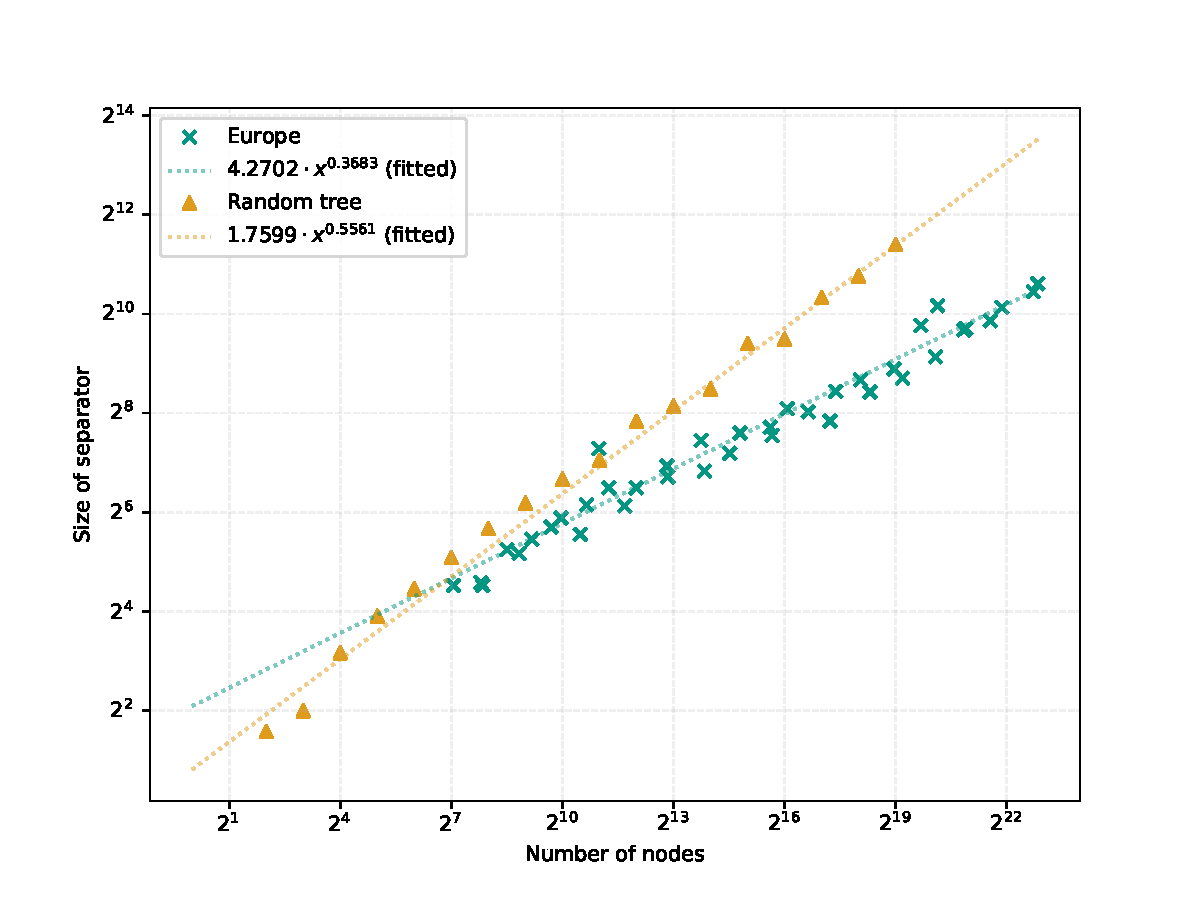
\includegraphics[width=0.6\linewidth]{graphics/diameters.pdf}
	\caption{The plot shows the diameter (y-axis) as a function of the number of nodes \(n\) (x-axis, log scale).}
	\label{fig:diameter_karlsruhe}
\end{figure}

Following the generation of the initial random spanning tree, we proceed to the second step: adding edges randomly between pairs of non-adjacent vertices.
This edge addition continues until the target average degree of \(2.5\) is reached for the entire graph.
The resulting graphs, by construction, lack the inherent locality often present in road networks.
A consequence of adding these random edges is a notable decrease in the graph diameter.
For example, graphs generated with one million nodes using this method exhibit diameters of approximately 40.

These synthetic graphs do not replicate the small separator sizes observed in real-world road networks.
Experiments yielded large top-level separators, whose sizes scaled approximately linearly with the graph size \(n\), i.e., as \bigO{n}.
However, separators found during subsequent recursive partitioning behaved differently: their sizes were significantly smaller than this linear trend would predict for the corresponding subgraph sizes.
We attribute this deviation to structural changes in the subgraphs induced by the partitioning process.
Specifically, the large top-level separators often remove a significant fraction of the non-tree edges that were originally added to achieve the target average degree of approximately \(2.5\) in the parent graph.
Consequently, the resulting subgraphs become sparser, our observations showed a decrease in average degree to approximately \(2.2\), and increasingly dominated by their underlying tree structure.
This shift means these subgraphs effectively belong to a different, more tree-like graph class than initially generated, which naturally leads to smaller relative separator sizes.
The separator scaling is illustrated in \cref{fig:same_degree}.



\begin{figure}[tbhp]
	\centering
	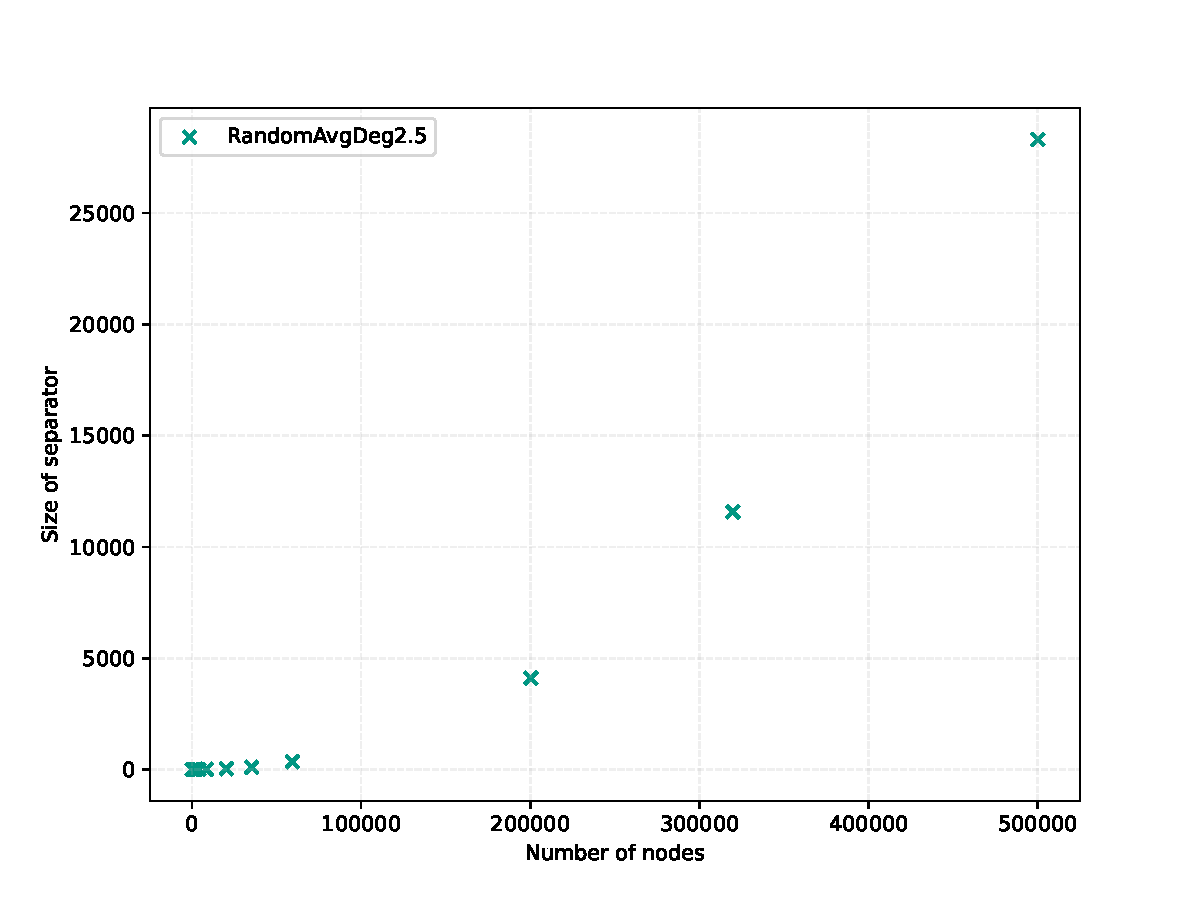
\includegraphics[width=0.6\linewidth]{graphics/RandomAvgDeg2.5.pdf}
	\caption{Separator sizes observed in random graphs generated with an average degree matching the DIMACS Europe road network (\( \approx 2.5 \)). Separators were computed using FlowCutter (tests with KaHIP yielded similar asymptotic scaling).}
	\label{fig:same_degree}
\end{figure}

We also conducted experiments to generate graphs that match not just the average degree but also the specific degree distribution of a reference road network.
This process involved starting with a random tree and then adding edges subject to constraints: an edge \((u, v)\) was incorporated only if doing so would not cause either vertex \(u\) or \(v\) to exceed the degree count specified for them by the target distribution, which was sampled from the road network.
The separator results from this more refined approach were largely similar to those from graphs matching only the average degree.
It is important to note, however, that precisely replicating a target degree distribution with this method is not possible.
While the maximum degree in the generated graphs generally aligns with that of the reference network, discrepancies emerge, particularly for nodes with a higher degree.
The underlying random spanning tree structure tends to produce a higher proportion of such nodes compared to actual road networks.
For instance, in synthetic graphs designed to match the Europe dataset \cite{ptv_group_dimacs-europe_2009}, approximately 1.8\% of vertices had a degree of 5 or greater, exceeding the 0.2\% observed in the real dataset.
Thus, our process achieves an approximation of the target distribution.
Nevertheless, we posit that this approximation is sufficiently close for our investigation, as the relatively small fraction of vertices with degrees deviating from the target constraints is unlikely to fundamentally alter the observed separator scaling behavior for this graph class.
These findings reinforce the suggestion that the specific degree distribution, in isolation, is likely insufficient to fully explain the empirically observed small separators.
Nevertheless, the low average degree remains a noteworthy property.
While a lower average degree may not fundamentally alter the inherent asymptotic separator scaling characteristic of a specific graph class, it often correlates with smaller constant factors in the observed separator sizes,
the practical effect of sparsity on separator magnitudes will be discussed further in a subsequent section.
Beyond the influence of average degree on constant factors, it is also crucial to recognize that neither a low average degree nor a specific sparse degree distribution is a strict prerequisite for achieving small separators.
Indeed, graphs can be constructed that possess both deliberately small separators (as a function of \(n\)) and a high average degree.
Consider, for instance, the following recursive graph generation scheme designed to produce a graph on \(n\) vertices with a target separator of size \(s(n)\) (e.g., \(s(n) = n^{1/3}\)):
First, a separator clique \(S\) on \(s(n)\) vertices, denoted \(K_{s(n)}\), is designated.
Then, two subgraphs, \(G_1\) and \(G_2\), each containing approximately \((n-s(n))/2\) vertices, are generated recursively by the same procedure (with a base case, such as returning a clique \(K_n\), for small \(n\), e.g., when \(n \le 2\)).
Finally, every vertex in \(G_1\) is connected to every vertex in \(S\), and likewise, every vertex in \(G_2\) is connected to every vertex in \(S\).
By construction, the set \(S\) (forming a \(K_{s(n)}\)) is a separator of size \(s(n)\) that partitions the graph into \(G_1\) and \(G_2\).
Despite this small, built-in separator, the average degree of the resulting graph can be substantial.
For example, using \(s(n) = n^{1/3}\), a graph of \(n=10^4\) vertices generated via this method has an average degree of approximately 169 and a maximum degree of 6202.
This example illustrates that specific structural properties enabling small separators can coexist with high overall edge density, suggesting that the global organization of edges, beyond mere sparsity, significantly influences separator characteristics.

\section{Locality}
\label{sec:synthetic:locality}

Our investigation into locality begins by exploring how \enquote{closeness} defined by an existing network structure, rather than by direct geometric proximity in an embedding, influences graph properties.

\paragraph{Tree Locality}

For this first approach, we simulate locality by considering distances within an initial random spanning tree, which serves as a foundational sparse connected graph.
The premise is that vertices closer to each other along paths in this underlying tree are more likely candidates for new, direct connections, potentially reflecting how topological proximity in an existing network might drive the addition of new links.
To implement this, we begin by generating a random spanning tree using Broder's algorithm \cite{broder_generating_1989}.
Subsequently, edges are added between non-adjacent vertices until a target average degree is achieved.
While many experiments in this thesis use a target average degree of approximately \(2.5\) to emulate road networks, a different value is chosen for this specific model.
The choice of average degree primarily influences the constant factors of the separator scaling, rather than the underlying asymptotic growth of the graph class.
In other contexts, an average degree of \(2.5\) effectively approximates the constant factors of road network separators.
For this tree-distance-based locality model, however, an average degree of approximately 3 is required to achieve a comparable alignment of these constant factors.
To incorporate this form of locality, the probability of adding an edge between two vertices \(u\) and \(v\) is made dependent on their distance within this initial spanning tree \(T\), \( \text{dist}_T(u, v) \).
Specifically, we select a random vertex \(x\) and choose a second vertex \(y\) with a probability related to \(f(\text{dist}_T(x, y))\), where \(f\) is a decreasing function.
The computation of tree distances \(\text{dist}_T(x, y)\) for numerous candidate pairs \((x,y)\) is a critical step in this edge addition phase.
For each randomly selected vertex \(x\) and potential neighbor \(y\), a Breadth-First Search (BFS) is performed within the tree \(T\) to find \(\text{dist}_T(x, y)\).
While BFS on a tree is linear in the number of vertices \(n\), repeated invocations for many pairs prove computationally intensive for larger graphs.
However, the approach is highly parallelizable since each BFS is an independent computation on the fixed tree structure.
Capping the BFS search for \(y\) (e.g., after a fixed number of hops or visited nodes, such as 50,000), while significantly reducing computational overhead did not achieve the desired locality effect.
We observe an artificial steep cutoff in the observed separator characteristics once graph or component sizes effectively exceed the scale imposed by this search limit.
Experiments exploring various decay functions \(f\) yield diverse results.
Simple functions like \( f(\text{dist}) = 1/\text{dist} \) result in graphs that still exhibit large top-level separators scaling as \bigO{n}, although subgraphs from nested dissection show the previously noted superlinear decrease in separator size.
Conversely, rapidly decaying functions like \( f(\text{dist}) = 2^{-\text{dist}} \) produce graphs with separators of almost constant size, likely because the graph structure remains very close to that of the initial tree, with insufficient long-range connections.
Through further experimentation and fine-tuning, it is found that a function of the form \( f(\text{dist}) = 1/\text{dist}^{3.3} \) is able to produce separator sizes that closely approximate the desired \bigO{n^{0.37}} scaling (see \cref{fig:tree_dist_best_fit_scaling}).
\cref{fig:tree_dist_locality_scaling} provides a visual comparison of the separator sizes for various decay functions.

\begin{figure}[tbhp]
	\centering
	\begin{subfigure}{0.45\linewidth}
		\centering
		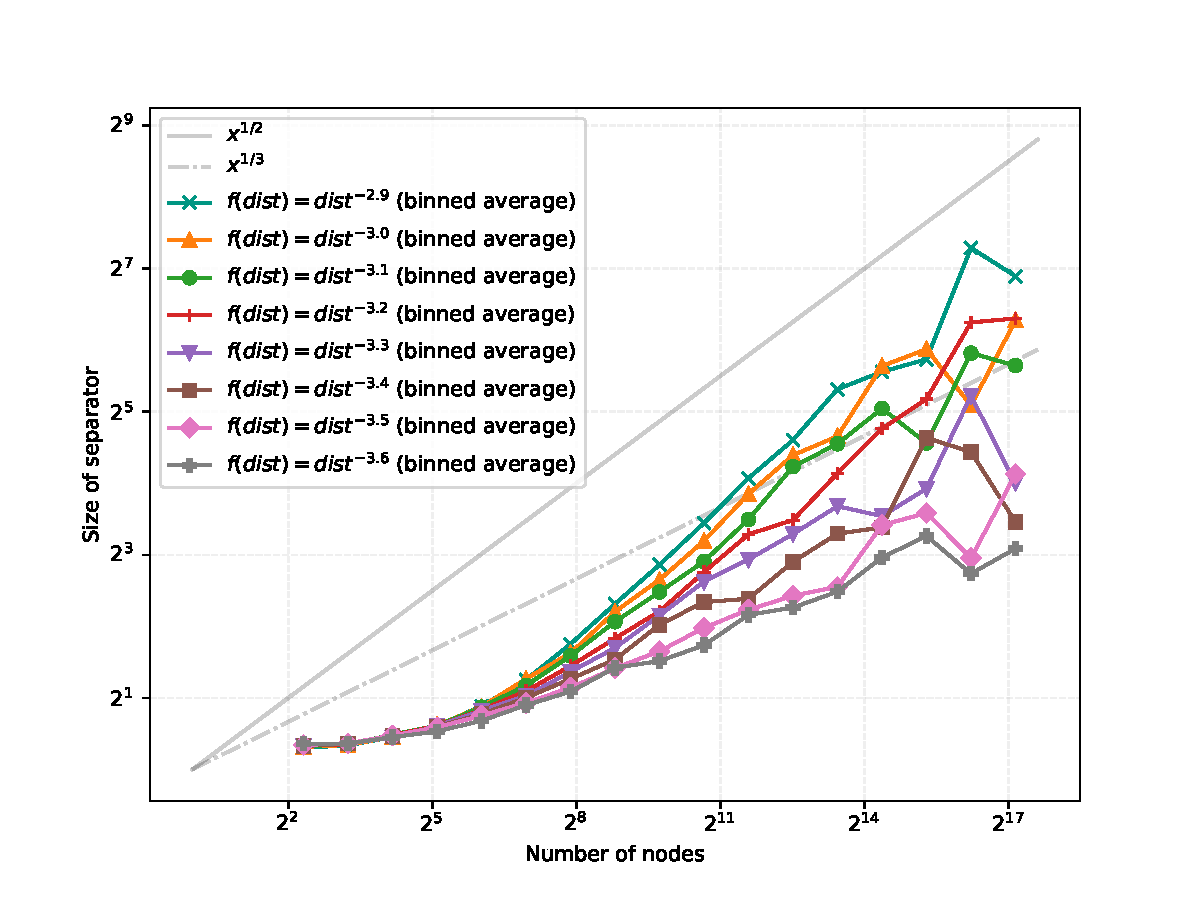
\includegraphics[width=\linewidth]{graphics/tree_local_pow_overview.pdf}
		\caption{Separator scaling for various decay functions \(f\).}
		\label{fig:tree_dist_compare_functions}
	\end{subfigure}
	\hfill
	\begin{subfigure}{0.45\linewidth}
		\centering
		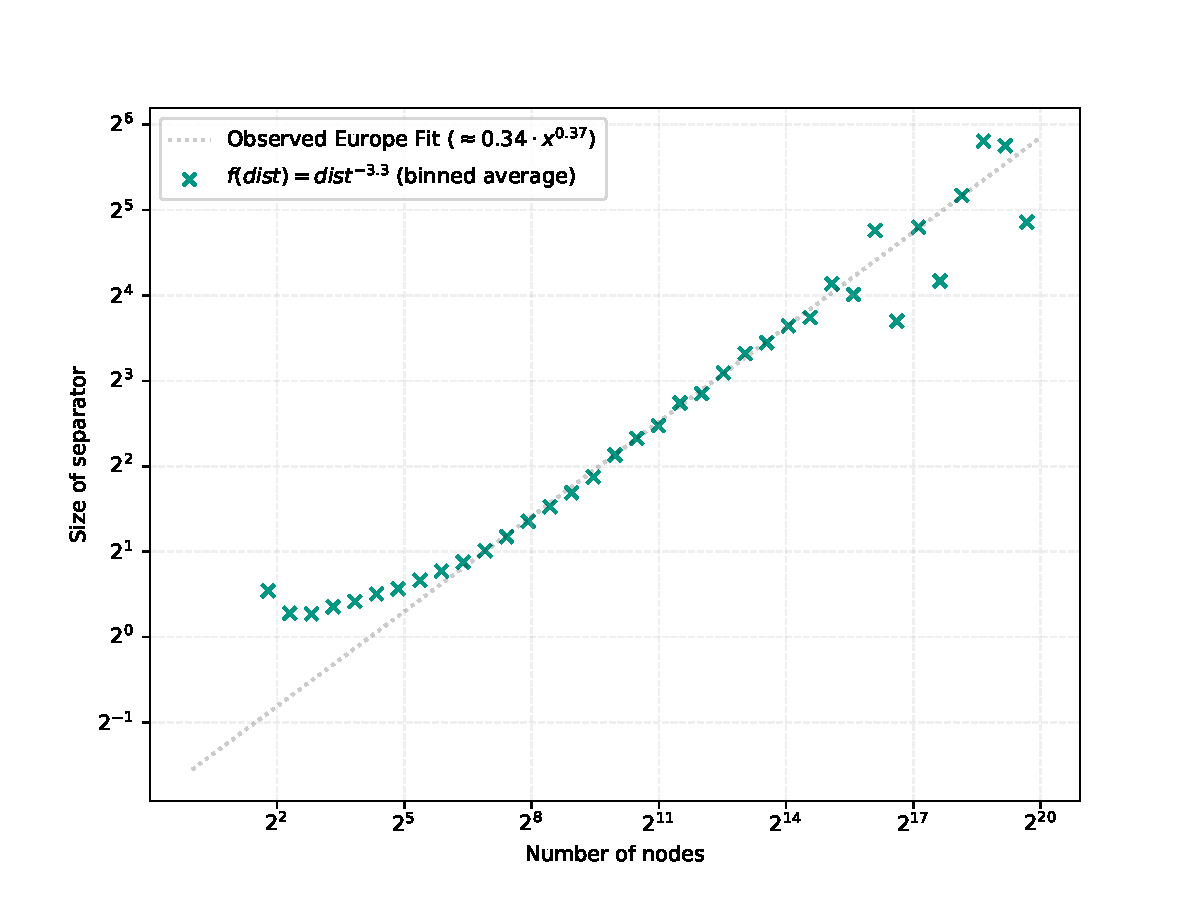
\includegraphics[width=\linewidth]{graphics/tree_locality_33_1000000.pdf}
		\caption{Separator scaling for \(f(\text{dist}) = 1/\text{dist}^{3.3}\) with line fit.}
		\label{fig:tree_dist_best_fit_scaling}
	\end{subfigure}
	\caption{Separator size scaling for graphs generated with tree-distance-based locality, comparing various decay functions and highlighting the fit for \(f(\text{dist}) = 1/\text{dist}^{3.3}\). Separators were computed using FlowCutter (tests with KaHIP yielded similar asymptotic scaling).}
	\label{fig:tree_dist_locality_scaling}
\end{figure}

Despite achieving the target scaling with \(f(\text{dist}) = 1/\text{dist}^{3.3}\), this result offers limited insight into the intrinsic structural properties of real road networks that lead to their small separators.
The success with this specific, empirically derived exponent appears to be more a consequence of parameter tuning within this particular generative model (a random tree backbone augmented by edges based on tree distance) rather than an elucidation of fundamental graph characteristics.
While the general concept of incorporating locality based on distances within an existing network structure remains potentially insightful, as such a metric might capture aspects beyond mere Euclidean distance, like travel time reduction incentives, our preliminary results with simpler functions indicate a high sensitivity to the choice of \(f\).
Achieving the target \bigO{n^{0.37}} scaling with an empirically derived function like \(f(\text{dist}) = 1/\text{dist}^{3.3}\) appears to be an outcome of model-specific parameter tuning rather than a revelation of intrinsic road network properties responsible for their small separators.
Given these considerations and the decision to prioritize other structural properties like geometric locality, planarity, and explicit hierarchy, we opt not to pursue an exhaustive search for an optimal or more interpretable tree-distance decay function within the scope of this work.

\paragraph{Geometric Locality}

Our second approach incorporates geometric locality directly.
The core idea is to construct a graph starting with a basic connected structure and then augment it by adding only edges that connect geometrically close vertices, until a target average degree (e.g., \(2.5\)) is achieved.
To establish a meaningful threshold for 'closeness', we relate it to the natural scale derived from the spatial distribution of points.
Specifically, we first sample \(n\) points uniformly within a defined spatial domain (e.g., a circle).
We then compute the Minimum Spanning Tree (MST) of these points using Euclidean distances, via Kruskal's algorithm \cite{kruskal_shortest_1956}.
The maximum edge length found within this MST, denoted \(\ell_{\max}\), serves as our threshold distance, capturing a characteristic length scale of the initial sparse connection of the points.
The graph generation then proceeds by initially taking the edges of the MST.
Subsequently, additional edges \((u, v)\) between non-adjacent vertices are iteratively added, but crucially, only if their Euclidean distance is less than or equal to the threshold \(\ell_{\max}\).
This edge addition process continues until the overall graph reaches the target average degree of \(2.5\).
For efficient implementation of the edge addition step, we utilize spatial queries: for a randomly selected vertex \(u\), we query for potential neighbors \(v\) within the radius \(\ell_{\max}\) and randomly select one to connect to, avoiding multi-edges and self-loops.
Despite incorporating this explicit geometric constraint, the resulting synthetic graphs fail to exhibit the desired small separator sizes characteristic of road networks.
To analyze the separator properties of these graphs, we computed recursive separators.
Our experiments using these methods indicate that separators in these geometrically generated graphs scale approximately as \bigO{n^{1/2}}.
This outcome is visualized in \cref{fig:geometric_locality_separators}.

\begin{figure}[tbhp]
	\begin{subfigure}{0.35\linewidth}
		\centering
		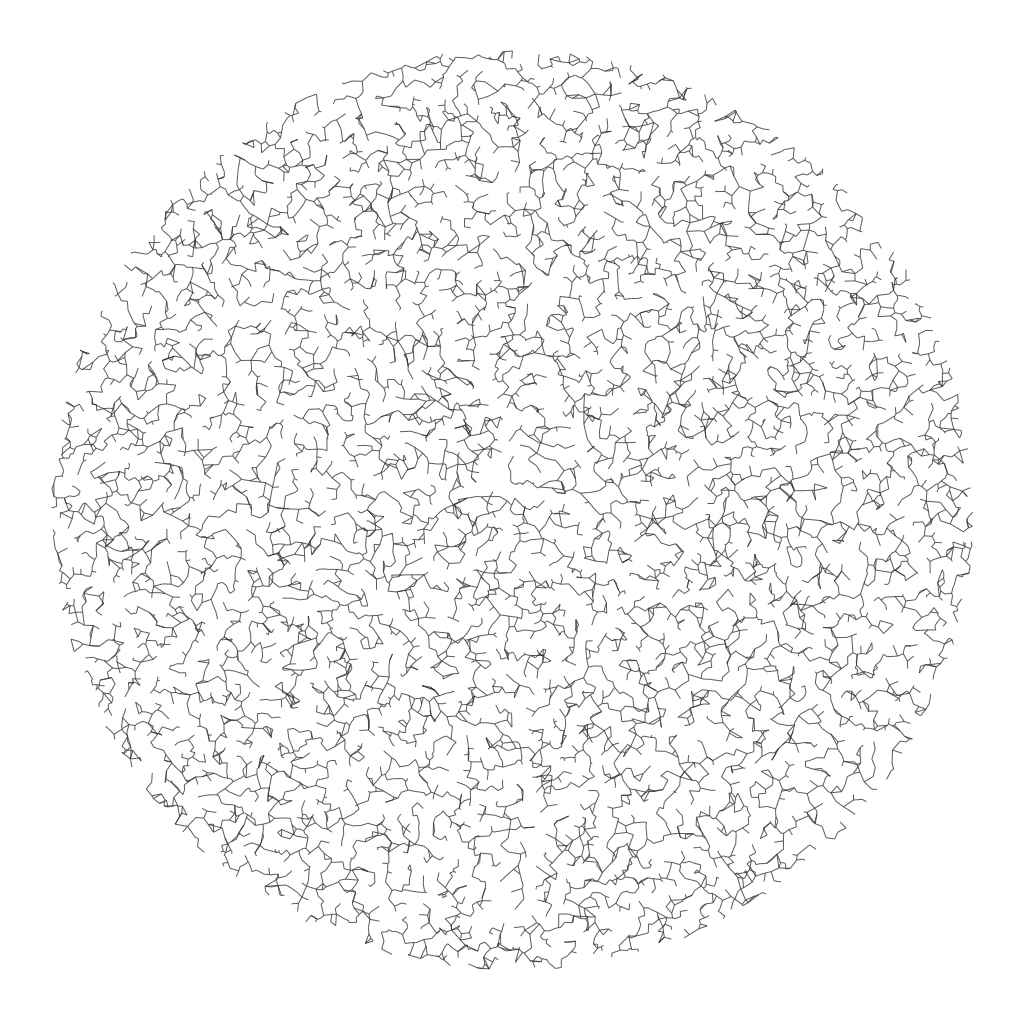
\includegraphics[width=\linewidth]{graphics/local_embedding.png}
		\caption{Visualization of a graph with \(10^4\) nodes generated using the geometric locality method.}
		\label{fig:geometric_locality_graph_viz}
	\end{subfigure}
	\hfill
	\begin{subfigure}{0.55\linewidth}
		\centering
		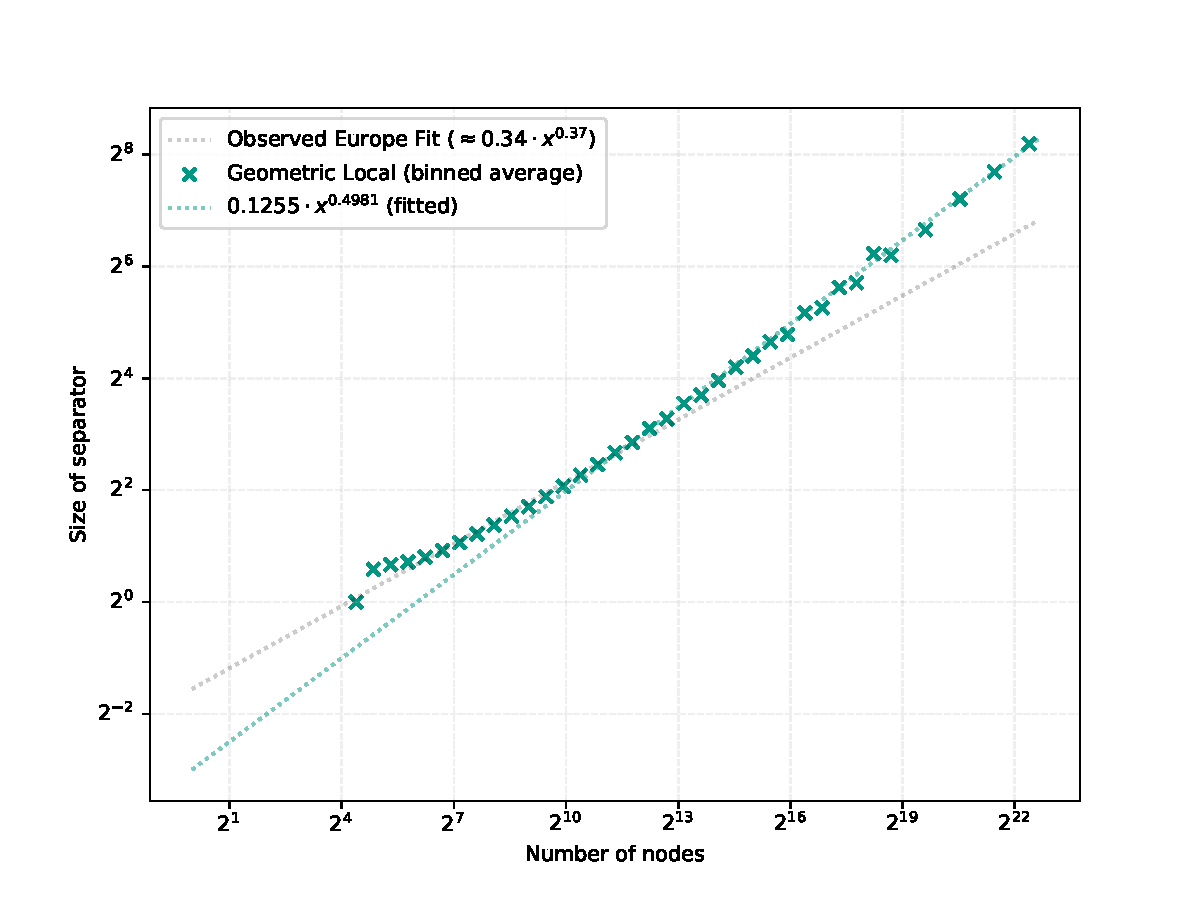
\includegraphics[width=\linewidth]{graphics/sep_local_embedding.pdf}
		\caption{Separator size scaling for synthetic graphs generated with geometric locality. The fit shown excludes subgraphs with \( \le 1000 \) vertices due to their disproportionately large separators. }
		\label{fig:geometric_locality_sep_plot}
	\end{subfigure}
	\caption{Synthetic graph generation using geometric locality and analysis of separator sizes. Separators were computed using InertialFlowCutter (tests with FlowCutter and KaHIP yielded similar asymptotic scaling).}
	\label{fig:geometric_locality_separators}
\end{figure}

An alternative strategy we investigate for incorporating geometric locality is the construction of k-Nearest Neighbor (k-NN) graphs.
In this model, each vertex connects via an edge to its \(k\) geographically closest neighbors, with proximity defined by the Euclidean distance between their embedded point coordinates.
This approach does not utilize an underlying tree structure like some previously discussed methods.
Connectivity in a k-NN graph is not guaranteed, however, the size of the largest connected component generally increases with the value of \(k\).
For instance, with uniformly sampled points, a \(k\) as small as 3 often yields a primary connected component encompassing approximately 98\% of all vertices.
The average degree of the resulting graph is directly influenced by \(k\).
For point sets with non-uniform distributions, a larger \(k\) is typically required to achieve a similar level of overall connectivity.
Our objective is to identify the smallest \(k\) that results in a largely connected graph, while also aiming for a low average degree, comparable to those of sparse road networks.
The construction of k-NN graphs can be performed efficiently: following an initial \bigO{n \log n} precomputation to build a spatial index such as a k-d tree, identifying the \(k\) nearest neighbors for each of the \(n\) vertices takes approximately \bigO{k \log n} time per vertex, resulting in a total construction time of roughly \bigO{nk \log n}.
Our experiments show that k-NN graphs generated in this manner also exhibit separator sizes that scale approximately as \bigO{n^{1/2}} as seen in \cref{fig:knn_graph_analysis}.
\begin{figure}[tbhp]
	\centering
	\begin{subfigure}{0.35\linewidth}
		\centering
		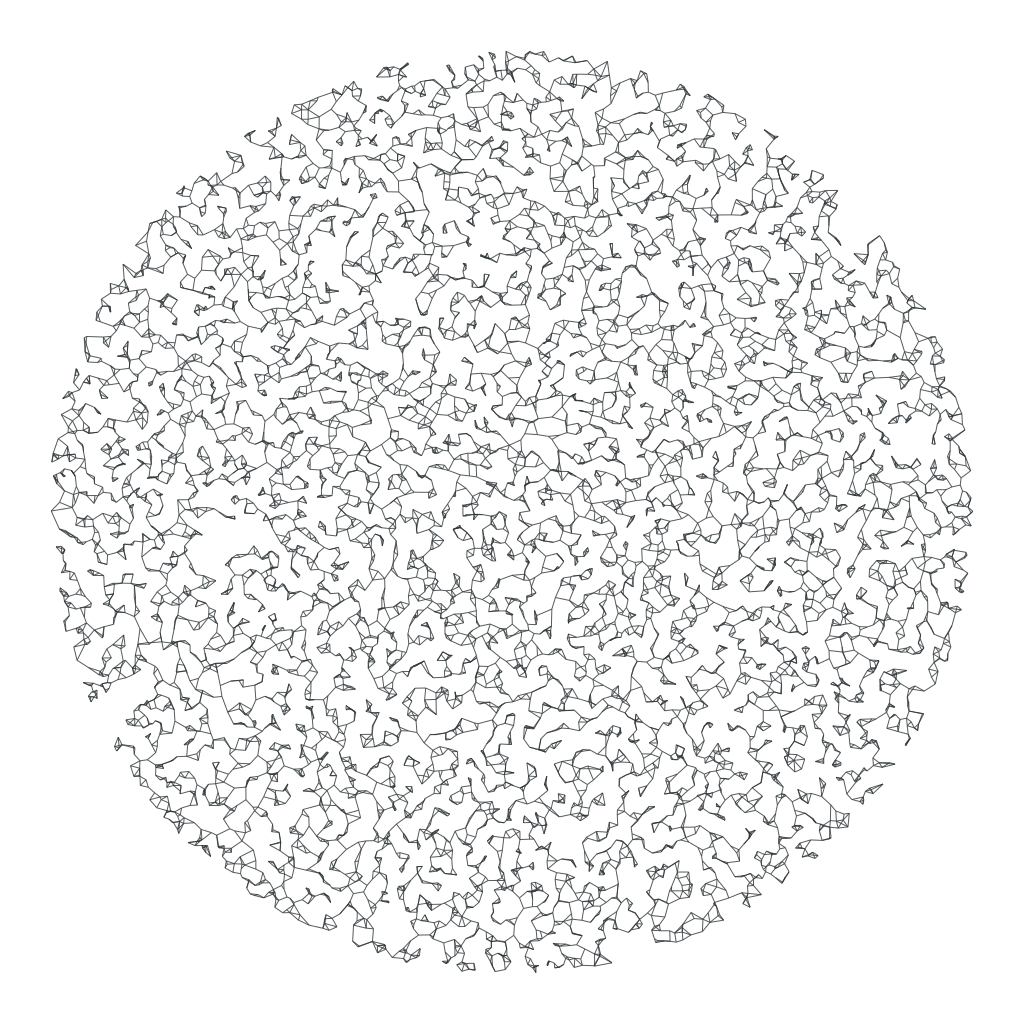
\includegraphics[width=\linewidth]{graphics/knn.png}
		\caption{Visualization of a k-NN graph (for \(k=3\)) generated from \(n \approx 10^4\) uniformly sampled points.}
		\label{fig:knn_graph_structure_viz}
	\end{subfigure}
	\hfill
	\begin{subfigure}{0.55\linewidth}
		\centering
		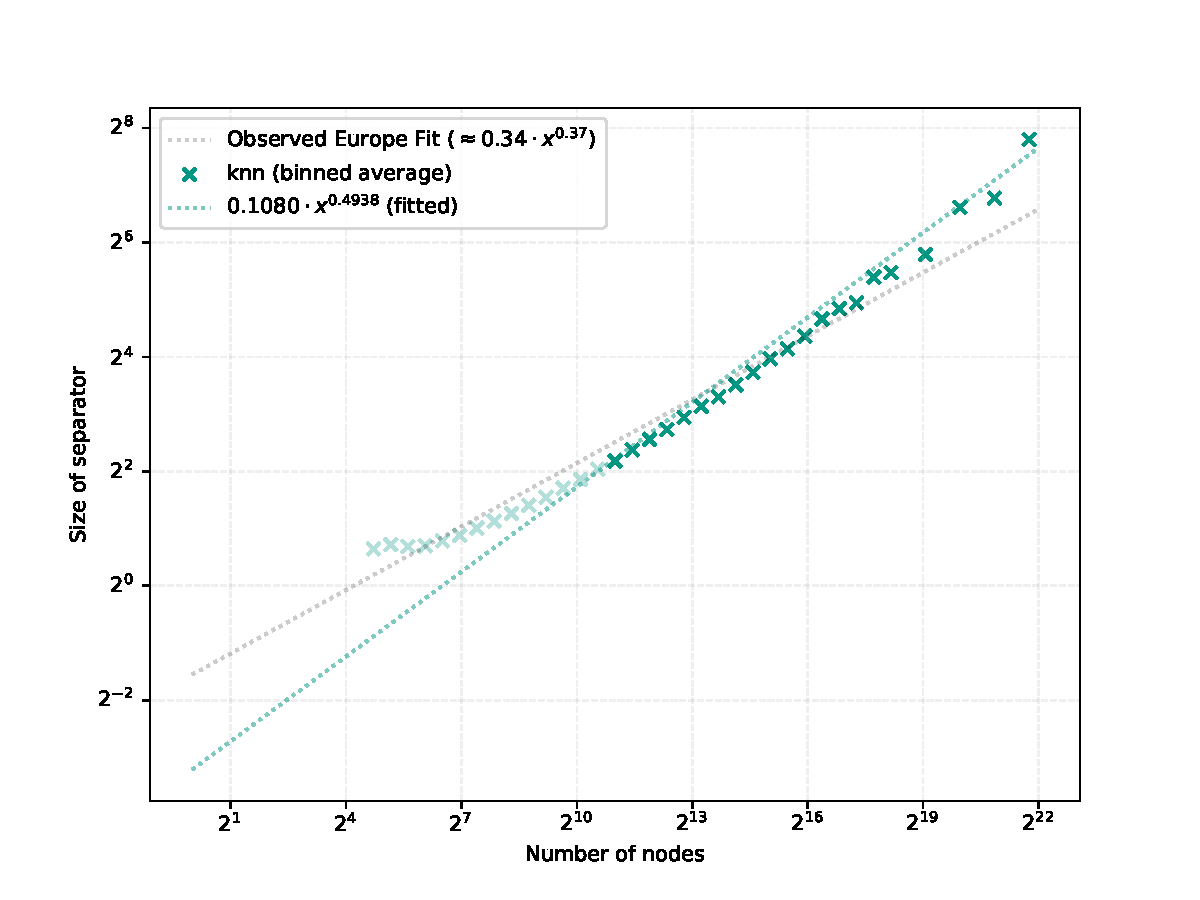
\includegraphics[width=\linewidth]{graphics/knn_seps.pdf}
		\caption{Separator size scaling for k-NN graphs \(k=3\), showing approximately \bigO{n^{1/2}} behavior.}
		\label{fig:knn_graph_sep_scaling_plot}
	\end{subfigure}
	\caption{Analysis of k-Nearest Neighbor (k-NN) graph of uniformly sampled points and separator scaling. Separators were computed using InertialFlowCutter (tests with FlowCutter and KaHIP yielded similar asymptotic scaling).}
	\label{fig:knn_graph_analysis}
\end{figure}

The results from the geometric locality approach suggest that merely combining low average degree with this specific form of locality is insufficient to reproduce the cubic root separator sizes of road networks.

\paragraph{Real-World Implications}

It is worth considering the practical implications of different asymptotic growth rates for separator sizes within the typical scale of road networks.
While \bigO{c_1\cdot n^{1/3}} and \bigO{c_2 \cdot n^{1/2}}, with \(c_2 \ll c_1\), diverge for large \(n\), the actual separator sizes for graphs up to around 20 million vertices are similar.
The performance of algorithms leveraging graph separators in real-world applications may be more influenced by the absolute sizes of separators achievable in practice, compared to a specific scaling model.
Performance gains, for example for CCH \cite{dibbelt_customizable_2016}, could potentially be realized even if the separators behave like \(c \cdot n^{1/2}\) for a sufficiently small \(c\), as the absolute separator sizes remain manageable for networks of practical relevance.

\paragraph{Initial Deviations in Separator Scaling}

Our synthetic graphs generated using the geometric locality approach exhibit a notable initial deviation in their separator scaling at small graph sizes.
As visualized in the histogram in \cref{fig:local_embedding_hist_deviation}, there is an initial peak in relative separator size for small subgraphs, which then decreases before the data align with the more dominant scaling trend observed for larger graphs.
This behavior is similar to the initial scaling deviations present in real road networks.
This correspondence is noteworthy, as it suggests that our geometric locality model, despite failing to replicate the overall asymptotic separator scaling, may capture certain structural properties that are relevant at smaller graph scales and also present in actual road networks.

\begin{figure}[tbhp]
	\centering
	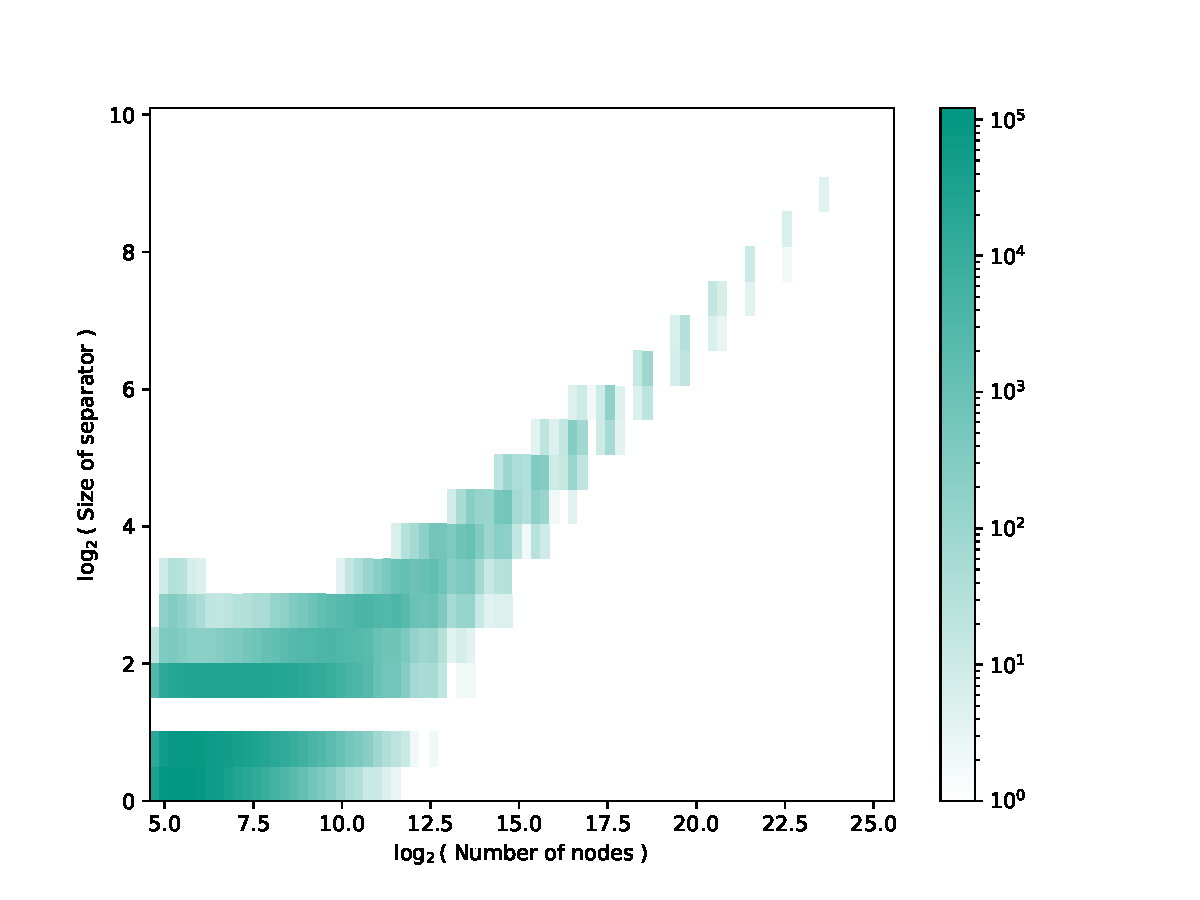
\includegraphics[width=0.6\linewidth]{graphics/local_embedding-hist.pdf}
	\caption{Histogram of separator sizes for synthetic graphs using geometric locality, illustrating an initial peak in relative separator size for small subgraphs (around \(2^6\) nodes). Separators were computed using InertialFlowCutter (tests with FlowCutter and KaHIP yielded similar asymptotic scaling).}
	\label{fig:local_embedding_hist_deviation}
\end{figure}




\paragraph{Minimum Spanning Trees from Higher-Dimensional Embeddings}
\label{sec:synthetic:mst}

Observing that real road networks often exhibit diameters smaller than the \bigO{n^{1/2}} found in our random tree models, we sought to determine if an initial tree structure with an intrinsically smaller diameter could lead to graphs with correspondingly smaller separators after edge augmentation.
This motivated an exploration of generating initial trees as Minimum Spanning Trees (MSTs) of points sampled in \(d\)-dimensional Euclidean space, since the diameter of such an MST on \(n\) random points in \(d\)-space (for \(d \ge 2\)) is typically \bigO{n^{1/d}}.
Our experiments focused on the case where \(d=3\), for which the MST diameter is approximately \bigO{n^{1/3}}.
This involved sampling \(n\) points uniformly in 3D space and computing their MST.
When edges were subsequently added to such 3D-MSTs to achieve a target average degree, the resulting graphs exhibited separators that scaled as \bigO{n^{2/3}}.
This scaling aligns with a general geometric intuition: a \(d\)-dimensional hypervolume containing \(n\) points is naturally bisected by a \((d-1)\)-dimensional separator.
If the characteristic linear extent of the volume is proportional to \(n^{1/d}\), the \((d-1)\)-dimensional measure (e.g., area for \(d=3\), length for \(d=2\)) of such a separator would be proportional to \((n^{1/d})^{d-1} = n^{(d-1)/d}\).
For \(d=2\), this yields the familiar \bigO{n^{1/2}} scaling for planar-like separators, and for our \(d=3\) experiment, it corresponds to the observed \bigO{n^{2/3}}.
While this suggests a general hypothesis that augmenting MSTs from \(d\)-dimensional point sets might lead to graphs with \bigO{n^{(d-1)/d}} separators, this avenue was not pursued further.
Since for \(d=3\) the \bigO{n^{2/3}} separators do not offer an improvement over the \bigO{n^{1/2}} separators of planar graphs in the context of finding exceptionally small separators (and higher dimensions \(d > 3\) would yield even larger exponents as \((d-1)/d \to 1\)), this specific line of inquiry was not extended.

\section{Planarity}
\label{sec:synthetic:planarity}

We examine separator properties in two classes of planar graphs: grids and Delaunay triangulations.
These serve as fundamental theoretical models for planar structures relevant to the study of road networks due to their near-planarity.
In our study, these graph classes are sparsified to achieve a low average degree (approximately \(2.5\)), reflecting the sparsity observed in road networks.
It is important to note that both of these models inherently introduce strong geometric locality, a property not required by all planar graphs.
Our focus on these specific classes therefore introduces a bias towards investigating planar graphs that also possess this structural characteristic.

\subsection{Grids}
\label{sec:synthetic:grid}

Our initial investigation focuses on grid graphs, a fundamental class known to possess separators scaling as \bigO{n^{1/2}}.
To align their sparsity with road networks, we generate modified grids with an average degree of approximately \(2.5\).
The generation process starts with a square two-dimensional grid graph.
Edges are then removed uniformly at random until the target average degree is reached over the entire graph.
Subsequently, we identify and utilize the largest connected component for analysis.
We observe that even without explicit mechanisms to prevent disconnection during edge removal, the largest connected component typically encompasses a large fraction of the initial vertices.
Analysis of these sparse grid graphs reveals separator sizes consistent with the \bigO{n^{1/2}} asymptotic behavior of complete grids.
However, the constant factor associated with this scaling appears to be relatively small.
Consequently, although the asymptotic limit behavior differs from the \bigO{n^{1/3}} scaling empirically observed for road networks, the absolute separator sizes in these sparse grids are numerically similar to those of road networks for graphs up to typical sizes (e.g., around 20 million nodes).
This finding highlights that sparsity, even within a simple planar structure like a grid, can lead to separators that are small in absolute terms for practical graph dimensions.
\Cref{fig:sparse_grid_separators} illustrates a sample sparse grid and the observed separator scaling.

\begin{figure}[tbhp]
	\centering
	\begin{subfigure}{0.35\linewidth}
		\centering
		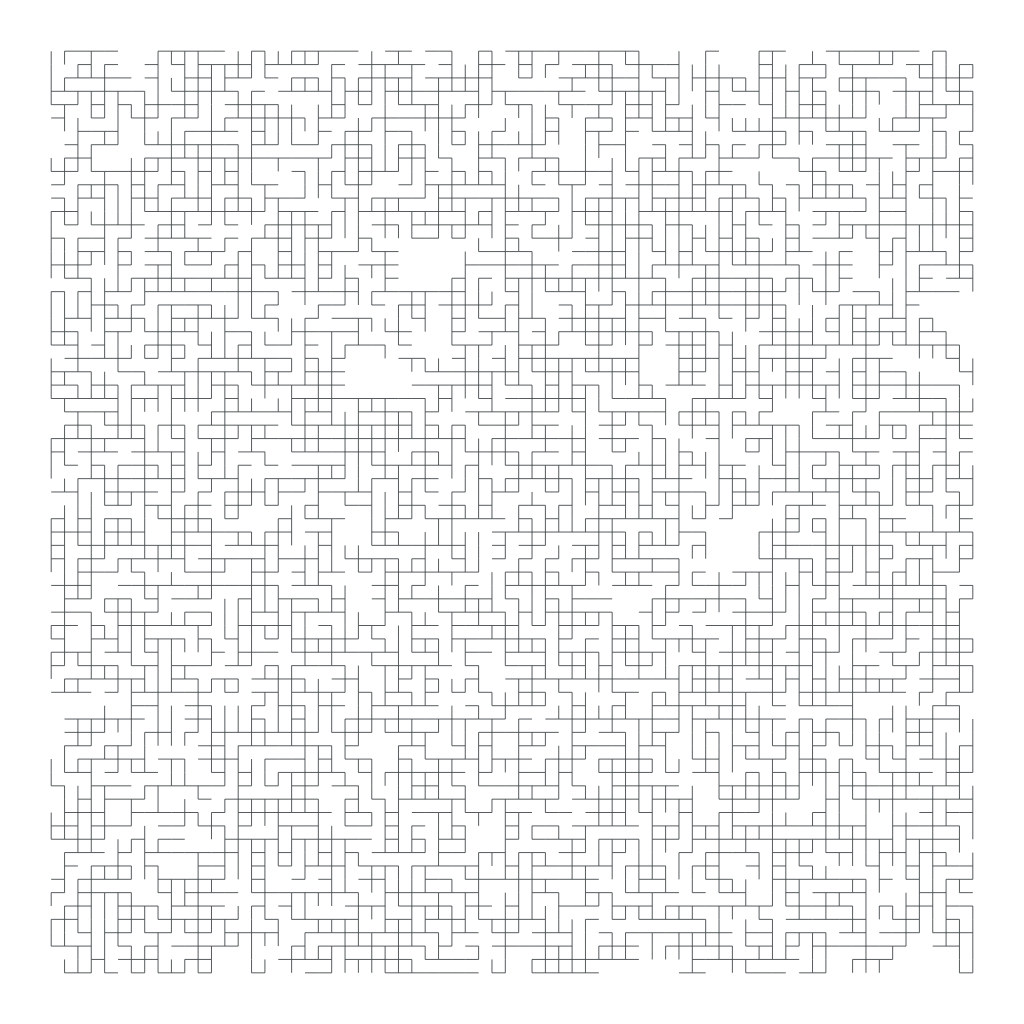
\includegraphics[width=\linewidth]{graphics/grid_avg_deg.png}
		\caption{Visualization of the largest connected component of a grid graph with \(\approx 10\text{K}\) nodes after random edge removal to achieve an average degree of \(2.5\).}
		\label{fig:sparse_grid_viz}
	\end{subfigure}
	\hfill
	\begin{subfigure}{0.55\linewidth}
		\centering
		\includegraphics[width=\linewidth]{graphics/sep_grid_avg_deg.png}
		\caption{Separator size scaling for sparse grid graphs (average degree \(2.5\)). Separator sizes scale approximately as \bigO{n^{1/2}}, but with a small constant factor leading to absolute sizes comparable to road networks at practical scales. The fit shown excludes subgraphs with \( \le 1000 \) vertices due to their disproportionately large separators.}
		\label{fig:sparse_grid_sep_plot}
	\end{subfigure}
	\caption{Analysis of sparse grid graphs with average degree \(2.5\). Separators were computed using InertialFlowCutter (tests with FlowCutter and KaHIP yielded similar asymptotic scaling).}
	\label{fig:sparse_grid_separators}
\end{figure}


Analogous to the earlier example where dense graphs were constructed with a specific separator function, it is also possible to engineer grid-like graphs to exhibit a target separator scaling, such as \(\bigO{n^{1/3}}\).
This approach involves a recursive construction: two smaller grid-like subgraphs, \(G_1\) and \(G_2\), each comprising approximately \(n/2\) vertices, are generated recursively.
These subgraphs are then interconnected.
Instead of forming dense connections or connecting all border vertices, a controlled number of edges, specifically chosen to match the desired separator size (e.g., approximately \(n^{1/3}\) for the combined graph of size \(n\)), are added between \(G_1\) and \(G_2\).
For instance, this can be achieved by selecting approximately \(n^{1/3}\) nodes along the boundary of one subgraph and connecting each to its closest corresponding node on the boundary of the other.
The set of these interconnecting edges (or one of their incident vertices) is, by construction, a separator of the desired \(\bigO{n^{1/3}}\) size.
An example of such a graph and its resulting separator scaling is illustrated in \cref{fig:engineered_grid_sep}.
While this method demonstrates that specific separator sizes can be achieved by deliberate construction in grid-like structures, it offers limited insight into which intrinsic graph properties of real road networks lead to their empirically observed small separators.
The desired scaling is explicitly engineered into the generation process here, rather than emerging naturally from more fundamental characteristics.

\begin{figure}[tbhp]
	\centering
	\begin{subfigure}{0.35\linewidth}
		\centering
		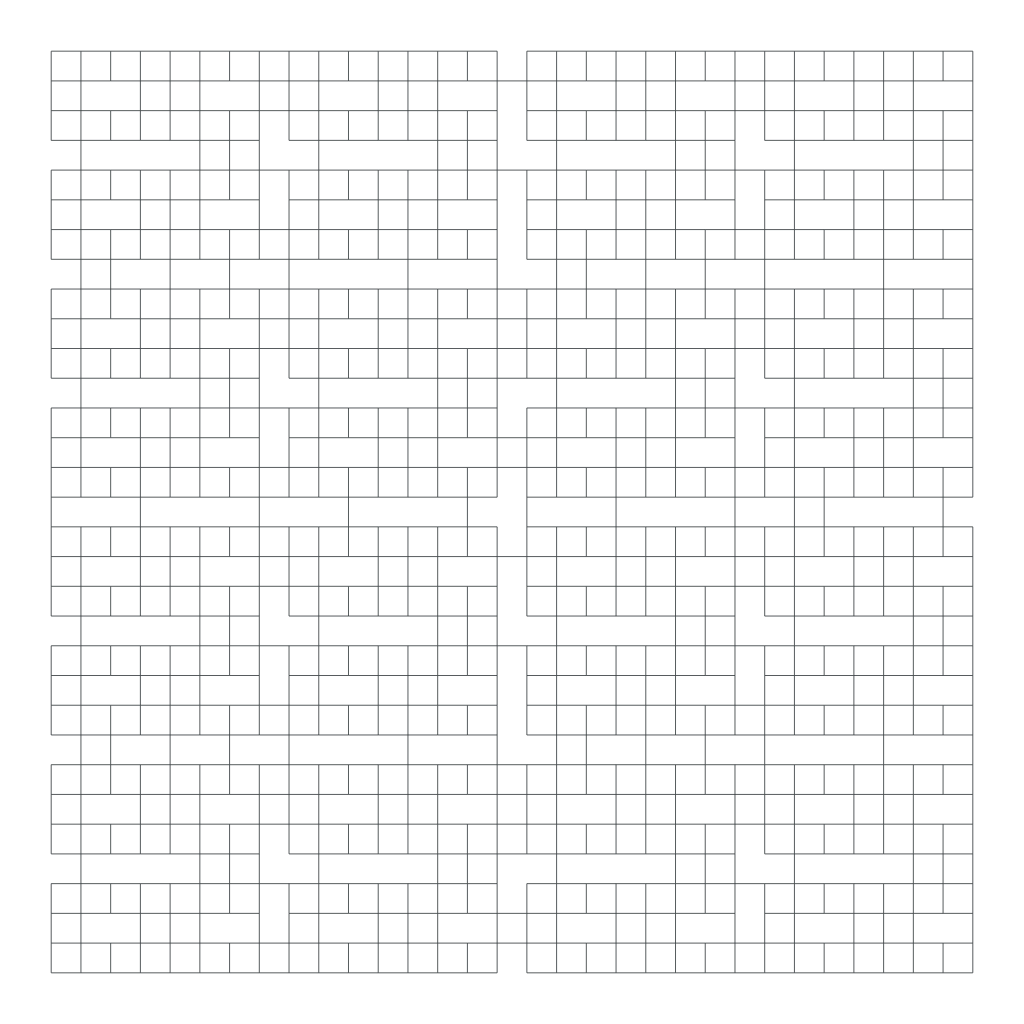
\includegraphics[width=\linewidth]{graphics/cbrt_grid.png}
		\caption{A recursively constructed grid with engineered \(\bigO{n^{1/3}}\) interconnections.}
		\label{fig:engineered_grid_structure_viz}
	\end{subfigure}
	\hfill
	\begin{subfigure}{0.55\linewidth}
		\centering
		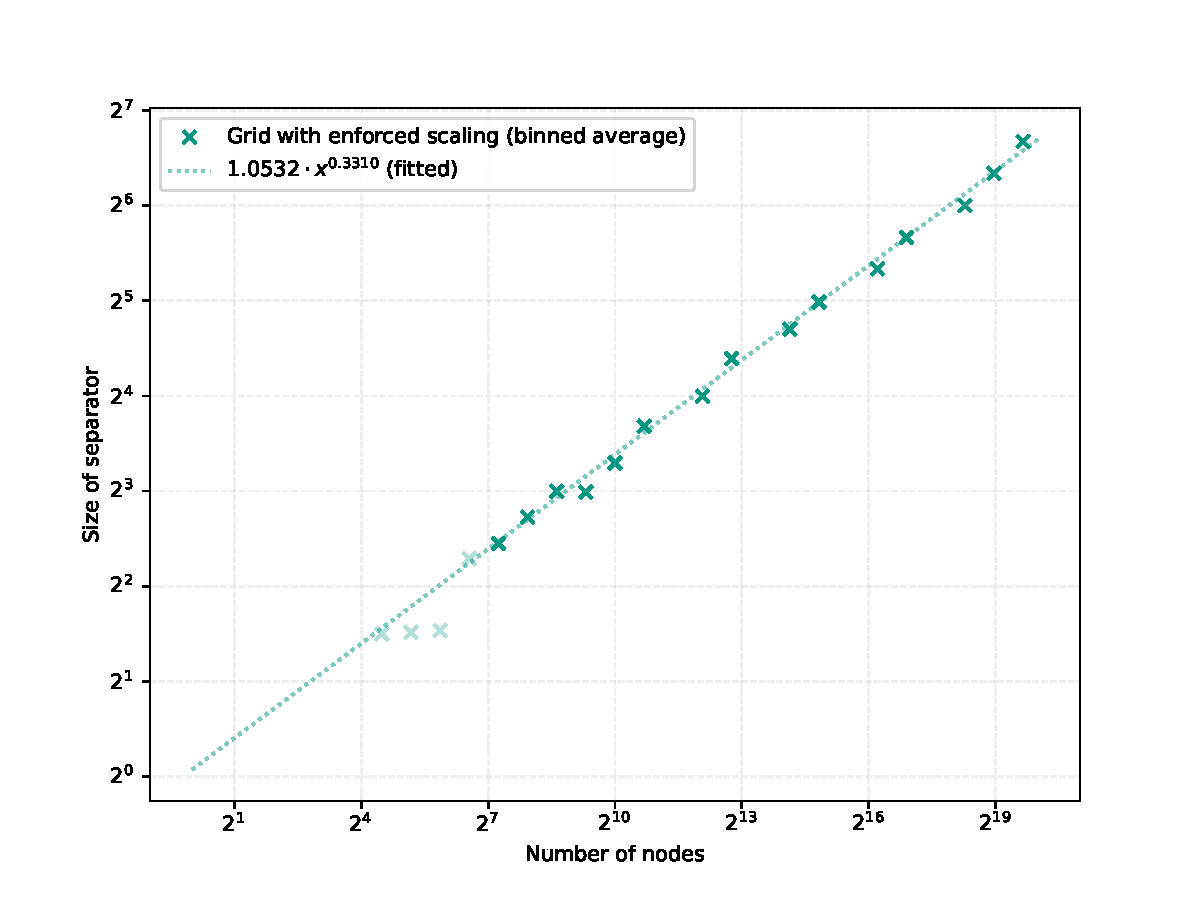
\includegraphics[width=\linewidth]{graphics/cbrt_grid_sep_scaling.pdf}
		\caption{Separator scaling for the engineered grid graph, exhibiting the constructed \(\bigO{n^{1/3}}\) behavior.}
		\label{fig:engineered_grid_sep_plot}
	\end{subfigure}
	\caption{Grid-like graph with engineered separators designed to scale as \(\bigO{n^{1/3}}\). Separators were computed using InertialFlowCutter (tests with FlowCutter and KaHIP yielded similar asymptotic scaling).}
	\label{fig:engineered_grid_sep}
\end{figure}
















\subsection{Delaunay Triangulations and Their Sparse Subgraphs}
\label{sec:synthetic:delaunay_variants}

As a generalization of grid-like structures derived from point sets, Delaunay Triangulations (DT) are fundamental in computational geometry and serve as a basis for generating planar graphs.
A DT for a given set \(P\) of discrete points in a plane is a specific triangulation such that for any triangle in \(DT(P)\), its circumcircle (the unique circle passing through its three vertices) contains no other points from \(P\) in its interior.
This \enquote{empty circumcircle} property ensures that DTs tend to maximize the minimum angle of all triangles in the triangulation, thereby avoiding overly elongated triangles.
Our process for generating a baseline Delaunay graph involves sampling \(n\) points uniformly at random in a two-dimensional space and then computing their full Delaunay triangulation.
Such a DT typically has an average vertex degree around 6. This observation is consistent with Euler's formula for planar graphs (\(|V| - |E| + |F| = 2\)),
for large triangulations, where most faces are triangles and each internal edge is shared by two faces (\(3|F| \approx 2|E|\)), the average degree \(2|E|/|V|\) approaches 6.

Since an average degree of 6 is considerably denser than that of typical road networks (which is closer to \(2.5\)), sparsification is necessary to create more comparable synthetic graphs.
We explore several methods for this:

\paragraph{Random Edge Deletion}

One straightforward sparsification technique, similar to that applied in our grid experiments, involves randomly deleting edges from the full Delaunay triangulation until the target average degree of approximately \(2.5\) is achieved.
The largest connected component of the resulting graph is then used for analysis.

\paragraph{Systematically Defined Subgraphs}

Alternatively, sparser graphs can be derived from the DT by retaining only those edges that satisfy stricter geometric conditions.
Prominent examples of such Delaunay subgraphs include Gabriel Graphs (GG) \cite{gabriel_new_1969} and Relative Neighborhood Graphs (RNG) \cite{toussaint_relative_1980}.
An edge \((u,v)\) is part of a GG if the closed disk whose diameter is the segment \(uv\) contains no other point from the original set \(P\).
An edge \((u,v)\) belongs to an RNG if no third point \(w \in P\) is simultaneously closer to both \(u\) and \(v\) than \(u\) and \(v\) are to each other,
that is, the lune formed by the intersection of two circles of radius \(\text{dist}(u,v)\) centered at \(u\) and \(v\) must be empty of other points.
These definitions lead to the known hierarchical relationship: RNG \(\subseteq\) GG \(\subseteq\) DT.
The RNG is particularly interesting from a network modeling perspective, as its construction criterion can be loosely interpreted in terms of economic viability for infrastructure: a direct road between two points \(u\) and \(v\) might not be constructed if an alternative path via a nearby third point \(w\) (e.g., \(u \to w \to v\)) exists without a significant detour.
For uniformly sampled random points, the RNG yields an average degree of approximately \(2.6\) \cite{buhl_topological_2006}, which is close to the average degree of road networks.

\paragraph{Separator Analysis of Delaunay Variants}

We analyzed the separator properties of these different Delaunay-derived graphs: the full DT, the randomly sparsified DT (target average degree \(2.5\)), the Gabriel Graph, and the Relative Neighborhood Graph, all generated from identical initial point sets to ensure comparability.
Visualizations of these graph structures and their comparative separator scaling are presented in \cref{fig:delaunay_variants_comparison}.
Despite the variations in density, ranging from an average degree of approximately 6 for the full DT down to about \(2.6\) for the RNG, our experiments indicate that the asymptotic separator scaling for all these Delaunay-derived planar graphs remains consistent with \bigO{n^{1/2}}.
The method of sparsification, whether through random edge deletion or by applying systematic geometric rules like those for GG or RNG, primarily influences the constant factors associated with the separator size.
It does not, however, fundamentally alter the \bigO{n^{1/2}} scaling behavior tied to their underlying planar geometric nature.
Even when the average degree very closely matches that of road networks (as in the RNG case), the separator scaling does not approach the \(\approx \bigO{n^{0.37}}\) observed empirically for road networks.

\begin{figure}[tbhp]
	\centering
	\begin{subfigure}{0.3\linewidth}
		\centering
		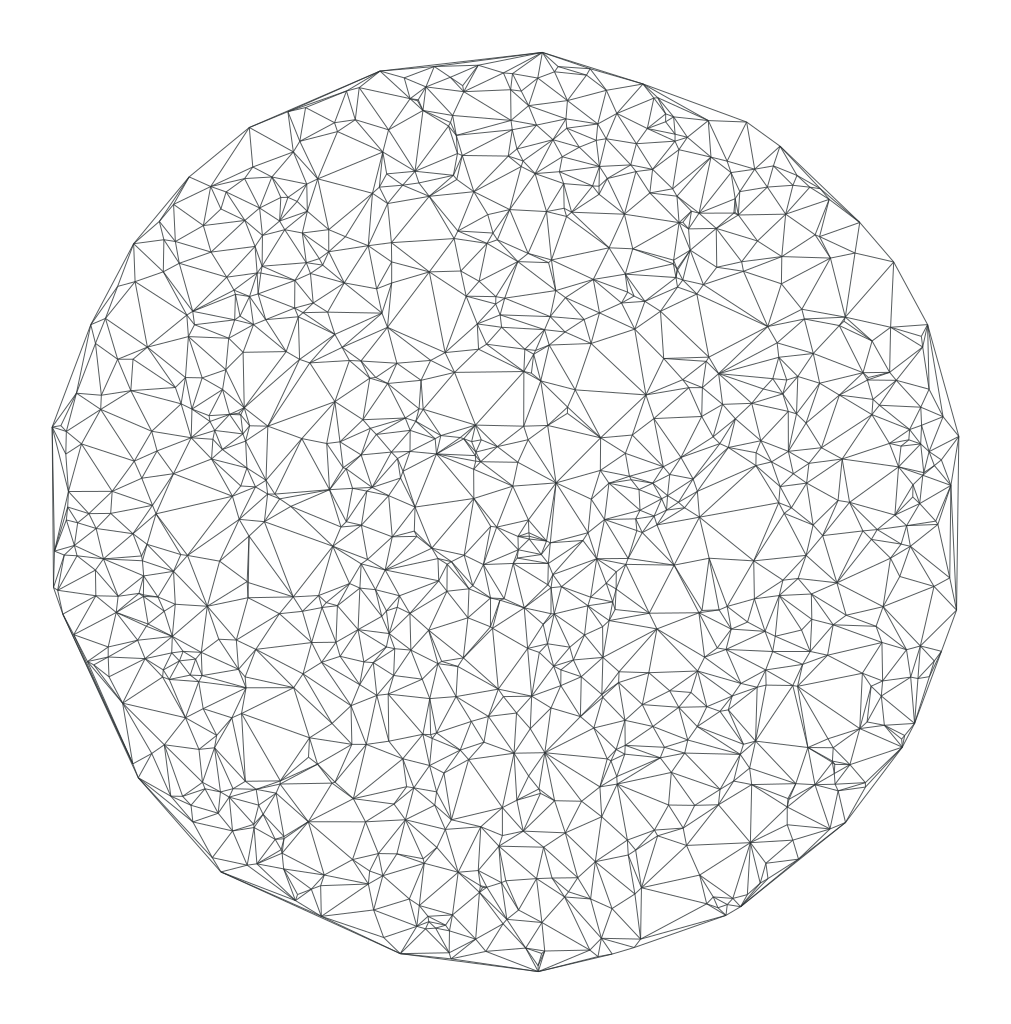
\includegraphics[width=\linewidth]{graphics/delaunay.png}
		\caption{Full Delaunay Triangulation (avg. deg. \(\approx 6\))}
		\label{fig:delaunay_full_viz}
	\end{subfigure}
	\hfill
	\begin{subfigure}{0.3\linewidth}
		\centering
		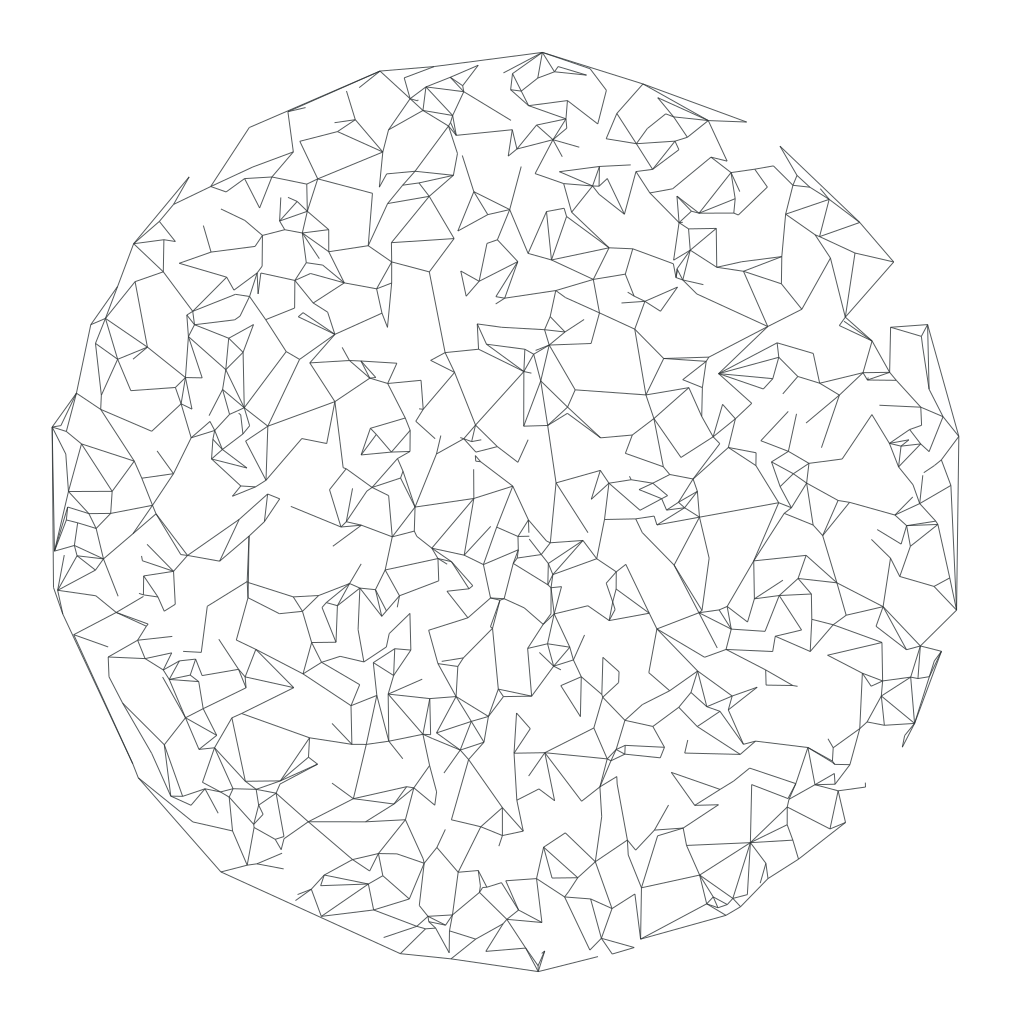
\includegraphics[width=\linewidth]{graphics/delaunay_random_delete.png}
		\caption{Sparse DT (Random Deletion, avg. deg. \(\approx 2.5\))}
		\label{fig:delaunay_random_del_viz}
	\end{subfigure}
	\hfill
	\begin{subfigure}{0.3\linewidth}
		\centering
		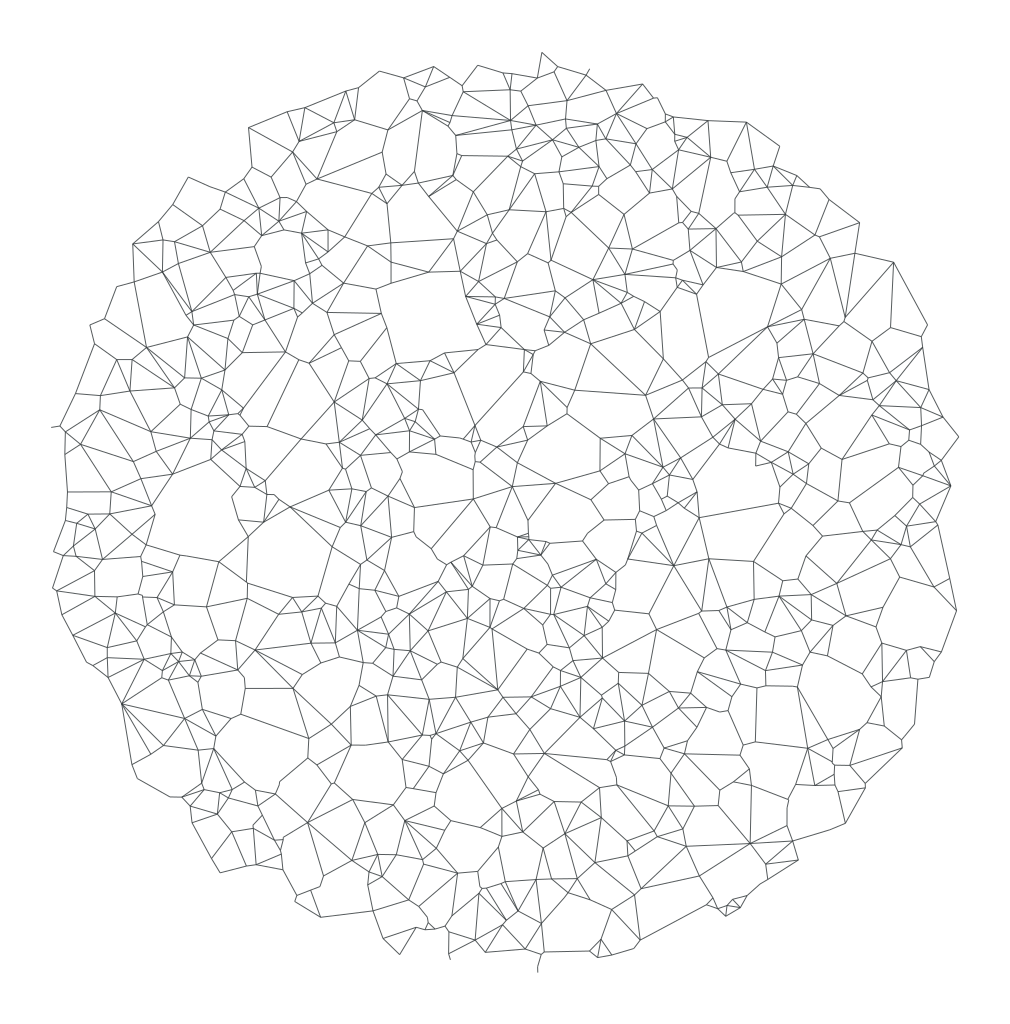
\includegraphics[width=\linewidth]{graphics/gabriel_graph.png}
		\caption{Gabriel Graph (GG)\newline}
		\label{fig:delaunay_gg_viz}
	\end{subfigure}

	\vspace{0.2cm}

	\begin{subfigure}{0.3\linewidth}
		\centering
		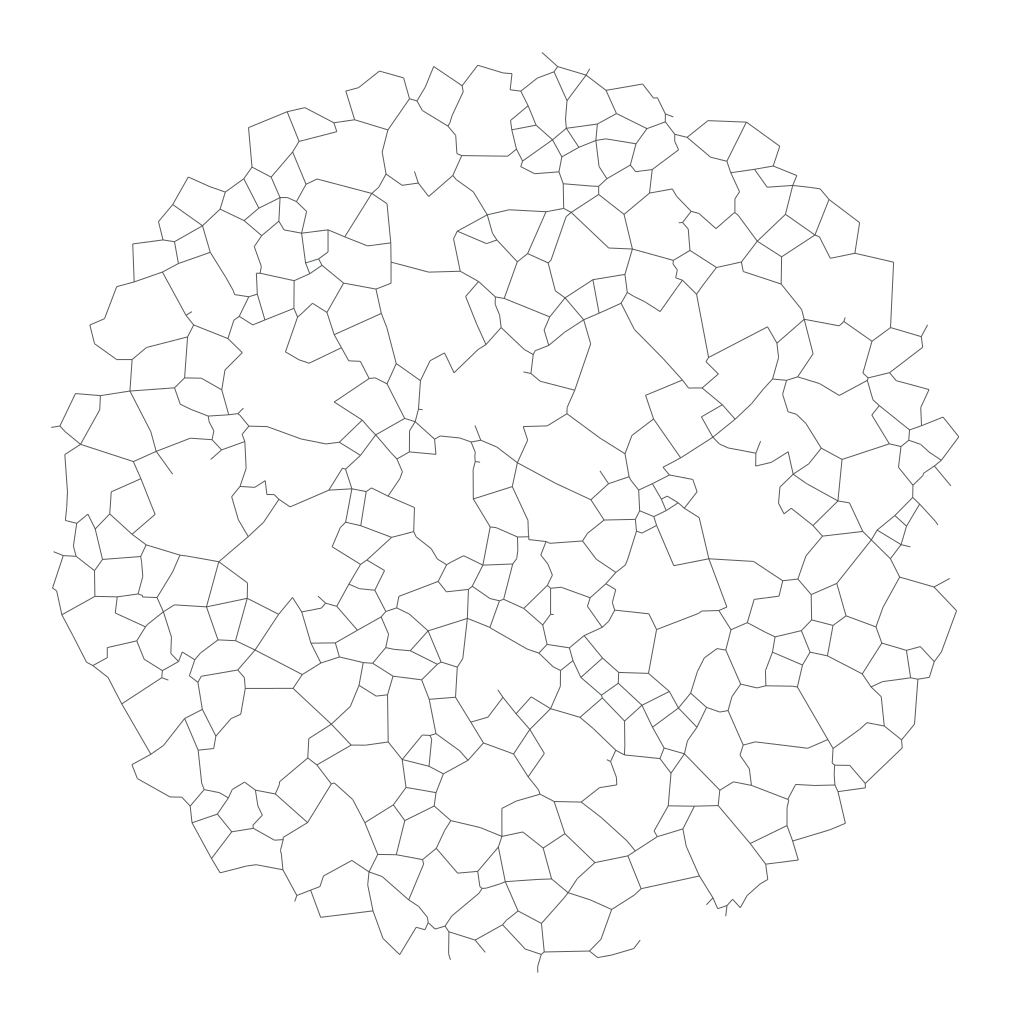
\includegraphics[width=\linewidth]{graphics/relative_neighborhood.png}
		\caption{Relative Neighborhood Graph (RNG)}
		\label{fig:delaunay_rng_viz}
	\end{subfigure}
	\hfill
	\begin{subfigure}{0.6\linewidth}
		\centering
		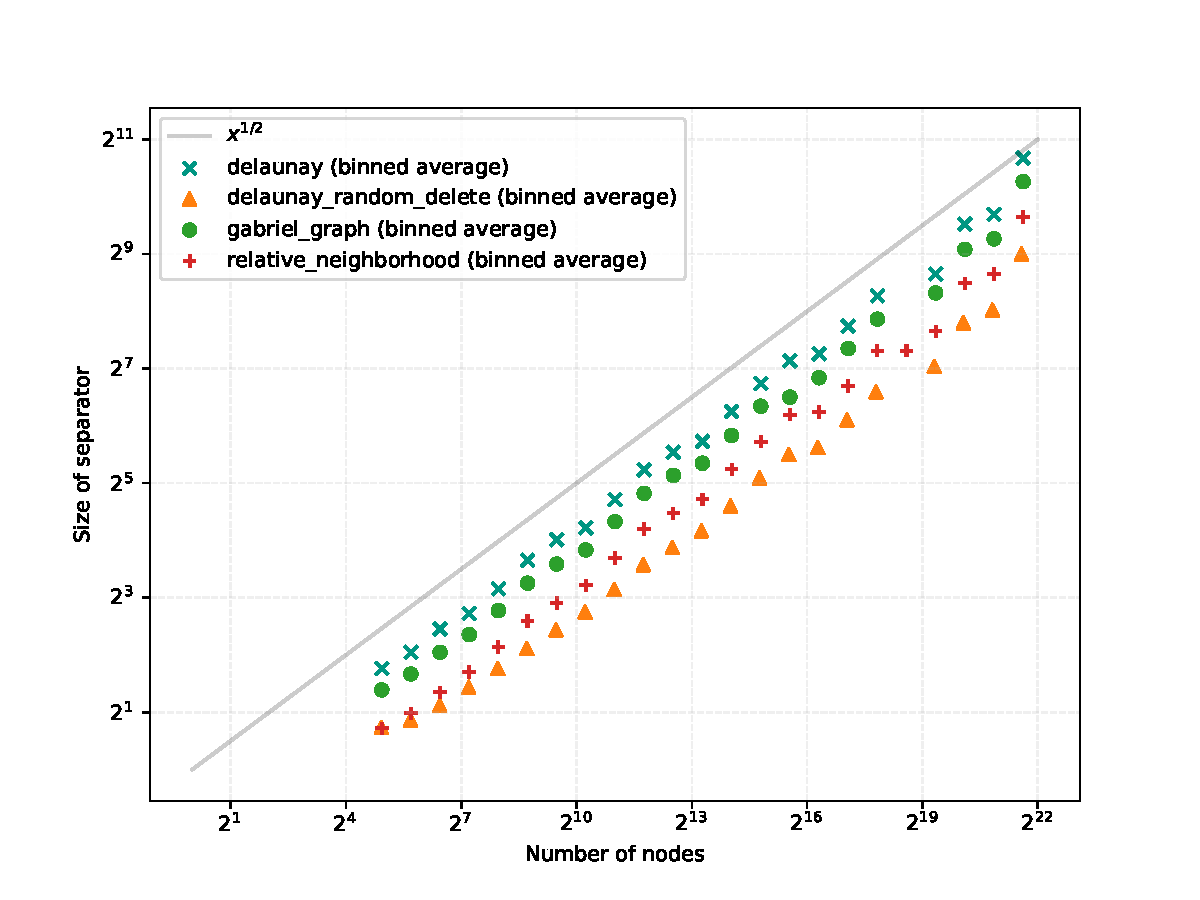
\includegraphics[width=\linewidth]{graphics/delaunay_variants_sep.pdf}
		\caption{Separator scaling for Delaunay variants.}
		\label{fig:delaunay_variants_sep_plot}
	\end{subfigure}
	\caption{Comparison of Delaunay Triangulation and its sparse subgraphs derived from the same point set: visualizations (a-d) and separator scaling (e). Separators were computed using InertialFlowCutter (tests with FlowCutter and KaHIP yielded similar asymptotic scaling).}
	\label{fig:delaunay_variants_comparison}
\end{figure}

% These experiments with sparse grids and various forms of sparse Delaunay triangulations suggest that while combining geometric point generation with methods to achieve low average degree can yield practical separator sizes numerically close to those of road networks (due to potentially small constant factors), the underlying asymptotic scaling remains \bigO{n^{1/2}}.
% This indicates that these standard planar graph models, even when carefully sparsified, do not inherently capture the mechanism leading to the more favorable \(\approx \bigO{n^{0.37}}\) scaling observed in real road networks.

\section{Highway Dimension}
\label{sec:synthetic:highway_dimension}

Given that the simpler graph models explored in previous sections do not reproduce the observed \bigO{n^{1/3}} separator scaling of road networks, we turn our attention to more complex generative processes designed to capture other relevant structural properties.
One such property is highway dimension, introduced by Abraham et al. \cite{abraham_highway_2010}.
Intuitively, a graph possesses a small highway dimension if, for every radius \(r > 0\), there exists a sparse set of vertices \(S_r\) such that every shortest path longer than \(r\) intersects \(S_r\).
A set is considered sparse if every ball of radius \(\mathcal{O}(r)\) contains only a small number of vertices from \(S_r\) \cite{abraham_highway_2010}.
The significance of this property stems from the finding that low highway dimension provides provable performance guarantees for several important route planning algorithms, including REACH \cite{goldberg_reach_2006}, Contraction Hierarchies \cite{geisberger_contraction_2008}, Highway Hierarchies \cite{sanders_highway_2005}, Transit Node Routing \cite{bast_fast_2007}, and SHARC \cite{bauer_sharc_2010}.
The work introducing highway dimension also proposes a synthetic graph generator (henceforth ABR generator) intended to produce graphs exhibiting this property \cite{abraham_highway_2010}.
The generation process, based on the description in \cite{hutchison_synthetic_2010}, operates iteratively.
It begins with an empty graph \( G = (V, E) = (\emptyset, \emptyset) \) and progressively adds new vertices \(v_t\) to \(V\), whose locations in the metric space (in our case a disk in \(\mathbb{R}^2\)) are chosen randomly.
Throughout this process, the generator maintains a series of \(2^i\)-covers, denoted \(C_i\), for each level \(i\) where \(1 \leq i \leq \log D\), and \(D\) represents the diameter of the metric space.
A set \(C_i \subseteq V\) is a \(2^i\)-cover if any two vertices \(u, v \in C_i\) satisfy \(d(u, v) \geq 2^i\), and every vertex \(u \in V\) is within distance \(2^i\) of some vertex in \(C_i\).
When a new vertex \(v_t\) is added, the generator identifies the smallest index \(i\) such that there exists a vertex \(w \in C_i\) with \(d(v_t, w) \leq 2^i\).
The new vertex \(v_t\) is then added to all covers \(C_j\) for which \(0 \leq j < i\).
If no such index \(i\) exists, \(v_t\) is added to all cover sets \(C_j\).
Edges are subsequently added based on these covers and a tuning parameter \(k\).
For each cover \(C_j\) containing \(v_t\) (where \(0 \leq j < i\)), and for each existing vertex \(w \in C_j\), an edge \((w, v_t)\) is added if their distance satisfies \(d(w, v_t) \leq k \cdot 2^j\).
Furthermore, for each \(C_j\) containing \(v_t\) where \(j < \log D\) and \(v_t\) is also present in \(C_{j+1}\), an edge is added connecting \(v_t\) to its nearest neighbor within the set \(C_{j+1}\).
For our experiments, we adopt parameter settings similar to those used by \cite{hutchison_synthetic_2010}, setting the diameter \(D = 2^{25}\) and the connection parameter \(k = \sqrt{2}\).
Bauer et al. also describe an alternative node sampling strategy aimed at creating structures resembling city clusters \cite{hutchison_synthetic_2010}.
We implement and test both the uniform random sampling and this cluster-based sampling approach.
Our experiments indicate no significant difference in the resulting separator sizes between the two sampling methods using the ABR generator framework.
The analysis of graphs generated using the ABR method yields separators that scale approximately as \bigO{n^{1/2}}.
This result is noteworthy because graphs generated by this process are typically highly non-planar.
It serves as a reminder that observing \bigO{n^{1/2}} separator scaling does not necessarily imply planarity.
\Cref{fig:abr_graph_separators} provides a visual example of an ABR-generated graph and illustrates the observed separator scaling.

\begin{figure}[tbhp]
	\centering
	\begin{subfigure}{0.35\linewidth}
		\centering
		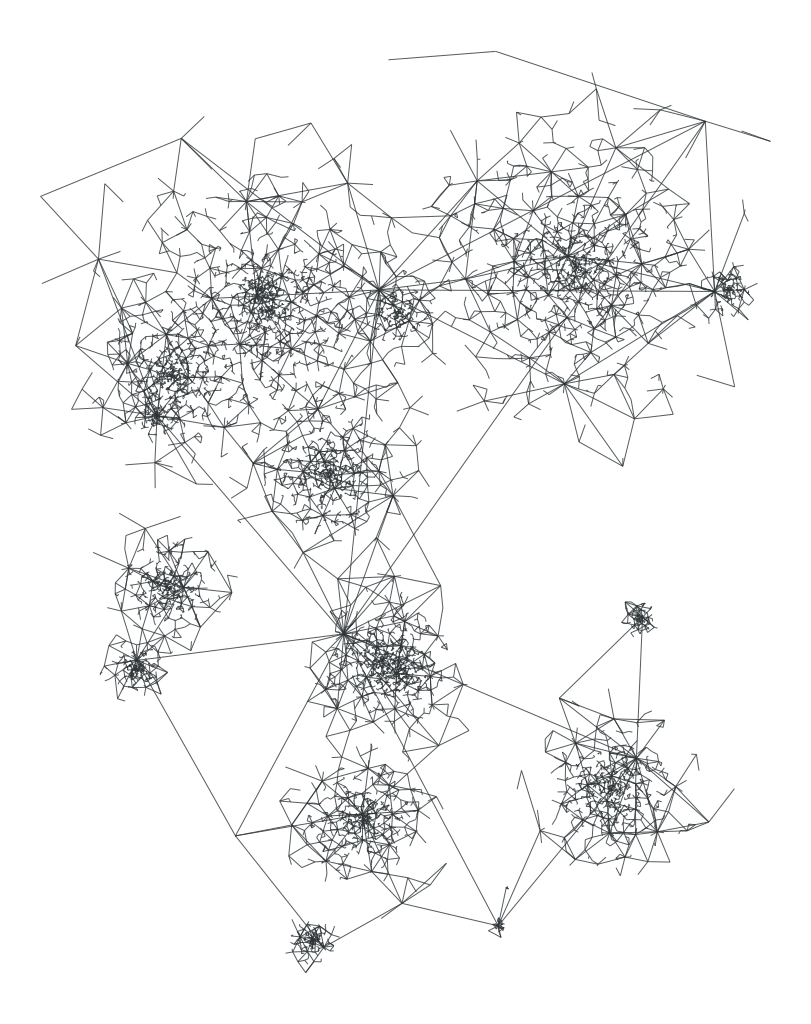
\includegraphics[height=\linewidth, angle=90]{graphics/highway.png}
		\caption{Visualization of a synthetic graph generated using the ABR low highway dimension algorithm with \(10^4\) nodes.}
		\label{fig:abr_graph_viz}
	\end{subfigure}
	\hfill
	\begin{subfigure}{0.55\linewidth}
		\centering
		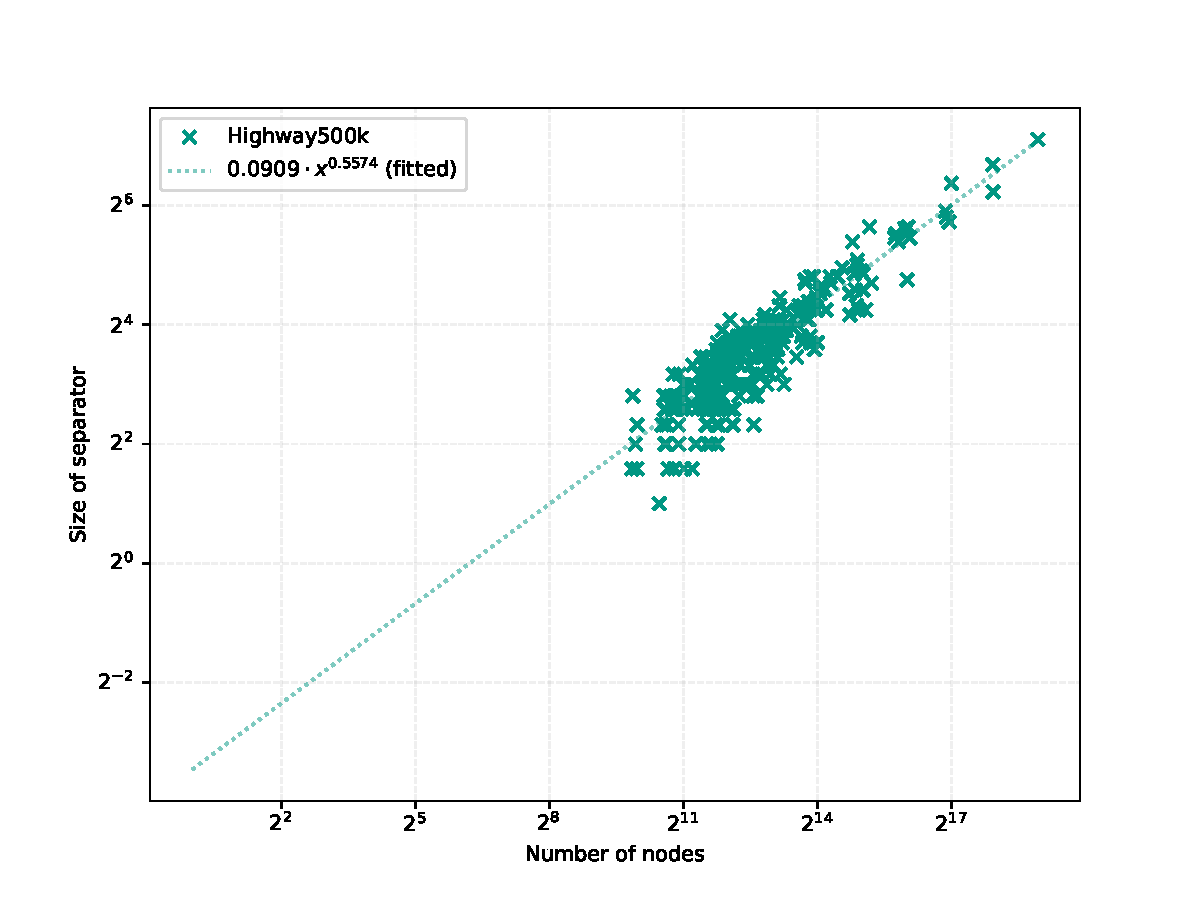
\includegraphics[width=\linewidth]{graphics/sep_highway.pdf}
		\caption{Separator size scaling observed during recursive partitioning of ABR-generated graphs. Separator sizes scale approximately as \bigO{n^{1/2}}. The fit shown excludes subgraphs with \( \le 256 \) vertices due to their disproportionately large separators.}
		\label{fig:abr_graph_sep_plot}
	\end{subfigure}
	\caption{Analysis of synthetic graphs generated using the ABR algorithm \cite{abraham_highway_2010}. Separators were computed using InertialFlowCutter (tests with FlowCutter and KaHIP yielded similar asymptotic scaling).}
	\label{fig:abr_graph_separators}
\end{figure}

\section{Hierarchical Structure}

In the following sections, we explore four distinct approaches to generating synthetic graphs with hierarchical structures.

\subsection{Voronoi-Based Hierarchical Generator}

One approach to generating synthetic networks with hierarchical features follows the method proposed by Bauer et al. \cite{hutchison_synthetic_2010}.
This method utilizes Voronoi diagrams iteratively.
A Voronoi diagram, given a set of points \(P\), partitions the plane into convex regions, where each region contains the area closer to one point in \(P\) than to any other point in \(P\).
The generation process commences within a predefined initial polygon, which defines the spatial extent of the synthetic network.
Points, designated as sites \(P\), are then generated within this polygon according to a chosen sampling strategy.
One strategy involves sampling a specified number of points uniformly at random throughout the polygon's interior.
Alternatively, to better emulate settlement patterns, a clustered sampling approach can be employed.
This approach involves first sampling locations for a number of population centers within the polygon.
Each center is then assigned characteristics, such as a population size or an influence radius, drawn from a chosen distribution.
Subsequently, points are sampled in the vicinity of each city center, concentrated within its influence radius, with the number of points related to the city's size.
Regardless of the sampling method, the resulting set of points \(P\) serves as the input for computing the Voronoi diagram for this initial level.
The Voronoi diagram partitions the polygon into regions based on nearest-neighbor relationships to the points in \(P\).
The edges of this Voronoi diagram (where adjacent regions meet) are then added to the synthetic graph.
The vertices of the graph correspond to the points where 3 or more Voronoi regions meet.
To introduce hierarchy, some of the resulting Voronoi regions (polygons) are selected, and the process is recursively applied within them: new points are sampled inside the selected region (using either uniform or clustered sampling), and a new Voronoi diagram is constructed within its boundaries, adding further edges to the graph.
Phase two of the generation process addresses the density of the graph \(G\) resulting from the Voronoi tessellation by constructing a sparse graph \(t\)-spanner \(H\).
A subgraph \(H\) is a \(t\)-spanner of \(G\) if it preserves all pairwise distances up to a multiplicative factor of \(t\).
The spanner is built using a greedy algorithm that iterates through the edges of \(G\) sorted by non-increasing length (longest first).
An edge \((u, v)\) with length \(len(u, v)\) is added to the spanner \(H\) only if the current shortest path distance between \(u\) and \(v\) within \(H\), denoted \(dist_H(u, v)\), is greater than \(t \cdot len(u, v)\).
To compute \(dist_H(u, v)\), Dijkstra's algorithm is employed.
Additionally, a union-find data structure maintains the connected components of \(H\), allowing for immediate addition of edges connecting previously disconnected vertices.
Bauer et al. propose processing edges in non-increasing order (longest first) as a heuristic primarily intended to improve the computational efficiency of the spanner construction,
the idea is to handle long edges while the intermediate spanner graph \(H\) is still sparse, potentially speeding up distance computations \cite{hutchison_synthetic_2010}.
For completeness, we briefly mention an alternative pruning strategy for a different generative model that will be detailed in a later section (\cref{sec:hierarchical_delaunay_generation}).
This method tends to produce graphs with greater visual resemblance to real-world road networks than the Bauer et al. approach, though this comes at a higher computational cost.

This generation method introduces artifacts.
For example, connections between major structures defined at higher levels (like large "cities") might be unrealistically sparse, potentially consisting of only a few edges.
Another artifact is that higher-level Voronoi edges (e.g., "highways" separating major regions) act as hard boundaries that lower-level edges (within regions) often do not cross, creating unrealistically effective separators along these top-level edges.
Analyzing separators in the final sparse graphs generated by this Voronoi-based method reveals interesting characteristics related to the hierarchy.
Plots of separator size versus subgraph size often exhibit noticeable local minima, which appear to correspond to the transitions between the hierarchical layers created during generation.
This can lead to separators of approximately constant size when partitioning cuts primarily occur between these major structures at layer intersections.
Within a single layer generated by the Voronoi tessellation (before sparsification), the separators tend to exhibit scaling closer to \bigO{n^{1/2}}.
Consequently, if the recursion depth is limited and the highest-level structures are allowed to grow large, their \bigO{n^{1/2}} separator behavior will dominate the separator size scaling.
\Cref{fig:voronoi_hierarchy} illustrates the structure and separator behavior of the final sparse graph.

\begin{figure}[tbhp]
	\centering
	\begin{subfigure}{0.35\linewidth}
		\centering
		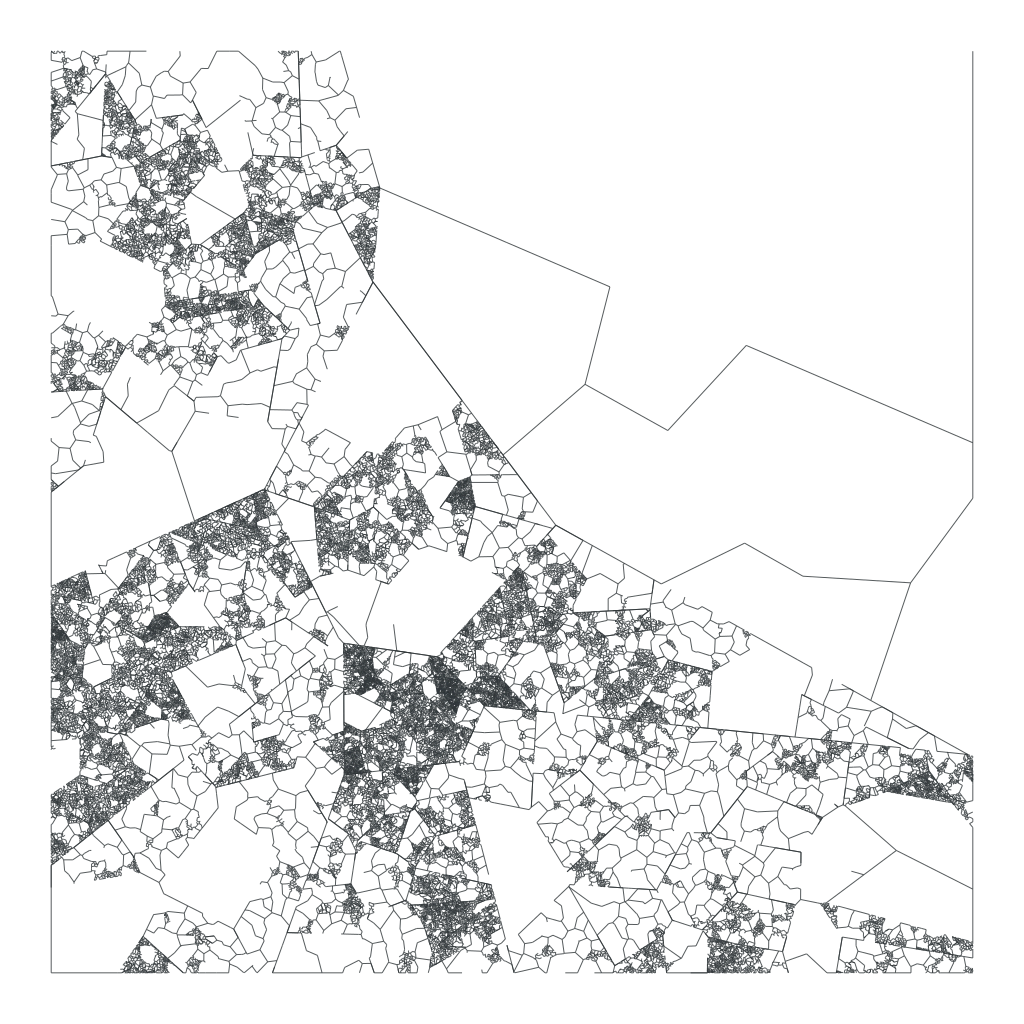
\includegraphics[width=\linewidth]{graphics/voronoi.png}
		\caption{Visualization of a synthetic graph generated using the Voronoi method.}
		\label{fig:voronoi_hierarchy_viz}
	\end{subfigure}
	\hfill
	\begin{subfigure}{0.55\linewidth}
		\centering
		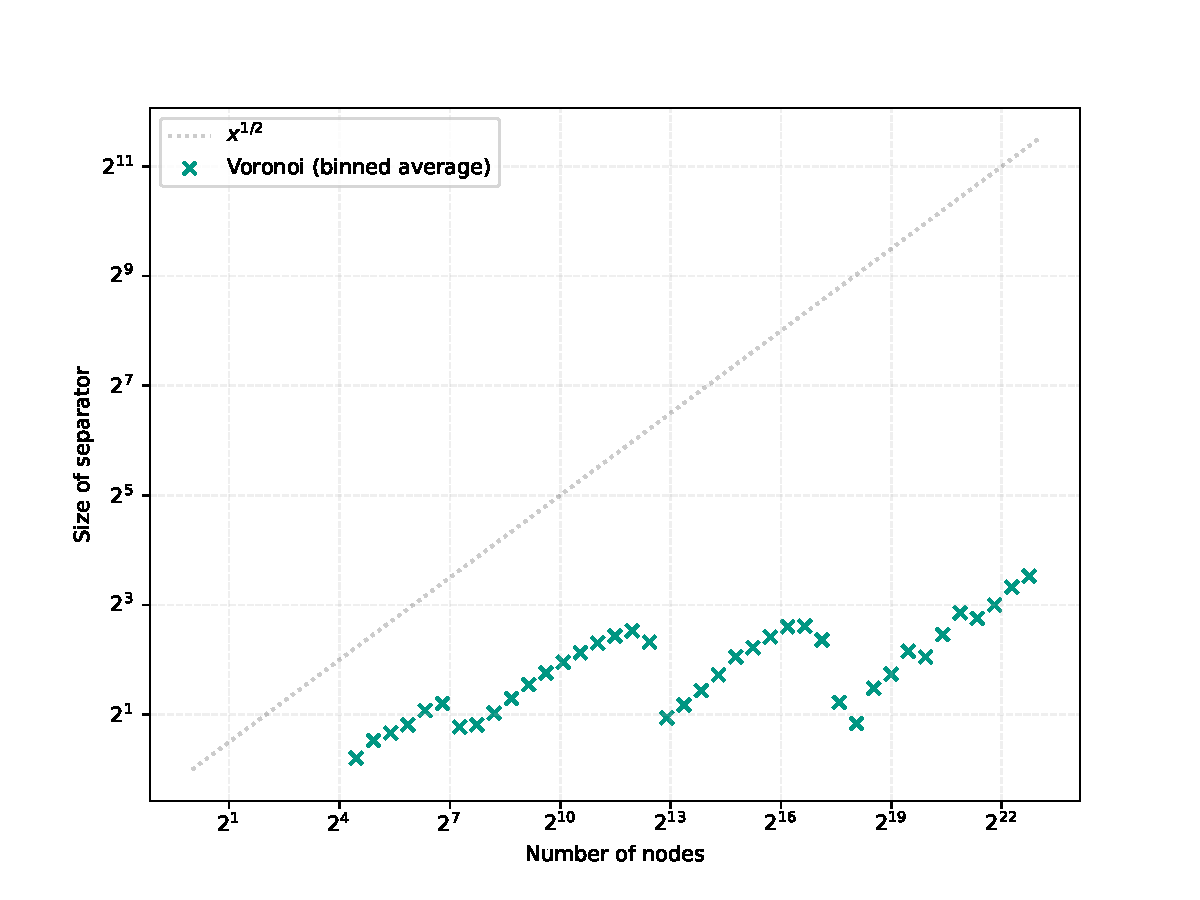
\includegraphics[width=\linewidth]{graphics/sep-voronoi.pdf}
		\caption{Separator size scaling for the hierarchical Voronoi graph, showing local minima at layer transitions.}
		\label{fig:voronoi_hierarchy_sep_plot}
	\end{subfigure}
	\caption{Analysis of synthetic graphs generated using the hierarchical Voronoi approach from Bauer et al. \cite{hutchison_synthetic_2010}. Separators were computed using InertialFlowCutter (tests with FlowCutter and KaHIP yielded similar asymptotic scaling).}
	\label{fig:voronoi_hierarchy}
\end{figure}

\subsection{Nested Grids}

To explore hierarchical effects in a more controlled manner, we also investigate a simpler but conceptually related approach using nested grids.
This method aims to construct a hierarchical graph by recursively embedding grid graphs within the cells of a parent grid, potentially allowing us to deliberately engineer specific separator scaling properties.
The fundamental idea is recursive: a level-1 structure is a standard square grid.
A level-\(i\) nested grid (for \(i > 1\)) is then constructed from a higher-level parent grid where selected cells are replaced by entire instances of level-\(i-1\) nested grids.
This process can be repeated for any number of layers, creating a fractal-like structure of grids within grids.
An optional refinement can be applied to make the graph sparser by removing redundant edges from parent grids.
An edge of a parent grid is considered redundant if the cell it borders has a subgraph embedded within it.
This is because the boundary of the embedded subgraph provides a new, more detailed path between the endpoints of the parent grid edge.
Removing these \enquote{overlapped} parent edges reduces the graph's overall edge density slightly without altering its asymptotic separator scaling.
\cref{fig:nested_grid_analysis} shows a small conceptual example of a nested grid with four layers.

\begin{figure}[tbhp]
	\centering
	\begin{subfigure}{0.35\linewidth}
		\centering
		\includegraphics[width=\linewidth]{graphics/nestedgrid.pdf}
		\caption{Conceptual illustration of a simple nested grid structure with four hierarchical levels.}
		\label{fig:nested_grid_viz}
	\end{subfigure}
	\hfill
	\begin{subfigure}{0.55\linewidth}
		\centering
		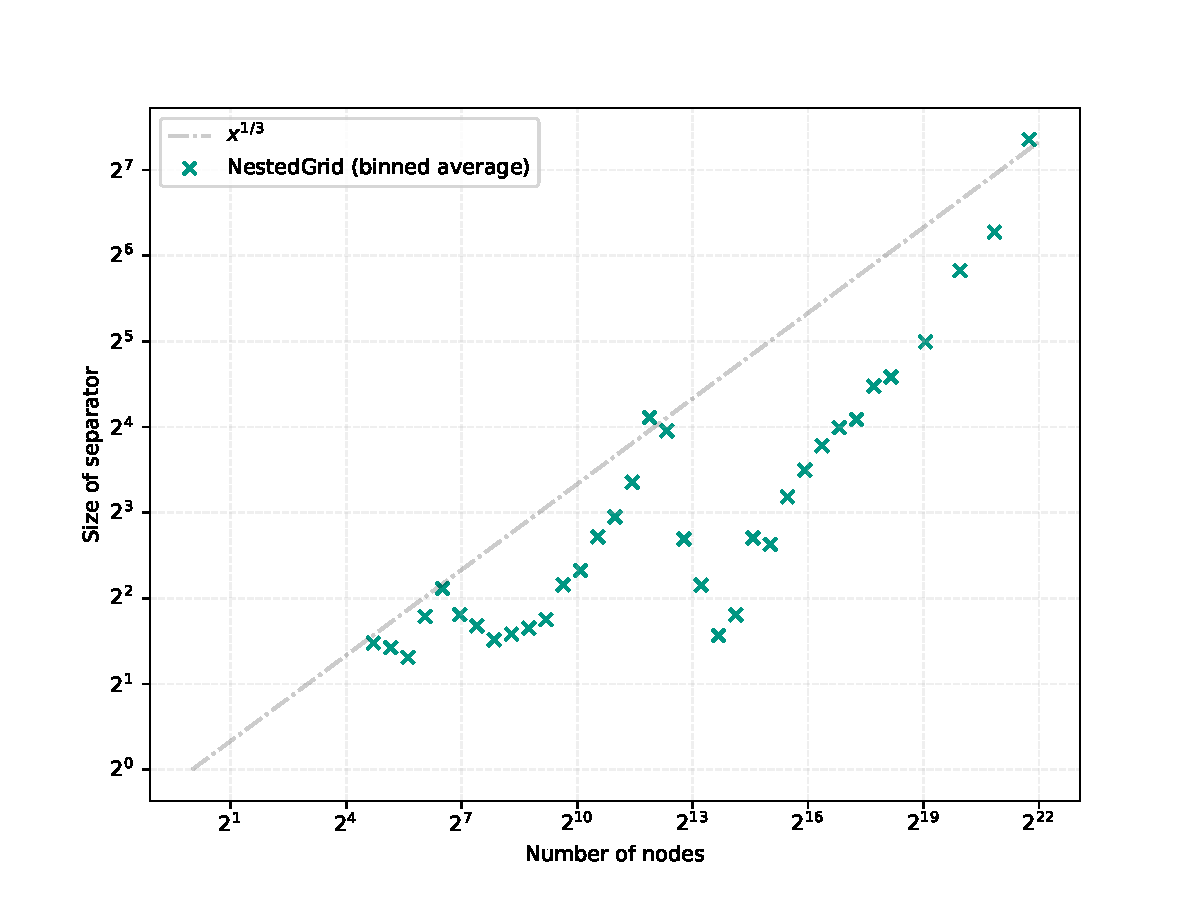
\includegraphics[width=\linewidth]{graphics/sep-nestedgrid.pdf}
		\caption{Separator size scaling for nested grids, showing pronounced local minima.}
		\label{fig:nested_grid_sep_plot}
	\end{subfigure}
	\caption{Analysis of synthetic graphs generated using the nested grid approach. Separators were computed using InertialFlowCutter (tests with FlowCutter and KaHIP yielded similar asymptotic scaling).}
	\label{fig:nested_grid_analysis}
\end{figure}

A nested grid construction with \(L\) layers is determined by \(L\) grid sizes (specifying the dimensions of the grid at each layer) and \(L-1\) placement parameters (specifying how many subgraphs from layer \(i+1\) are placed within layer \(i\)).
This parameterization offers the possibility of attempting to enforce a target separator scaling, such as \bigO{n^{1/3}}, by carefully choosing the parameters at each level transition.
We assume that separating the nested structure primarily involves cutting through the top-level grid structure.
If the number of embedded subgraphs is not excessively large, the separator size might be approximated by the width \(w\) of the top-level grid, similar to a standard grid separator.
We can estimate the total number of vertices of a subgraph of the nested grid strucutre \(V_\text{sub}\) based on the top level grid width \(w\) of the current layer, the number \(k\) of subgraphs placed within its cells, and the size \(s\) of each subgraph:
\[ |V_\text{sub}| \approx w^2 + k \cdot s \]
This estimate is approximate as it may double-count vertices along the boundaries where subgraphs connect to the parent grid.
The estimate also assumes we are only looking at perfect nested grids, which is not true as we are looking at general subgraphs from a nested dissection.
To enforce \bigO{n^{1/3}} scaling specifically at this layer transition, we can equate the separator size (approximated by \(w\)) with \(|V_\text{sub}|^{1/3}\):
\[ w \approx (|V_\text{sub}|)^{1/3} \approx (w^2 + ks)^{1/3} \]
This leads to the cubic equation \( w^3 - w^2 - ks = 0 \).
If we fix the subgraph count \(k\) and subgraph size \(s\), we can solve for the grid width \(w\) required to satisfy this condition at the transition.
One root of this cubic equation for \(w\) is given by:
\[ w = \frac{(27 k s + \sqrt{(27 k s + 2)^2 - 4} + 2)^{1/3}}{3 \cdot 2^{1/3}} + \frac{2^{1/3}}{3 (27 k s + \sqrt{(27 k s + 2)^2 - 4} + 2)^{1/3}} + \frac{1}{3} \]

By carefully selecting \(w\) based on \(k\) and \(s\) using this relationship at each hierarchical level, one can attempt to construct a graph where the separator size scales roughly as the cube root of the number of nodes at each layer transition.
This controlled approach allows the local minima in separator sizes, already seen in the Voronoi method, to be made more pronounced and regular, as all subgraphs at a given level transition can be designed with the same size \(s\).
However, achieving a consistent overall \bigO{n^{1/3}} scaling for the entire graph across all sizes \(n\) remains a challenge.
The observed local minima in separator size occur systematically at the transitions between hierarchical levels.
This is because the construction method inherently creates sparse connections between components defined at different levels.
\cref{fig:nested_grid_connectivity_example} provides a simplified illustration of this principle, showing two example components from the same levels within the hierarchy, not the entire structure of a layer.
In this specific illustration, the components (represented by nodes 1-4 and 5-8) are linked only by the edges (3,5) and (4,6).
Consequently, removing just one endpoint from each connecting edge suffices to disconnect them.
This demonstrates how a vertex separator of small, constant size (size 2) exists between levels, regardless of the internal size of the components themselves.
Such constant-size separators at every level transition are the underlying cause of the pronounced local minima observed in the separator scaling plots for these nested structures.

\begin{figure}[tbhp]
	\centering
	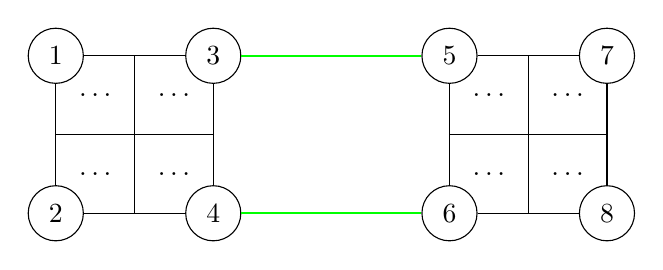
\begin{tikzpicture}[every node/.style={draw, circle, minimum size=0.7cm}]
		\node (1) at (0,2) {1};
		\node (2) at (0,0) {2};
		\node (3) at (2,2) {3};
		\node (4) at (2,0) {4};

		\node (5) at (5,2) {5};
		\node (6) at (5,0) {6};
		\node (7) at (7,2) {7};
		\node (8) at (7,0) {8};

		\draw (1) -- (2) -- (4) -- (3) -- (1);
		\draw (5) -- (7) -- (8) -- (6) -- (5);

		\draw[color=green, thick] (3) -- (5);
		\draw[color=green, thick] (4) -- (6);
		\draw (1,1) -- (1,0);
		\draw (1,1) -- (1,2);
		\draw (1,1) -- (0,1);
		\draw (1,1) -- (2,1);

		\draw (6,1) -- (5,1);
		\draw (6,1) -- (6,0);
		\draw (6,1) -- (6,2);
		\draw (6,1) -- (7,1);

		\node[draw=none] at (0.5,0.5) {\(\dots\)};
		\node[draw=none] at (1.5,0.5) {\(\dots\)};
		\node[draw=none] at (1.5,1.5) {\(\dots\)};
		\node[draw=none] at (0.5,1.5) {\(\dots\)};

		\node[draw=none] at (5.5,0.5) {\(\dots\)};
		\node[draw=none] at (6.5,0.5) {\(\dots\)};
		\node[draw=none] at (6.5,1.5) {\(\dots\)};
		\node[draw=none] at (5.5,1.5) {\(\dots\)};
	\end{tikzpicture}
	\caption{Simplified illustration of connectivity between components from adjacent hierarchical levels. The components (nodes 1-4 and 5-8) are connected only by the two green edges (3,5) and (4,6). Removing one endpoint from each edge (e.g., 3 and 6) forms a size-2 vertex separator, irrespective of component sizes.}
	\label{fig:nested_grid_connectivity_example}
\end{figure}









\subsection{Hierarchical Delaunay Graph Generation}
\label{sec:hierarchical_delaunay_generation}

Our efforts to generate synthetic graphs with realistic road network properties, particularly small separators, led us to refine techniques inspired by prior work on synthetic road network generation, such as that of Bauer et al.
\cite{hutchison_synthetic_2010}.
A significant artifact observed in some Voronoi-based hierarchical models was that major transport arteries, analogous to motorways, could not be realistically crossed by lower-level roads.
This limitation arose because new expansion sites were generated strictly within the polygonal cells defined by the higher-level Voronoi tessellation, effectively making top-level Voronoi edges hard boundaries.
Our revised core idea allows new centers of expansion to emerge from the existing network infrastructure itself.
Thus, new expansion sites are selected from the nodes of the current graph structure rather than from within predefined areal polygons.

\paragraph{Initial Approach}

An initial concept explored an iterative Delaunay approach.
This process would commence with a Delaunay triangulation of an initial point set.
In subsequent hierarchical levels, a subset of existing points would be selected as \emph{expansion sites}.
New points would then be sampled in the vicinity of each of these sites.
Following this, a new Delaunay triangulation would be performed independently for each expansion site.
This iterative process is designed to emulate a self-reinforcing concentration dynamic, which is analogous to preferential attachment models.
The rationale is to replicate how real-world settlement and infrastructure patterns evolve, where new growth is more likely to occur in or around already dense regions.
By making points in these areas more probable candidates for subsequent expansion, the model naturally gives rise to a hierarchical landscape of concentrated clusters, mimicking the formation of urban centers.
This recursive generation would continue for a specified number of levels.
The result at this stage is a collection of disjoint, small, triangulated graphs embedded in the plane, whose edge lengths differ significantly based on the geometric scale at which they were generated.
As a final step, a planarization process, as described in \cref{alg:planarization}, is applied: edges, interpreted as straight line segments, are checked for intersections.
Any intersections found are resolved by introducing new vertices at these points and subdividing the original edges accordingly, thus making the graph connected and planar.
This method showed initial promise in creating structures that could yield separators with scaling behavior similar to that of road networks.

\paragraph{Refined Generation}

Building upon insights from this strategy, we developed a more streamlined and effective method, which is the primary focus of this section.
Instead of performing Delaunay triangulations at each hierarchical level followed by a final planarization step, we first generate the complete set of points across all desired levels.
Only after all points have been generated is a single, global Delaunay triangulation performed on the entire final point set.
The pseudocode for this hierarchical Delaunay generation process is detailed in \cref{alg:hierarchical_delaunay}.
The method \texttt{uniformRandomPointsInCircle(center, radius, k)} samples \(k\) points uniformly at random within a circle of given radius centered at the specified point.
A deliberate design choice in our hierarchical point generation process (\cref{alg:hierarchical_delaunay}) is that candidates for new expansion sites at each level \(i\) are selected from the entire set of currently existing points \(P\), rather than exclusively from points generated in the immediately preceding level \(i-1\).
This approach reflects the real-world phenomenon where new settlements, even smaller ones, can emerge around and connect to established, major infrastructure hubs that might have formed at much earlier stages of network growth,
for instance, a small town developing near a major motorway interchange.
We also experimented with an alternative strategy where expansion sites for a given level were chosen only from the points generated in the previous level.
However, this restriction did not yield any noticeable differences in the overall structural properties or separator characteristics of the resulting graphs.
\begin{algorithm}[tbhp]
	\Input{Number of hierarchical levels \(L\), \\
		Level expansion fractions \(f_i\) (where \(f_1 = 1.0\)), \\
		Points to generate per expansion site \(k_i\), \\
		Expansion radii \(r_i\), \\
		for \(1 \le i \le L\)}
	\Output{Geometric graph \(G\)}
	\BlankLine
	\(P \longleftarrow \{p_\text{random}\}\)\;
	\BlankLine
	\ForAll{\(i \in [1, L]\)}{
		\(C_i \longleftarrow\) P.chooseRandom(\(\left\lfloor f_i \cdot |P|\right\rfloor\))\;
		\ForAll{center \(\in C_i\)}{
			\(P \longleftarrow P~\cup\) uniformRandomPointsInCircle(center, \(r_i\), \(k_i\))\;
		}
	}
	\BlankLine
	\(G \longleftarrow\) delaunay(\(P\))\;
	pruneEdges(\(G\))\;
	\Return{\(G\)}\;
	\caption{Hierarchical Delaunay Graph Generation}
	\label{alg:hierarchical_delaunay}
\end{algorithm}

\paragraph{Pruning}
\label{sec:synthetic:hierarchical_delaunay:pruning}


Analogous to the Delaunay triangulation approach in \cref{sec:synthetic:delaunay_variants}, the global Delaunay triangulation performed in \cref{alg:hierarchical_delaunay} results in a graph with an average vertex degree of approximately 6, which is denser than typical road networks.
To better emulate the characteristics of real road networks, such as an average degree around \(2.5\) and fewer nodes with very high degrees, we apply an edge pruning step.
While Bauer et al. \cite{hutchison_synthetic_2010} also suggested a pruning methodology, we adopt a different strategy tailored to our generated graph structures.
In our approach, edges are considered in order of increasing Euclidean length (shortest first).
An edge \((u,v)\) is removed if the length of the shortest path between its endpoints in the remaining graph does not exceed its original direct length by more than a factor of \(\alpha\), i.e. if \( \text{dist}_{G \setminus \{(u,v)\}}(u,v) \le \alpha \cdot \text{length}(u,v) \).
This edge removal criterion approximates economic viability considerations, as connections that offer marginal utility or are largely redundant would likely not be constructed in real-world road networks.
Through experimentation, we found that a pruning parameter of \(\alpha = 2.5\) effectively reduces the average degree to the target range comparable to that of road networks.
The pseudocode for this edge pruning process is given in \cref{alg:prune_edges}.
A visual comparison of graph structures before and after pruning is provided in \cref{fig:delaunay_vs_no_pruning_graph}.
\begin{algorithm}[tbhp]
	\Input{Graph \(G=(V, E)\), \\
		Pruning parameter \(\alpha\)}
	\Output{Pruned version of \(G\)}
	\BlankLine
	\ForAll{\((u, v) \in E\) sorted by increasing length}{
		\If{\(\text{dist}_{G \setminus \{(u,v)\}}(u, v) \le \alpha \cdot \text{length}(u, v)\)}{
			\(G \longleftarrow G \setminus \{(u, v)\}\)\;
		}
	}
	\caption{Edge pruning based on path length redundancy.}
	\label{alg:prune_edges}
\end{algorithm}

\begin{figure}[tbhp]
	\centering
	\begin{subfigure}{0.45\linewidth}
		\centering
		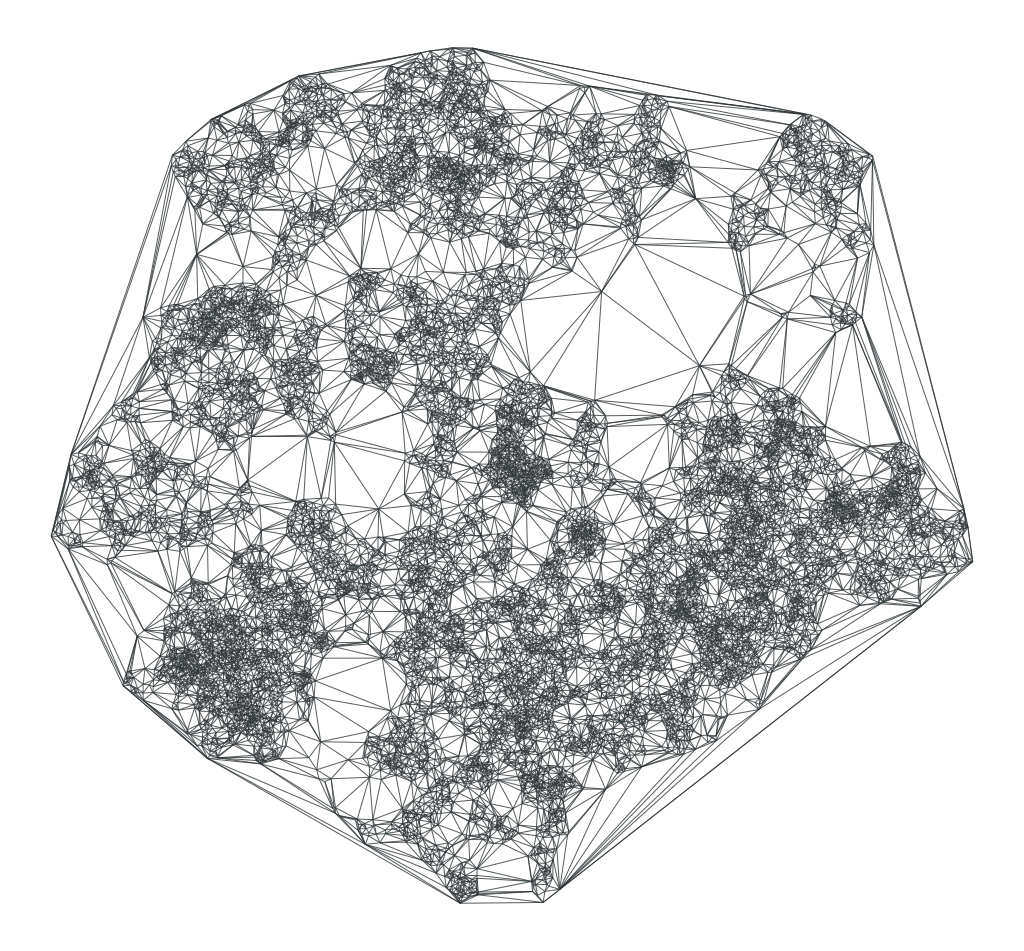
\includegraphics[width=\linewidth]{graphics/delaunay_pre_prune.png}
		\caption{Graph structure before pruning.}
		\label{fig:delaunay_pre_prune_viz}
	\end{subfigure}
	\hfill
	\begin{subfigure}{0.45\linewidth}
		\centering
		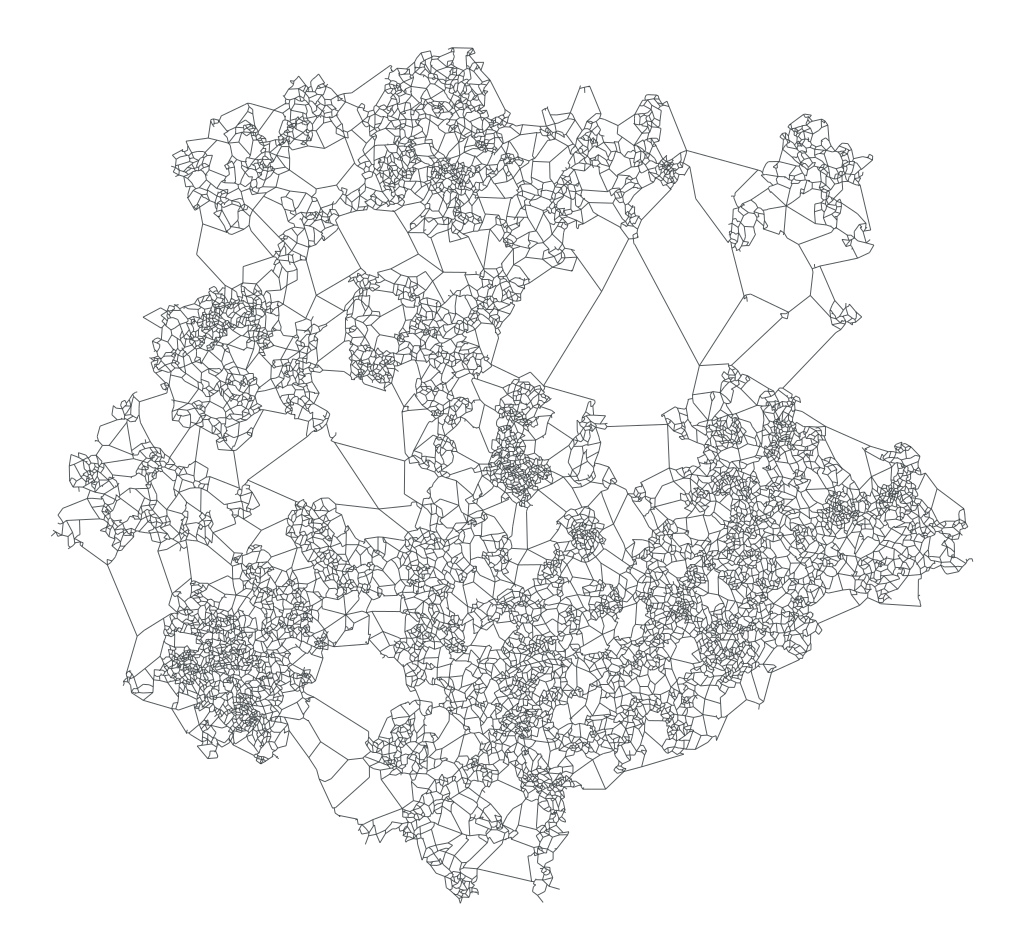
\includegraphics[width=\linewidth]{graphics/delaunay_post_prune.png}
		\caption{Graph structure after pruning.}
		\label{fig:delaunay_post_prune_viz}
	\end{subfigure}
	\caption{Visual comparison of a hierarchical Delaunay graph before and after edge pruning.}
	\label{fig:delaunay_vs_no_pruning_graph}
\end{figure}

The pruning step, while beneficial for achieving a target average degree and a more realistic degree distribution, does not fundamentally alter the asymptotic separator scaling of the generated Delaunay graphs.
\Cref{fig:delaunay_pruned_vs_pre_pruned_sep} illustrates that the separator size scaling remains similar for both pruned and unpruned graphs.

\begin{figure}[tbhp]
	\centering
	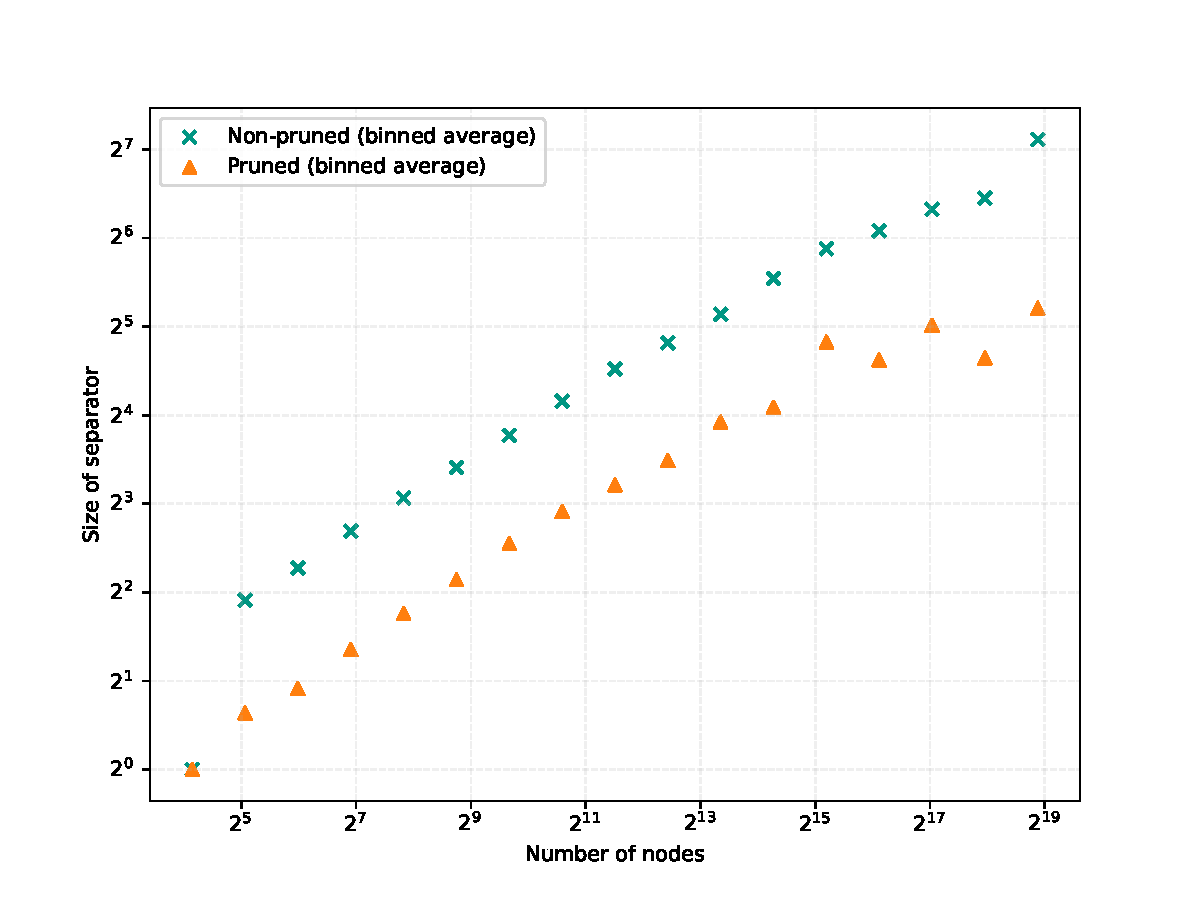
\includegraphics[width=0.7\linewidth]{graphics/delaunay_pre_post_pruning_sep_size.pdf}
	\caption{Comparison of separator size scaling in hierarchical Delaunay graphs before and after the pruning step. Separators were computed using InertialFlowCutter (tests with FlowCutter and KaHIP yielded similar asymptotic scaling).}
	\label{fig:delaunay_pruned_vs_pre_pruned_sep}
\end{figure}

Given that sequential pruning can be computationally intensive due to numerous shortest path computations (typically Dijkstra's algorithm, where path precomputation is infeasible as the graph changes), we also explored an approximate parallel version.
In this variant, instead of looking at edges one by one, we process the edges in the same order as before, but in chunks of size corresponding to the number of available processing threads.
While this approach does not reduce the overall computational complexity, it allows the workload to be distributed across multiple threads.
Shortest path computations for all candidate edges within a chunk are performed in parallel, based on the graph state \emph{before} any edges in that chunk are removed.
After all checks for the current chunk are complete, the identified edges are removed simultaneously.
This parallelization introduces an approximation: an edge \((u,v)\) might be removed because its shortest alternative path relied on another edge \((x,y)\) from the same chunk, which is also concurrently identified for removal.
If \((x,y)\) is removed, the true shortest path for \((u,v)\) in the updated graph might have become longer than the \(\alpha \cdot \text{length}(u,v)\) threshold, but this would not be detected as the checks were based on the graph state at the beginning of the chunk processing.
In extreme cases, this could even lead to the graph becoming disconnected.
Despite this potential for over-pruning, our empirical results suggest that this approximation has a negligible impact on the final graph structure and its properties.
This outcome is likely because edges are sorted by length before being chunked,
thus, edges within a single chunk are often spatially distributed across the graph rather than being highly locally interdependent, minimizing negative interference from concurrent removals.

\paragraph{Parameterization}

The number of hierarchical layers, denoted \(L\), is a key parameter for the generation process detailed in \cref{alg:hierarchical_delaunay}.
Similar to Bauer et al., we also found \(L=4\) to be a suitable choice for generating graphs with realistic road network properties \cite{hutchison_synthetic_2010}.
For \(L=4\), the algorithm requires parameters for level expansion fractions \(f_i\), points per expansion site \(k_i\), and expansion radii \(r_i\), for \(i \in [1, L]\), totaling \(3L\) (i.e., 12 for \(L=4\)) parameters.
However, the effective number of free parameters is lower.
The specific value of the first expansion radius, \(r_1\), primarily scales the entire embedding without fundamentally altering its topological structure, effectively reducing the count to 11 if \(r_1\) is fixed or normalized.
Furthermore, the algorithm specifies that the first level expansion fraction \(f_1 = 1.0\) (ensuring the initial point always seeds the first level of expansion), reducing the free parameters to 10.
If a target total number of vertices, \(n_{\text{target}}\), is desired, one additional parameter (e.g., \(k_L\)) can be adjusted to meet this target, potentially leaving 9 free parameters for a 4-layer model.
The total number of points after level \(j\), denoted \(n_j\) (where \(n_0=1\) is the initial seed point, so \(n_1 = k_1 + 1\) represents the total points after the first expansion), is given by the recurrence relation:
\[
	n_j =
	\begin{cases}
		k_1 + 1                               & \text{if } j=1                        \\
		n_{j-1} + n_{j-1} \cdot f_j \cdot k_j & \text{if } j > 1 \text{ and } j \le L
	\end{cases}
\]
For example, for a 4-layer generation (\(L=4\)), the total number of points \(n_4\) is calculated iteratively:
\begin{align*}
	n_1 & = k_1 + 1                       \\
	n_2 & = n_1 + n_1 \cdot f_2 \cdot k_2 \\
	n_3 & = n_2 + n_2 \cdot f_3 \cdot k_3 \\
	n_4 & = n_3 + n_3 \cdot f_4 \cdot k_4
\end{align*}
The final graph size is thus \(n_L\).

\paragraph{Parameter Interplay and Heuristics for Separator Properties}

Achieving road network-like separator scaling with the hierarchical Delaunay generator involves a nuanced interplay between the expansion fractions \(f_i\), points per site \(k_i\), and expansion radii \(r_i\).
A critical aspect for developing well-behaved separators appears to be ensuring sufficient interaction or \emph{overlap} between regions expanded from different sites.
This helps to avoid overly simplistic connections between hierarchical components, which can lead to pronounced local minima in separator scaling plots.
We observe that decreasing expansion radii \(r_i\) contributes to desirable separator properties.
The median edge length in a Delaunay triangulation of \(n\) uniformly random points within a region of radius \(r\) scales as \bigTheta{r \cdot n^{-1/2}}.
In order for the nested structures to contribute to geometric locality the radii \(r_i\) should also decrease in a similar manner to approximate the median edge length.
For example, constant radii would not yield any geometric locality and points would look uniformly distributed, fading out towards the edge of the graph.
Our empirical observations suggested that without an exponential decrease in radii across levels, achieving consistently small separators is not possible.
However, if radii become too small too quickly, the graph might develop insufficient connectivity between clusters originating from different parent sites.
Consider a thought experiment: if each expansion site has an infinitesimally small influence radius for generating points for the next level, these new points primarily connect among themselves and back to their parent site from the higher level.
The number of points on the effective \enquote{perimeter} of such an expanded site (those able to connect to other, distant parts of the graph) may grow much more slowly than the number of points generated internally, thereby keeping its external connectivity limited,
this effect is amplified by the hierarchical sampling which tends to concentrate points internally.
In such a scenario, one might find a separator for the graph defined by the top-level points (e.g., \(n_1\) points after the first level) with a size scaling as \bigOSmall{n_1^{1/2}}.
If each of these top-level separator nodes is a gateway to a large hierarchical substructure that is only sparsely connected back to this top-level framework (via few \enquote{perimeter} connections or the gateway node itself), the separator for the entire graph \(G_L\) might be estimated based on this top-level cut, extended by these few perimeter vertices.
Given that the total number of nodes \(n_L\) is typically much larger than \(n_1\), such a separator (e.g., related to a \bigOSmall{n_1^{1/2}} scaling) would likely be disproportionately small for \(n_L\).
This issue can also manifest at subsequent levels.
An attempt to achieve a desired global \bigOSmall{n_L^{1/3}} scaling can involve setting parameters so that the initial \bigOSmall{n_1^{1/2}} separator scaling corresponds to this overall target.
This, however, can lead to a different problem: distinct top-level expansion sites, even if spatially close, might end up connected by very few paths.
This sparse interconnectivity between major components results in the re-emergence of pronounced local minima in the separator scaling plots at transitions between hierarchical levels, an issue similar to that encountered in simpler nested grid or Voronoi generation schemes where components are too easily fractured.
Therefore, for generating graphs with well-behaved separators, it is critical that the expansion areas originating from different sites \emph{overlap} or interact sufficiently to build an integrated and robustly connected graph structure, rather than a collection of dense clusters weakly linked through a sparse higher-level skeleton.
The critical nature of this balance is illustrated in \cref{fig:radius_compare}.
Using a radius decay that is too aggressive (too small) results in the previously discussed local minima, where the graph fractures along sparse inter-level connections (\cref{fig:radius_small}).
Conversely, using constant or too slowly decaying radii leads to excessive overlap that overwhelms the hierarchical structure, causing the separator scaling to revert to \bigO{n^{1/2}} (\cref{fig:radius_const}).
Only a well-tuned, approximately exponential decay of radii yields the desired consistent scaling behavior (\cref{fig:radius_good}).

\begin{figure}[tbhp]
	\begin{subfigure}{0.3\linewidth}
		\centering
		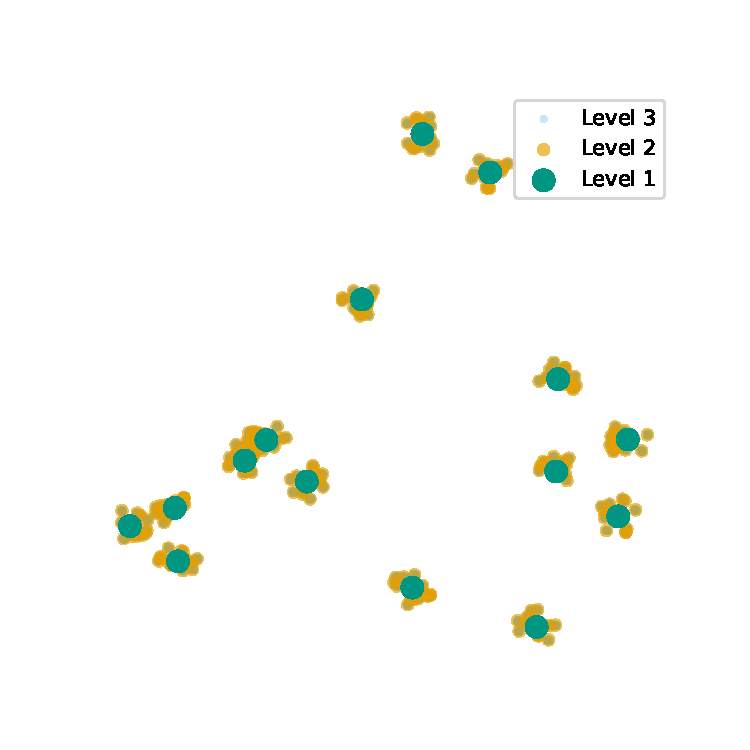
\includegraphics[width=\linewidth]{graphics/small.pdf}
		\caption{Too rapid radii decay.}
		\label{fig:radius_small}
	\end{subfigure}
	\hfill
	\begin{subfigure}{0.3\linewidth}
		\centering
		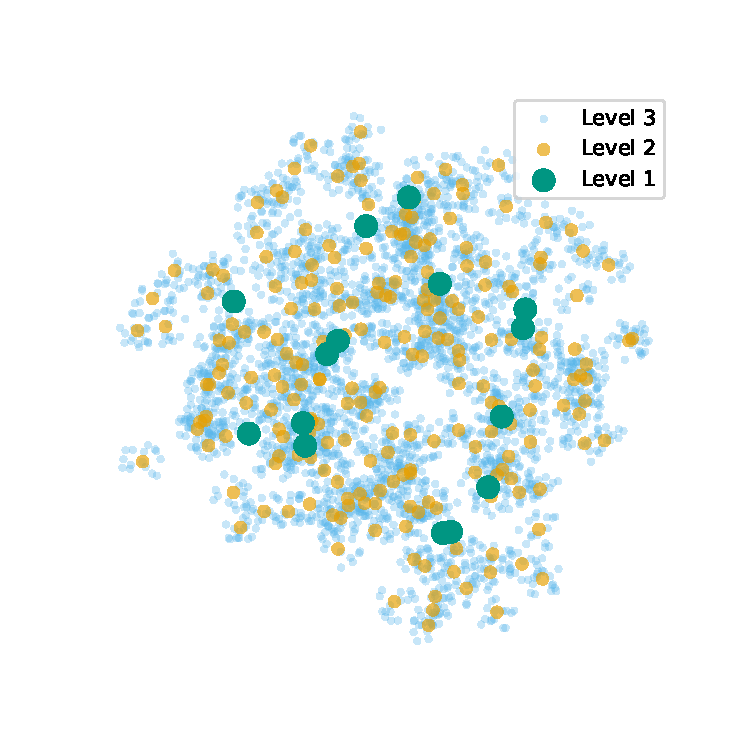
\includegraphics[width=\linewidth]{graphics/good.pdf}
		\caption{Well-tuned radii decay.}
		\label{fig:radius_good}
	\end{subfigure}
	\hfill
	\begin{subfigure}{0.3\linewidth}
		\centering
		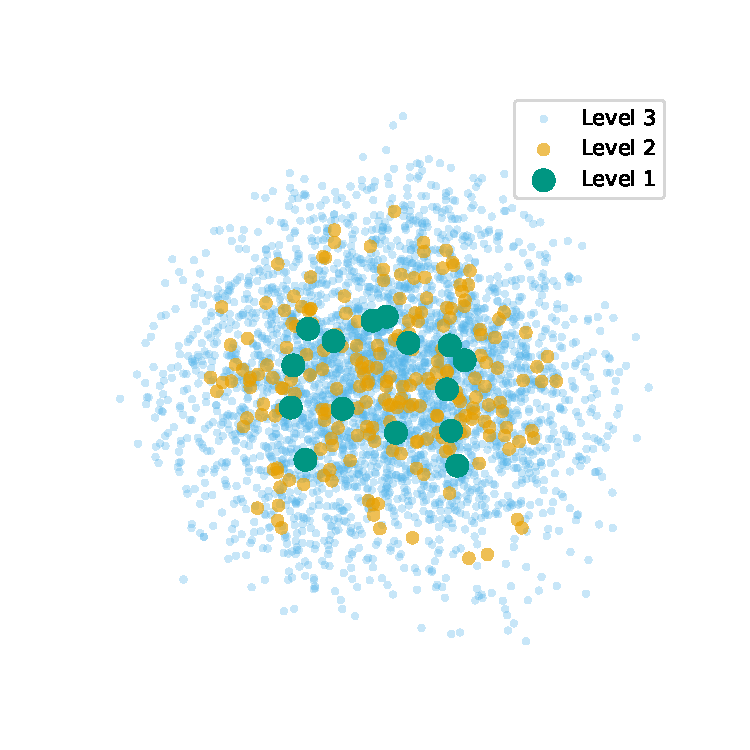
\includegraphics[width=\linewidth]{graphics/const.pdf}
		\caption{Constant radii.}
		\label{fig:radius_const}
	\end{subfigure}
	\caption{Illustration of the impact of different radii decay strategies on separator scaling. All other parameters held constant.}
	\label{fig:radius_compare}
\end{figure}

The degree of spatial overlap between regions expanded from different sites is fundamental to achieving desirable separator characteristics, as it dictates the strength of connectivity between hierarchical components.
The parameters \(f_i\), \(k_i\), and \(r_i\) jointly determine this overlap:
A higher expansion fraction \(f_i\) results in a greater number of nodes from the parent level being selected as expansion sites.
This reduces the average distance between chosen sites, causing their respective areas of influence for the current level to naturally adjoin or overlap significantly.
Increasing \(k_i\), the number of points generated per expansion site, primarily makes each local cluster denser.
Such high local density implies that partitioning these individual dense regions themselves requires larger separators, reflecting their increased internal complexity.
Simultaneously, by populating the same expansion radius \(r_i\) with more points, the average distances between points decrease on this level, increasing the likelihood of inter-cluster connections.
Compared to the influence of \(f_i\) and \(r_i\), the effect of \(k_i\) is minor.
The effect of the expansion radius \(r_i\) is direct: a larger radius straightforwardly increases the spatial extent of each new cluster, leading to more substantial overlap with adjacent expansion zones and, consequently, also contributing to larger overall separators due to increased linkage.
Radii at deeper hierarchical levels must also be scaled appropriately relative to those at higher levels to ensure desired structural properties and avoid unintended consequences on separator sizes.
Therefore, a careful balance of these parameters, \(f_i\), \(k_i\), and \(r_i\), is essential to cultivate a graph structure with the intended connectivity and separator properties.
The parameterization offers flexibility.
For instance, to simulate prominent \enquote{urban centers} at higher levels, a larger initial radius \(r_1\) might be employed.
This would typically be balanced by adjusting subsequent parameters, such as reducing \(f_2\) (selecting fewer centers from the points generated by these large initial expansions), to maintain overall structural integrity and desired separator characteristics.
However, such compensations have practical limits, if radii do not shrink sufficiently across levels, adjustments to \(f_i\) or \(k_i\) may not fully mitigate adverse effects on separator scaling.
For generating structures visually akin to road networks, allowing the number of active expansion sites to decrease at deeper hierarchical levels often yields favorable results.
This complements the inherent tendency of the generation process where all existing points are candidates for seeding new expansions, helping to manage density while still fostering hierarchical differentiation.
Plausible structures can emerge even with constant \(k_i\) values across levels, provided \(f_i\) and \(r_i\) are appropriately tuned.
For instance, the parameter set comprising level expansion fractions \(f_i = (1.0, 0.3, 0.2, 0.1)\), points per expansion site \(k_i = (50, 50, 50, 50)\), and expansion radii \(r_i = (1000, 424, 120, 17)\) produces graphs whose separator characteristics are illustrated in \Cref{fig:hier_delaunay_example_params_sep}.

\begin{figure}[tbhp]
	\centering
	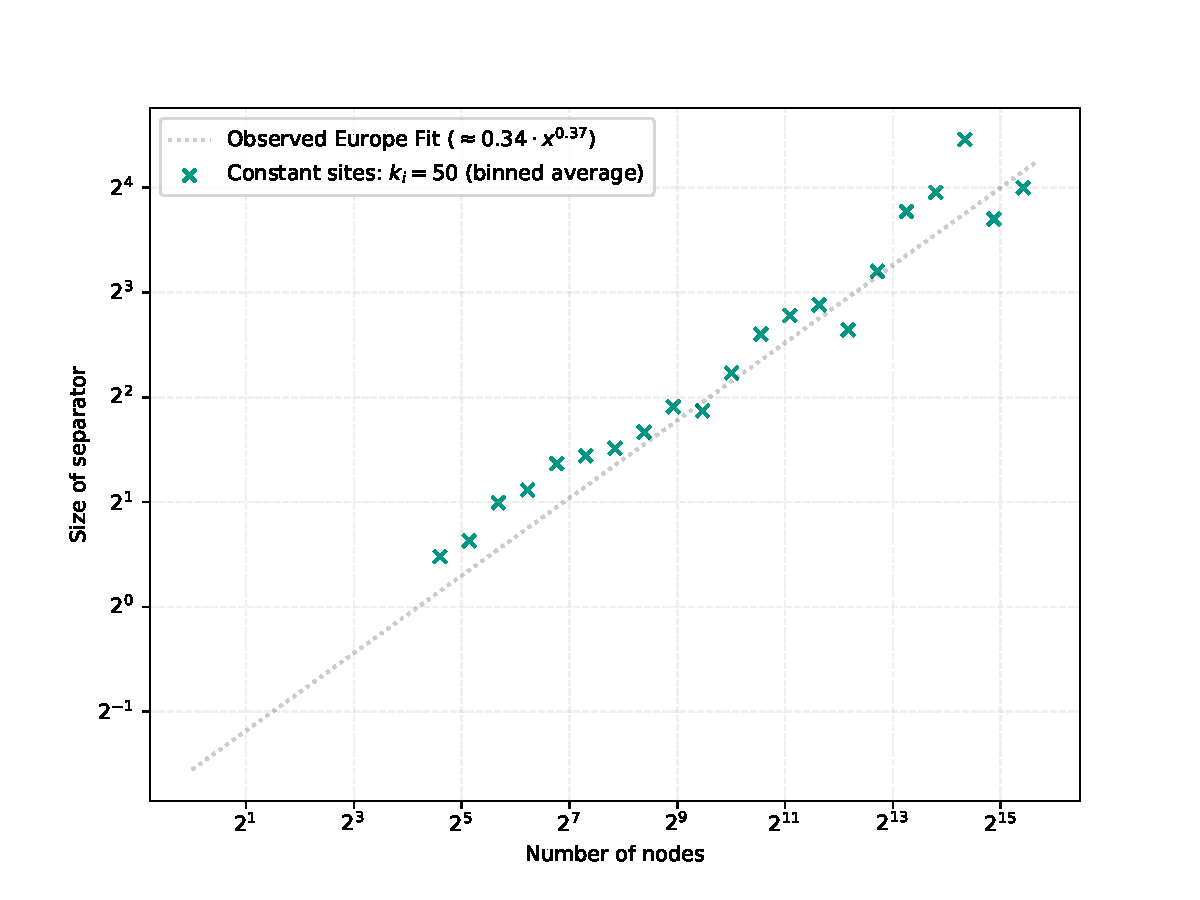
\includegraphics[width=0.7\linewidth]{graphics/hierachcial_delaunay_const_sites.pdf}
	\caption{Separator size scaling for a hierarchical Delaunay graph generated with constant expansion sites: \(f_i=(1.0, 0.3, 0.2, 0.1)\); \(k_i=(50, 50, 50, 50)\); \(r_i=(1000, 424, 120, 17)\). Separators were computed using InertialFlowCutter (tests with FlowCutter and KaHIP yielded similar asymptotic scaling).}
	\label{fig:hier_delaunay_example_params_sep}
\end{figure}

To further illustrate the interplay of these parameters, \Cref{fig:hier_delaunay_param_interplay} presents separator scaling plots for four different parameter configurations.
The baseline configuration, shown in \cref{fig:param_interplay_baseline}, is chosen to produce separators with characteristics similar to those observed in real road networks.
\Cref{fig:param_interplay_low_f2} then demonstrates the impact of significantly decreasing the expansion fraction for the second level (\(f_2\)) while other parameters are held constant relative to the baseline,
this results in a notable drop in separator sizes, indicative of a less interconnected structure.
Subsequently, \cref{fig:param_interplay_fix1_radii} shows that this reduction in separator size due to a low \(f_2\) can be counteracted by proportionally increasing the expansion radius of the second level (\(r_2\)) and the subsequent radii (\(r_3, r_4\)).
Alternatively, \cref{fig:param_interplay_fix2_k1} illustrates that increasing the number of points generated at the first level (\(k_1\)) can also compensate for the reduced \(f_2\), again achieving separator scaling similar to the baseline by enhancing overall density and connectivity from the initial expansion phase.

\begin{figure}[tbhp]
	\centering
	\begin{subfigure}{0.45\linewidth}
		\centering
		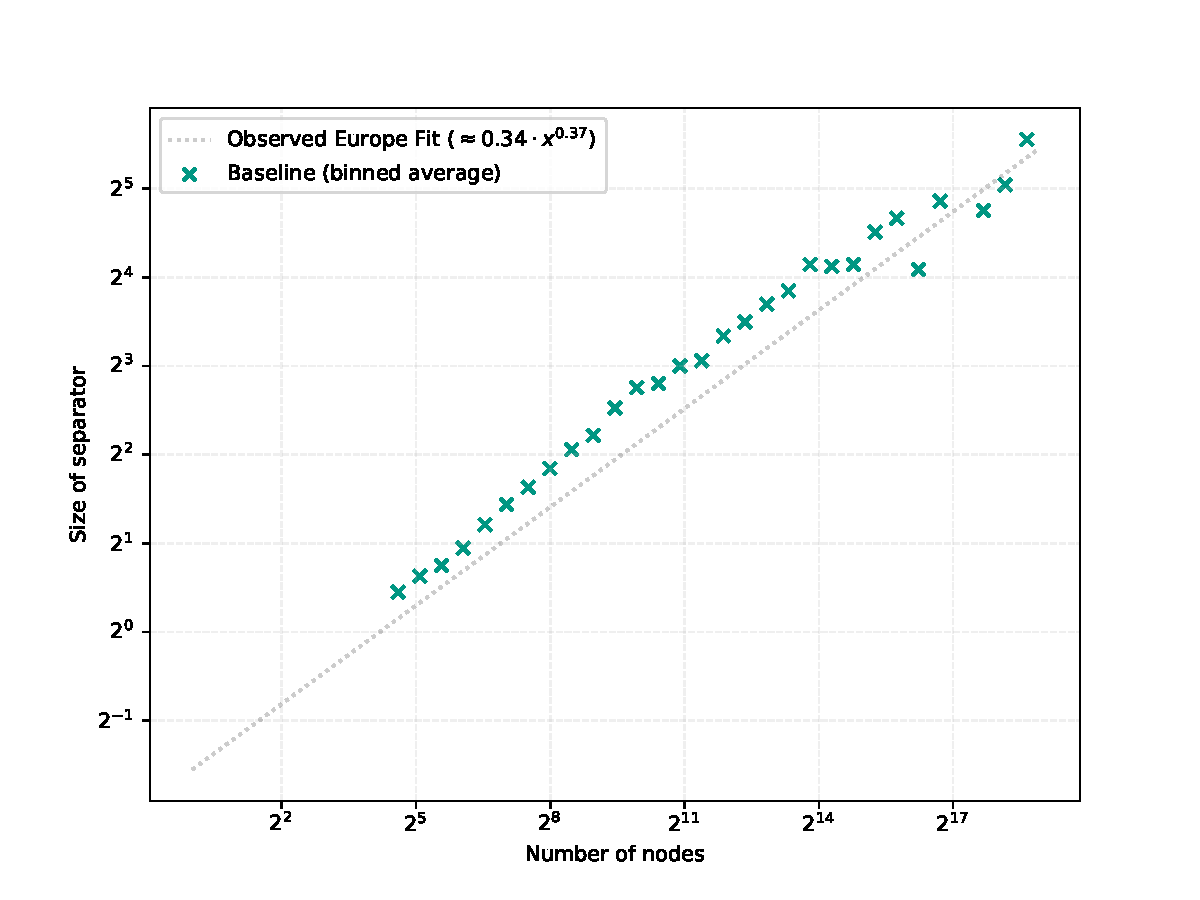
\includegraphics[width=\linewidth]{graphics/interplay_baseline.pdf}
		\caption{Baseline: \(f_i=(1.0, 0.5, 0.4, 0.3)\); \newline\(k_i=(200, 50, 35, 25)\); \(r_i=(1000, 141, 26, 6)\).}
		\label{fig:param_interplay_baseline}
	\end{subfigure}
	\hfill
	\begin{subfigure}{0.45\linewidth}
		\centering
		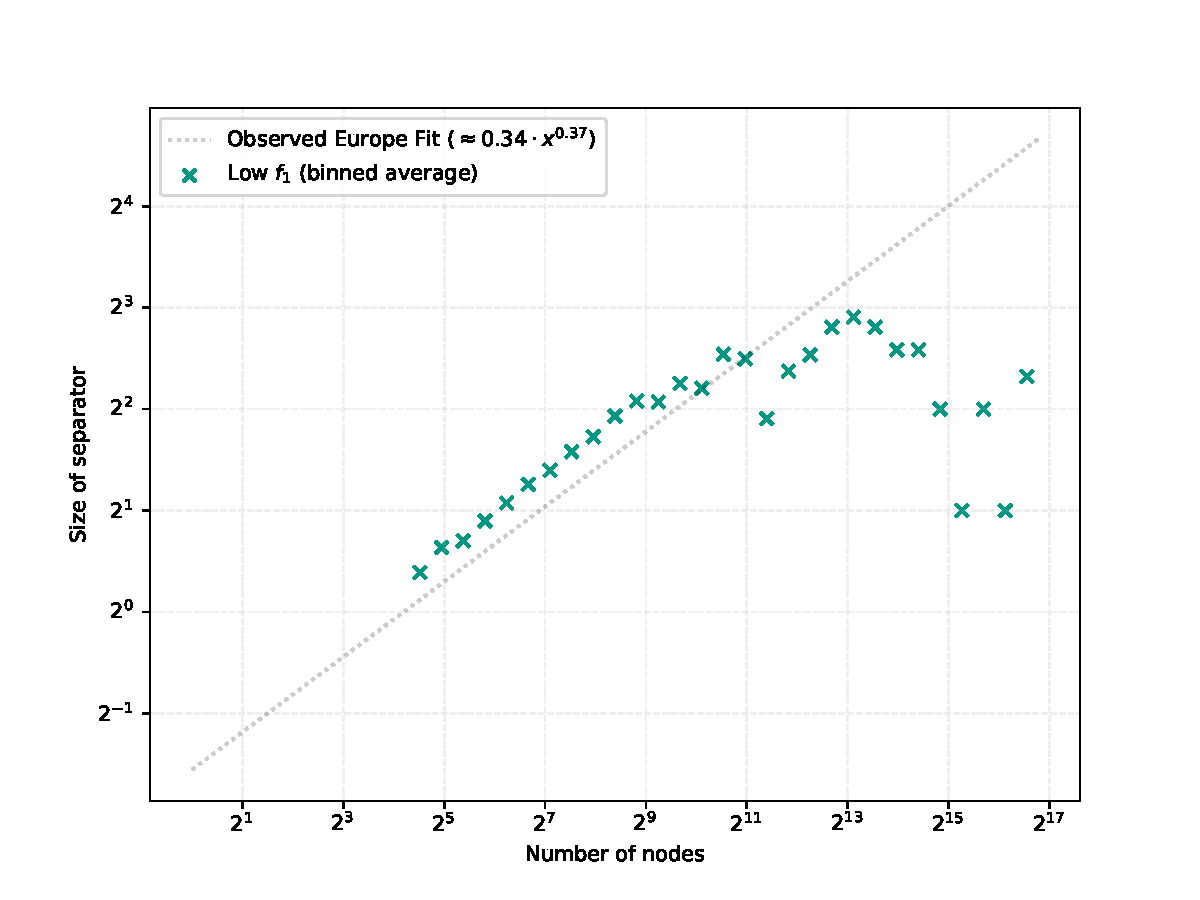
\includegraphics[width=\linewidth]{graphics/interplay_low_f1.pdf} % Filename implies f1, caption says f2
		\caption{Low \(f_2\): \(f_i=(1.0, \textcolor{red}{0.1}, 0.4, 0.3)\); \newline\(k_i=(200, 50, 35, 25)\); \(r_i=(1000, 141, 26, 6)\).}
		\label{fig:param_interplay_low_f2}
	\end{subfigure}

	\vspace{0.5cm}

	\begin{subfigure}{0.45\linewidth}
		\centering
		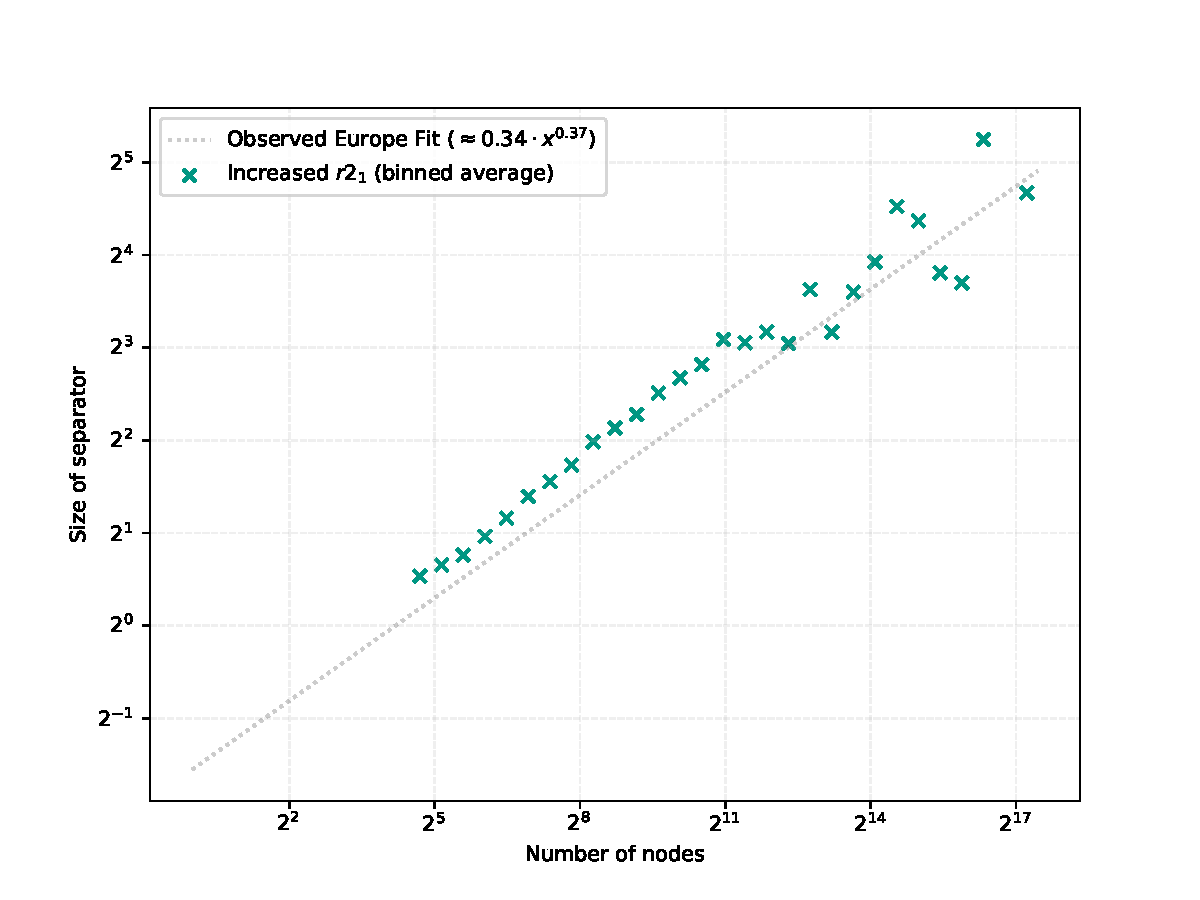
\includegraphics[width=\linewidth]{graphics/interplay_increased_r2.pdf}
		\caption{Fix 1 (Increase radii for low \(f_2\)): \newline\(f_i=(1.0, \textcolor{red}{0.1}, 0.4, 0.3)\); \(k_i=(200, 50, 35, 25)\); \(r_i=(1000, \textcolor{green}{283}, \textcolor{green!50}{52}, \textcolor{green!50}{11})\).}
		\label{fig:param_interplay_fix1_radii}
	\end{subfigure}
	\hfill
	\begin{subfigure}{0.45\linewidth}
		\centering
		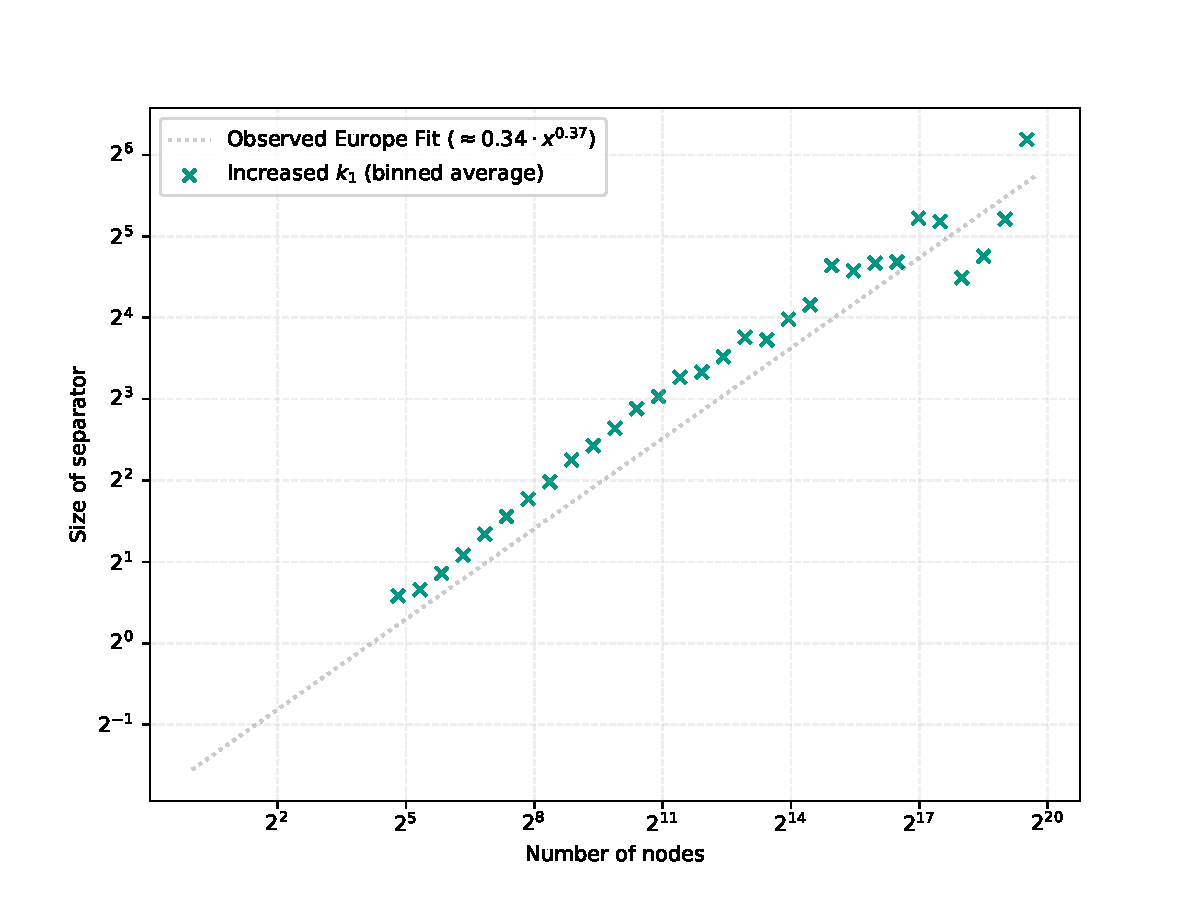
\includegraphics[width=\linewidth]{graphics/interplay_increased_k1.pdf}
		\caption{Fix 2 (Increase \(k_1\) for low \(f_2\)): \newline\(f_i=(1.0, \textcolor{red}{0.1}, 0.4, 0.3)\); \(k_i=(\textcolor{green}{1000}, 50, 35, 25)\); \(r_i=(1000, 141, 26, 6)\).}
		\label{fig:param_interplay_fix2_k1}
	\end{subfigure}
	\caption{Illustration of parameter interplay on separator size scaling in hierarchical Delaunay graphs. Graphs (b),(c) and (d) have a decreased \(f_2\) compared to the baseline (a). Paramter changes to fix the scaling are highlighted green. Separators were computed using InertialFlowCutter (tests with FlowCutter and KaHIP yielded similar asymptotic scaling).}
	\label{fig:hier_delaunay_param_interplay}
\end{figure}




















\subsection{Physical Barriers}
\label{sec:synthetic:physical_barriers}

To investigate the influence of physical features of varying scales on road network structure and separator sizes, ranging from large-scale elements like mountains or lakes to smaller features like challenging terrain or rivers, we explore a generative approach based on iterating Perlin noise functions across multiple scales.
The core idea is to use procedurally generated noise to define regions that are less favorable for node placement, simulating natural or man-made obstacles.
The foundational component of these approaches is Perlin noise, a type of gradient noise widely used for procedural texture generation \cite{perlin_image_1985}.
Unlike value noise, which interpolates random values assigned to a grid, Perlin noise generates a pseudo-random, continuous field by interpolating between random gradients assigned to grid points.
For any given point in space, its noise value is determined by its position relative to the surrounding grid points and the dot product with their corresponding gradient vectors.
A key characteristic of Perlin noise is that it produces a smooth, natural-looking texture with its energy concentrated around a specific frequency.
To create more complex patterns with details at multiple scales, several layers of Perlin noise with different frequencies and amplitudes are typically combined.
Our initial attempt utilizes a common method for generating additive fractal noise (often termed pink noise).
This process involves summing multiple layers of Perlin noise, where at each step, the sampling frequency doubles and the amplitude halves.
Sampling at a given point \((x,y)\) at scale \(s\) can also be thought of as sampling a universal noise at \((x \cdot s, y \cdot s)\).
Multiplying the point coordinates by the scale larger than 1 effectively compresses the noise pattern, increasing the frequency of the noise.
To avoid artifacts from sampling identical coordinates across different scales, we apply both scaling and translational offsets to the input coordinates for each noise layer: for instance, for a point \((x,y)\) and a given scale, the noise is sampled at \(((x + 3) \cdot \text{scale}, (y+3) \cdot \text{scale} )\).
If the scale values are chosen as powers of two, adding \(3 \cdot \text{scale}\) to a point, ensures that the noise samples at different scales do not overlap.
Points are then sampled in a domain, and their acceptance probability is modulated by the resulting smooth, cloud-like noise value at their location.
However, this additive approach produces noise that is too smooth, and the resulting \enquote{obstacles} are not sufficiently \enquote{hard} or prohibitive.
Graphs generated by accepting points based on this smooth additive fractal noise exhibit separator sizes scaling as \bigO{n^{1/2}}.
Alternative procedural noise types, such as Simplex noise or Brownian noise, likewise fail to produce the desired combination of relatively sharp boundaries and distinct features across multiple scales.
To create more defined, \enquote{harder} obstacle boundaries across multiple scales, we develop an alternative approach using multiplicative Perlin noise.
For each point \(p\), Perlin noise is first sampled at \(L\) different scales (often referred to as octaves), where the frequency typically doubles at each successive scale.
The output from the Perlin noise function for each of these \(L\) scales, usually in the range \([-1, 1]\), is then normalized to \([0, 1]\).
Finally, the overall noise value for the point is determined by the product of these \(L\) normalized values.
As the number of noise scales increases, the resulting product tends towards zero.
To transform this continuous output into a binary map of allowed versus disallowed regions, we apply a noise threshold (e.g., \(0.5^L\)).
A point is considered in an \enquote{allowed} region if its final product value is greater than the noise threshold,
otherwise, it is \enquote{disallowed}.
This method yields a binary noise field with sharp boundaries and features at various frequencies, as \cref{fig:multiplicative_binary_noise_viz} illustrates.
One could also consider normalizing the product of the noise values by taking the \(L\)-th root of the product and using this value as a probability if a point is in an allowed region or not.
This however yields quadratic scaling behavior for the separator size, as the resulting noise field is too smooth and does not produce sufficiently distinct obstacle regions.

\begin{figure}[tbhp]
	\centering
	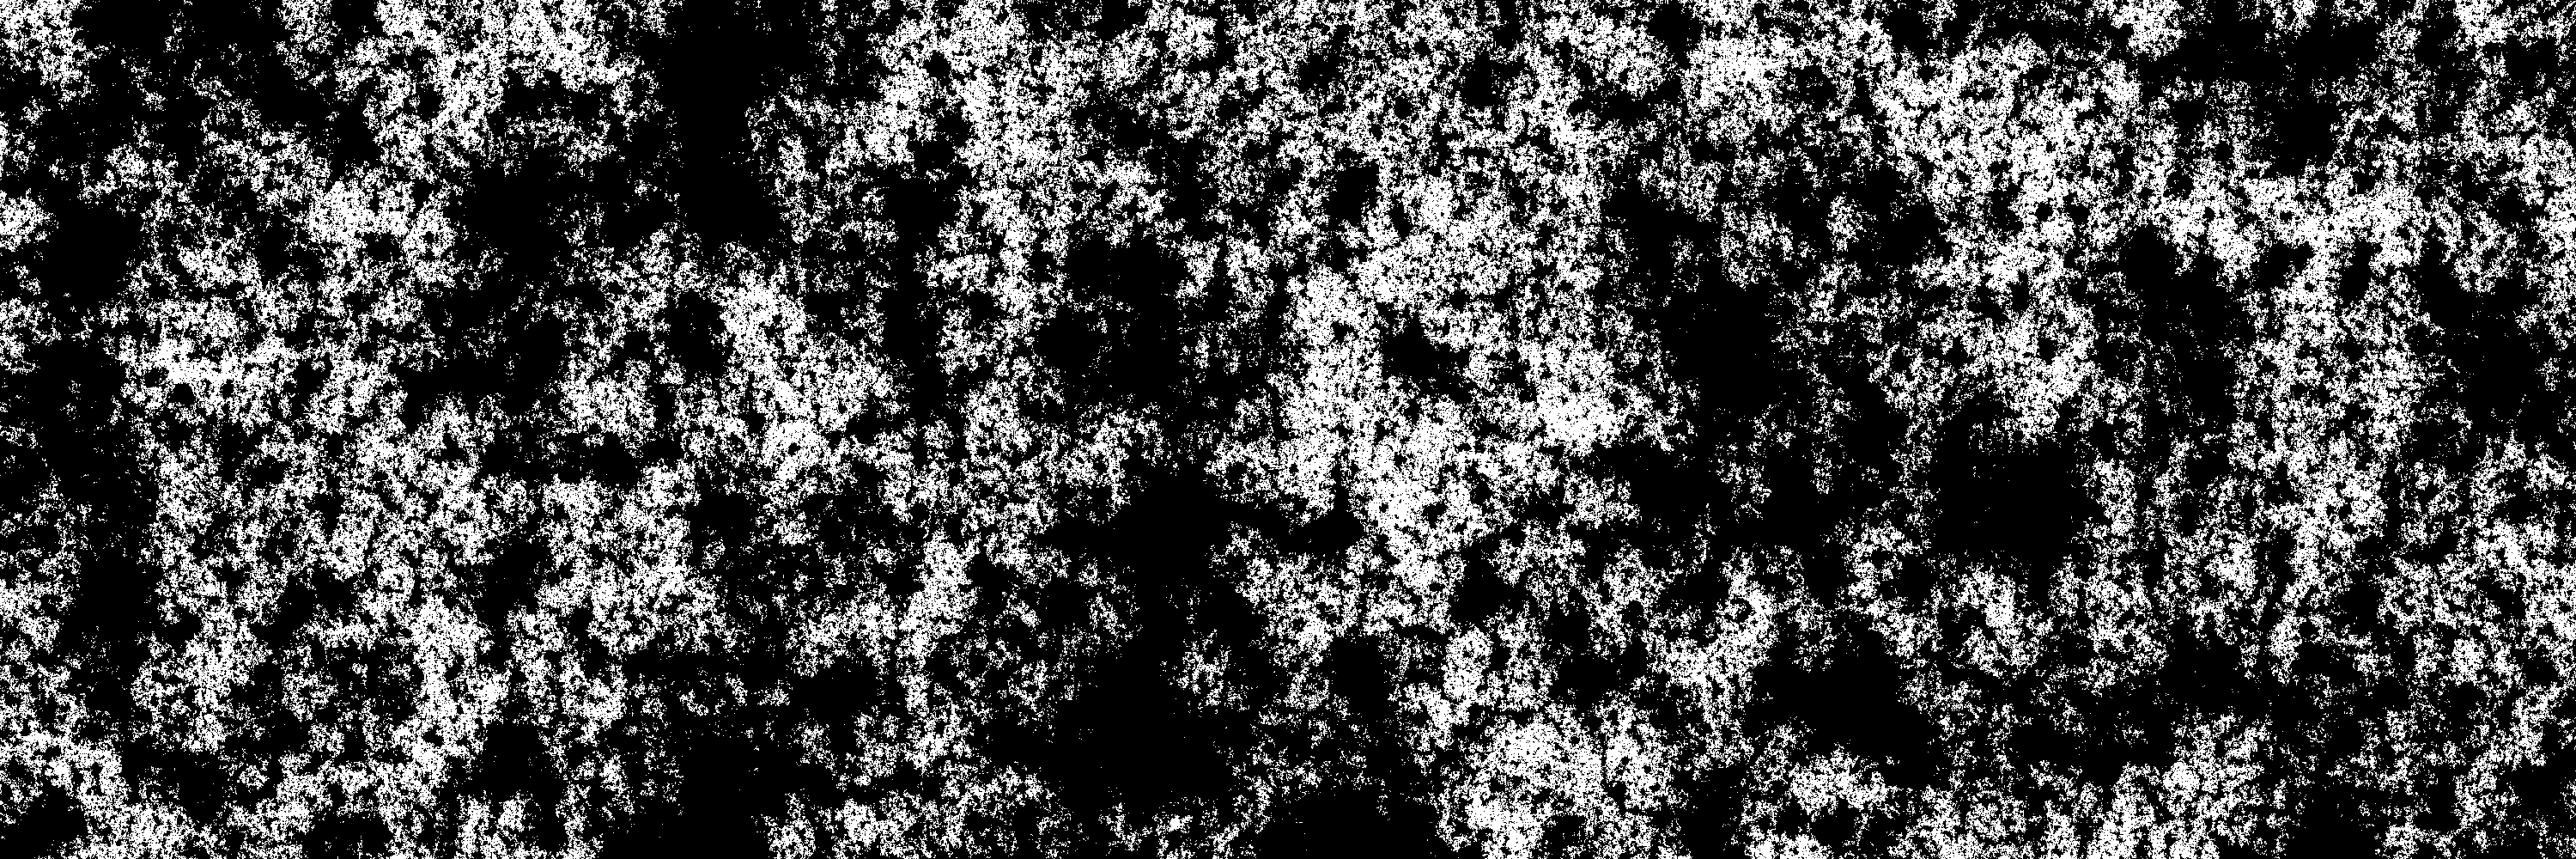
\includegraphics[width=\linewidth]{graphics/noise_image.png}
	\caption{Visualization of the multiplicative binary Perlin noise used to define obstacle regions across multiple scales.}
	\label{fig:multiplicative_binary_noise_viz}
\end{figure}

The graph generation algorithm then utilizes this multiplicative binary Perlin noise to place vertices, as detailed in \cref{alg:fractal_noise_point_sampling}.
Candidate points are randomly sampled within a predefined domain (e.g., a unit circle).
The noise value, as described above, is computed at each candidate point's location.
If this value indicates an \enquote{allowed} region, the point is accepted and added to the graph's vertex set,
otherwise, it is rejected, and a new candidate is sampled.
This process continues until the desired number of \(n\) vertices is collected.
Achieving the desired separator scaling for a larger number of vertices appears to necessitate an increased number of noise scales.
No clear upper bound on the number of applicable scales is apparent.
Increasing the number of scales introduces a slight computational overhead.
However, this does not substantially affect the overall performance of the graph generation process.
Our implementation successfully generates graphs with vertex counts \(n \in \{10^4, 10^5, 10^6, 10^7\}\) using \(L=11\) scales.
The generation method demonstrates scalability, producing graphs with up to 300 million nodes.
For larger graphs, we primarily rely on using the Relative Neighborhood Graph (RNG) creation instead of a Delaunay triangulation with the following edge pruning because the RNG is more efficient to compute for larger point sets.
Further experiments are constrained by limitations in underlying libraries, which employ 32-bit integers for internal processing.
Once the \(n\) points are generated, a global Delaunay triangulation is performed on this point set.
Subsequently, the same edge pruning step detailed in the Hierarchical Delaunay Generation section (see \cref{alg:prune_edges}) is applied to achieve a target average degree and refine the graph structure.
An example of a graph generated using this method and its observed separator scaling are shown in \cref{fig:fractal_noise_graph_results}.

\begin{algorithm}[tbhp]
	\Input{Target number of points \(n\), \\
		\(L\) noise scales \(s_i\)}
	\Output{Geometric graph \(G\)}
	\BlankLine
	\(P \longleftarrow \emptyset\)\;
	\While{\(|P| < n\)}{
		\(p \longleftarrow\) randomPointInUnitCircle()\;
		\BlankLine
		noise \(\longleftarrow \prod_{i=1}^{L} \text{perlinNoise}(p \cdot s_i)\)\;
		\BlankLine
		\If{\(\text{noise} > 0.5^{L}\)}{
			\(P \longleftarrow P \cup \{p\}\)\;
		}
	}
	\(G \longleftarrow\) delaunay(\(P\))\;
	pruneEdges(\(G\))\;
	\Return{\(G\)}\;
	\caption{Graph generator using Multiplicative Binary Perlin Noise}
	\label{alg:fractal_noise_point_sampling}
\end{algorithm}

\begin{figure}[tbhp]
	\centering
	\begin{subfigure}{0.35\linewidth}
		\centering
		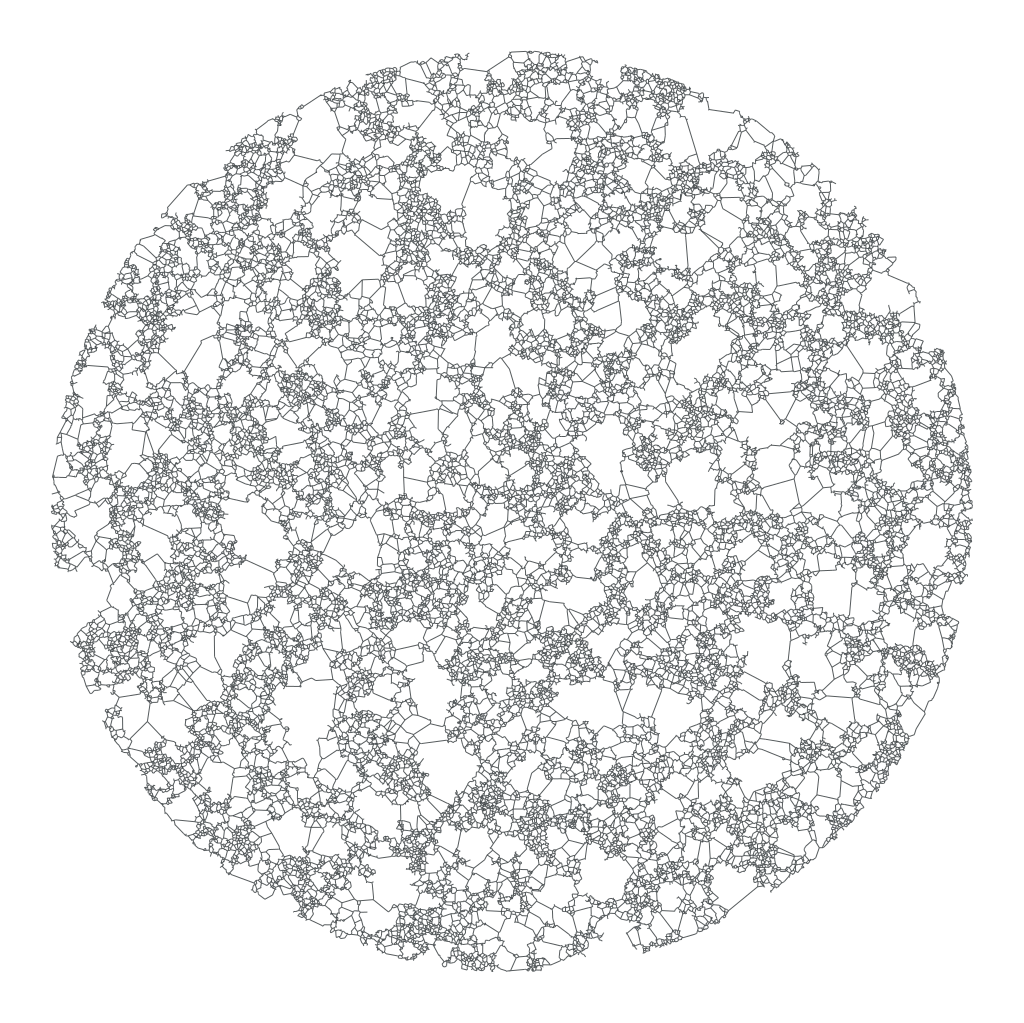
\includegraphics[width=\linewidth]{graphics/noise.png}
		\caption{Graph generated using multi-scale Perlin noise-based point sampling (\(n = 10^5\)).}
		\label{fig:fractal_noise_graph_viz}
	\end{subfigure}
	\hfill
	\begin{subfigure}{0.55\linewidth}
		\centering
		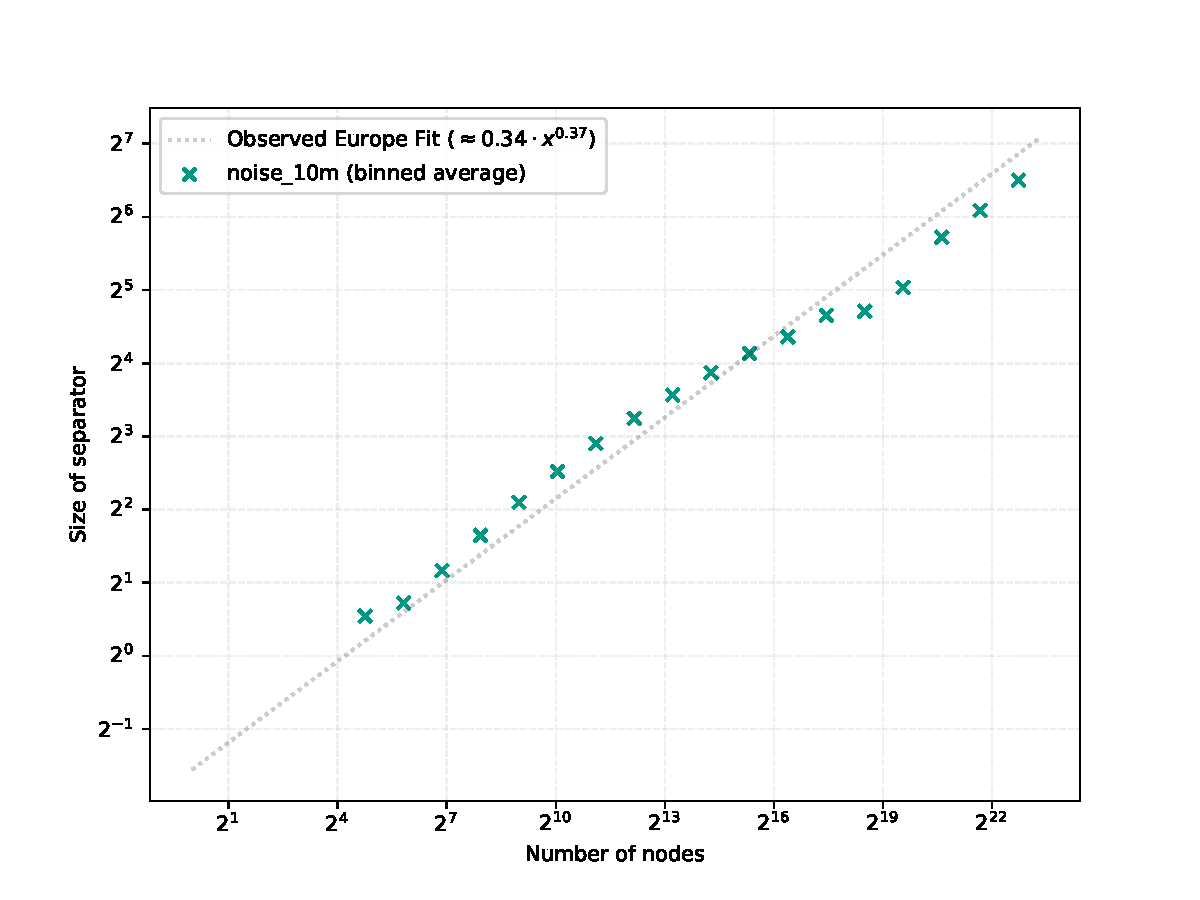
\includegraphics[width=\linewidth]{graphics/noise_10m.pdf}
		\caption{Separator scaling for the multi-scale Perlin noise graph.}
		\label{fig:fractal_noise_graph_sep_plot}
	\end{subfigure}
	\caption{Synthetic graph generated using multiplicative binary Perlin noise and its separator scaling. Separators were computed using InertialFlowCutter (tests with FlowCutter and KaHIP yielded similar asymptotic scaling).}
	\label{fig:fractal_noise_graph_results}
\end{figure}

This generation process does not directly prevent Delaunay edges from spanning the \enquote{obstacle} regions (areas with low composite noise values where no points are placed).
However, it ensures that no vertices, and thus no potential navigation hubs or major junctions, are located within these simulated forbidden zones.
Furthermore, the subsequent edge pruning step tends to remove many of the long, redundant edges that might span these empty regions, preserving only those deemed more critical for connectivity, akin to bridges over rivers or passes through mountainous terrain.
The primary success of the multi-scale Perlin noise model lies in its ability to naturally generate graphs with the desired separator properties.
Requiring only the selection of a suitable range of scales, rather than extensive fine-tuning, this method produces graphs whose separator sizes scale approximately as \bigO{n^{0.37}}.
This result is crucial, as the exponent aligns almost exactly with the scaling empirically observed in real-world road networks.

\paragraph{Ablation Studies on Noise Scales}

We also investigate whether the full spectrum of noise scales is necessary to achieve this result.
Experiments are conducted using only high-frequency scales and only low-frequency scales.
The resulting noise patterns and separator scaling comparisons are illustrated in \cref{fig:noise_layer_ablation}.
When using only high-frequency scales, the separators for smaller subgraphs (identified through nested dissection) align well with the desired trend.
However, as the graph size or region under consideration increases, the separator sizes revert to an \bigO{n^{1/2}} trend, because large-scale obstacle features (which would be defined by low frequencies) are absent.
Conversely, the model using only low-frequency scales exhibits a more complex, multi-stage scaling behavior.
For smaller subgraphs, which fit entirely within the open regions defined by the noise, separators tend to scale as \bigO{n^{1/2}}, similar to standard Delaunay triangulations in unobstructed space.
As subgraphs become large enough to span these regions, the low-frequency obstacles themselves begin to define the partitions, causing a \enquote{drop-off} from this initial trend to relatively smaller separator sizes.
However, for the final top-level separators, we observe a steep increase in size.
To investigate this further, we generated a much larger graph with \(\approx 250\) million nodes.
This larger experiment confirms the same overall pattern of a drop-off followed by an increase for the largest separators, but the transition points are shifted to larger subgraph sizes.
This indicates that the subgraph size at which the low-frequency obstacles become effective separators is relative to the total number of nodes in the graph being partitioned.

\begin{figure}[tbhp]
	\centering
	\begin{subfigure}{0.25\linewidth}
		\centering
		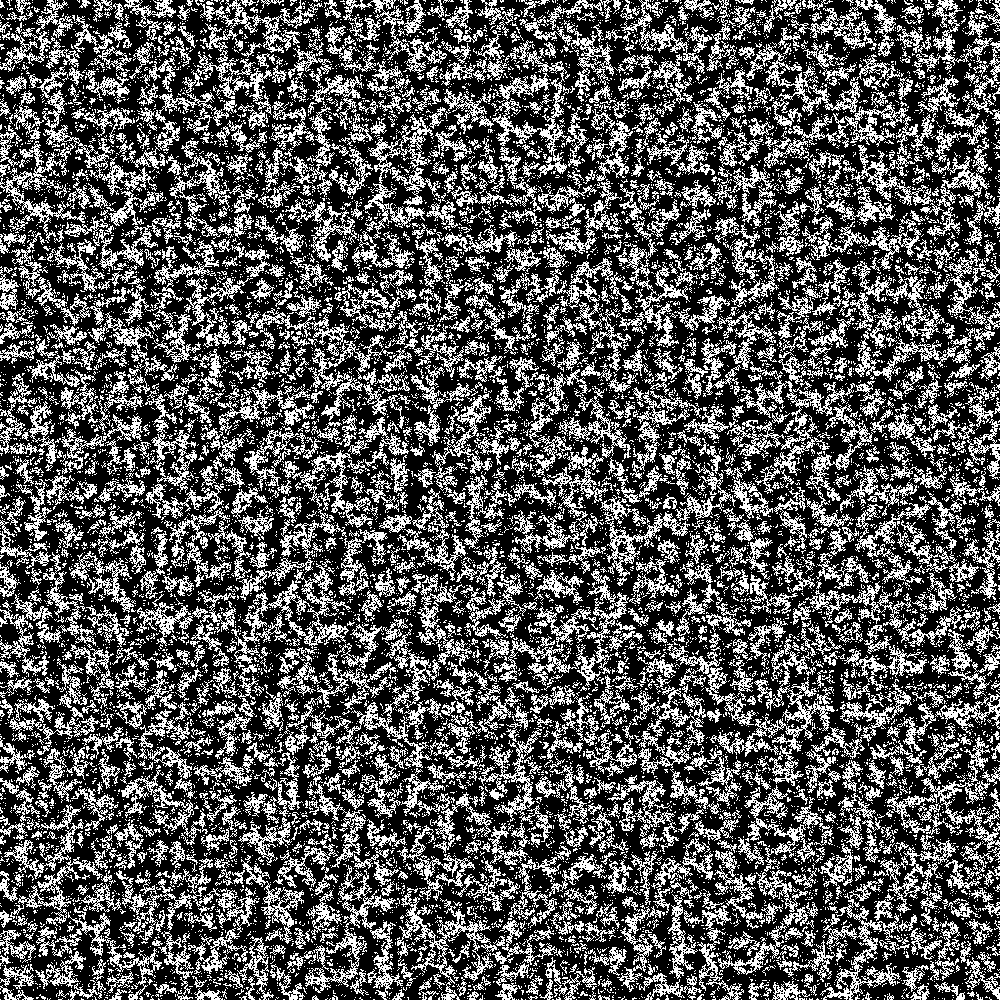
\includegraphics[width=\linewidth]{graphics/noise_high.png}
		\caption{Noise from high-frequency scales only.}
		\label{fig:noise_high_freq_viz}
	\end{subfigure}
	\hfill
	\begin{subfigure}{0.25\linewidth}
		\centering
		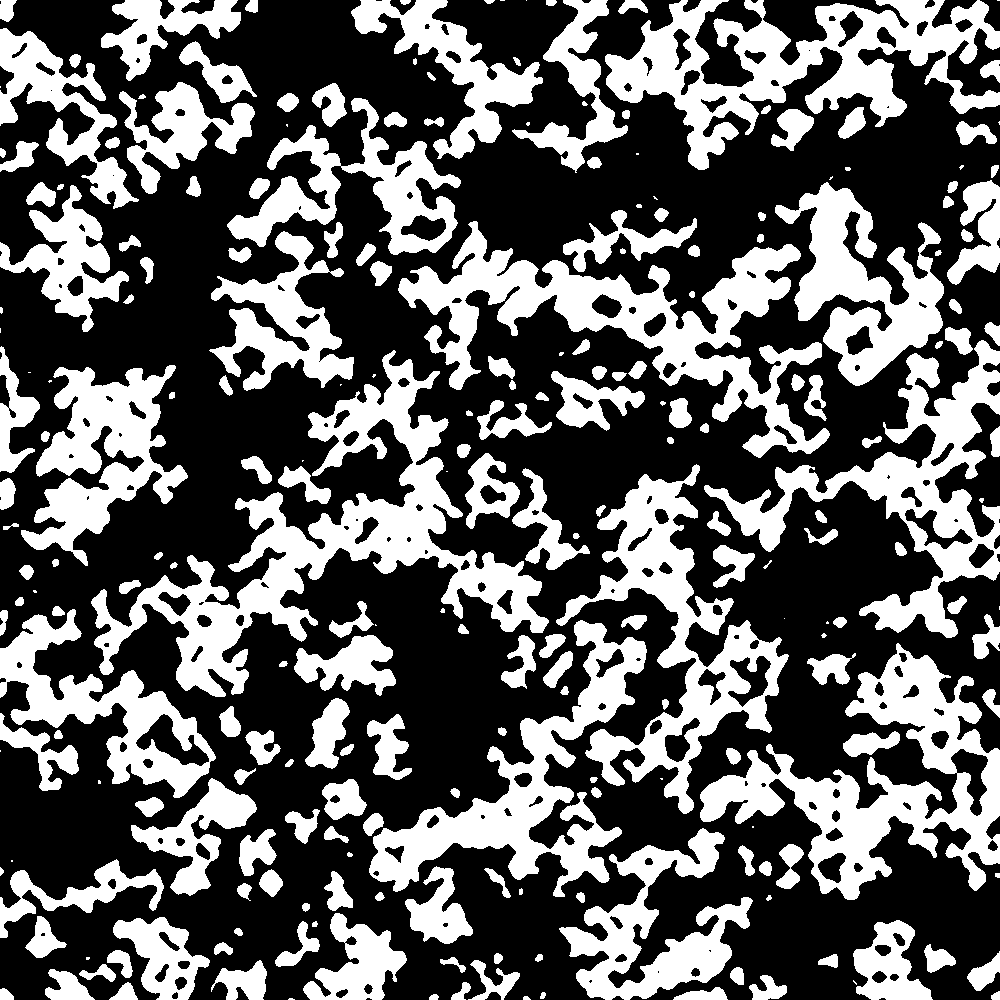
\includegraphics[width=\linewidth]{graphics/noise_low.png}
		\caption{Noise from low-frequency scales only.}
		\label{fig:noise_low_freq_viz}
	\end{subfigure}
	\hfill
	\begin{subfigure}{0.45\linewidth}
		\centering
		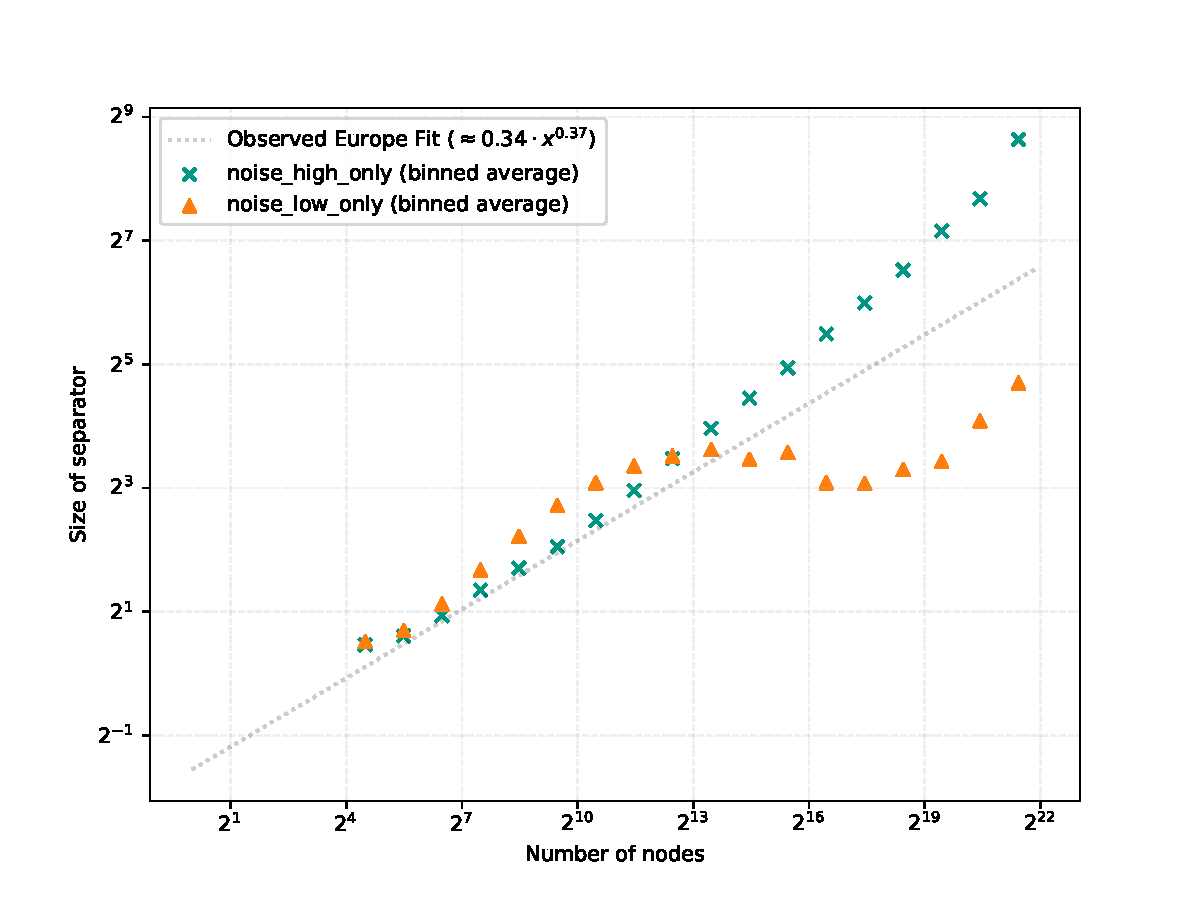
\includegraphics[width=\linewidth]{graphics/noise_high_vs_low_only.pdf}
		\caption{Separator scaling: high-freq. vs. low-freq. only.}
		\label{fig:noise_ablation_sep_plot}
	\end{subfigure}
	\caption{Impact of using only high-frequency versus only low-frequency Perlin noise scales on (a, b) noise patterns and (c) separator scaling. Separators were computed using InertialFlowCutter (tests with FlowCutter and KaHIP yielded similar asymptotic scaling).}
	\label{fig:noise_layer_ablation}
\end{figure}

These studies therefore show that using a combination of multiple noise scales, representing obstacles of various sizes, is key to consistently achieving small separator sizes across a wide range of graph dimensions with this multi-scale Perlin noise method.
This reliance on features defined across different scales to create a complex, layered obstacle landscape is conceptually similar to the explicit hierarchical graph generation methods explored earlier (e.g., \cref{sec:hierarchical_delaunay_generation}),
in both approaches, such multi-scale or hierarchical structuring is vital for achieving the desired separator properties, as is demonstrated in our noise model experiments where the favorable separator scaling breaks down if an insufficient range of scales is employed.

\paragraph{Alternative Graph Construction: k-Nearest Neighbors}

While the primary approach described above utilizes a Delaunay triangulation followed by pruning on the noise-sampled points, we also explored an alternative graph construction method using k-Nearest Neighbors (k-NN) on the same underlying point sets.
For these non-uniformly distributed points, a consequence of the noise-based acceptance criteria, a \(k=3\), which often suffices to ensure reasonable connectivity for uniformly sampled points, proved insufficient.
We found that a value of \(k=5\) was generally necessary to achieve a largely connected graph.
Interestingly, k-NN graphs constructed from these noise-sampled points exhibited separator sizes that were substantially smaller than our target \bigO{n^{0.37}}.
\Cref{fig:knn_vs_delaunay_noise_points} illustrates this comparison.
Visually comparing a k-NN graph (\cref{fig:knn_noise_graph_viz_comp}) with a graph derived from the Delaunay-based approach on the same noise-sampled point set (\cref{fig:delaunay_noise_graph_viz_comp}) reveals that the k-NN graph possesses significantly fewer long edges.
This characteristic arises because the k-NN construction inherently limits connections to only the \(k\) closest neighbors.
Consequently, edges are less likely to span large low-noise regions (our simulated obstacles), particularly if a point's \(k\) nearest neighbors all reside on the same side of such a zone.
Marginally increasing \(k\) does not fundamentally alter this effect, as it still restricts connections to a local neighborhood.
The limited long-range connectivity of the k-NN rule appears to cascade through recursive partitioning.
This leads to disproportionately small separators for larger graphs, while smaller, more internally-connected subgraphs can exhibit comparatively larger separators.
For substantially larger values of k, such as k=50, the separators exhibit quadratic scaling.

\begin{figure}[tbhp]
	\centering
	\begin{subfigure}{0.27\linewidth}
		\centering
		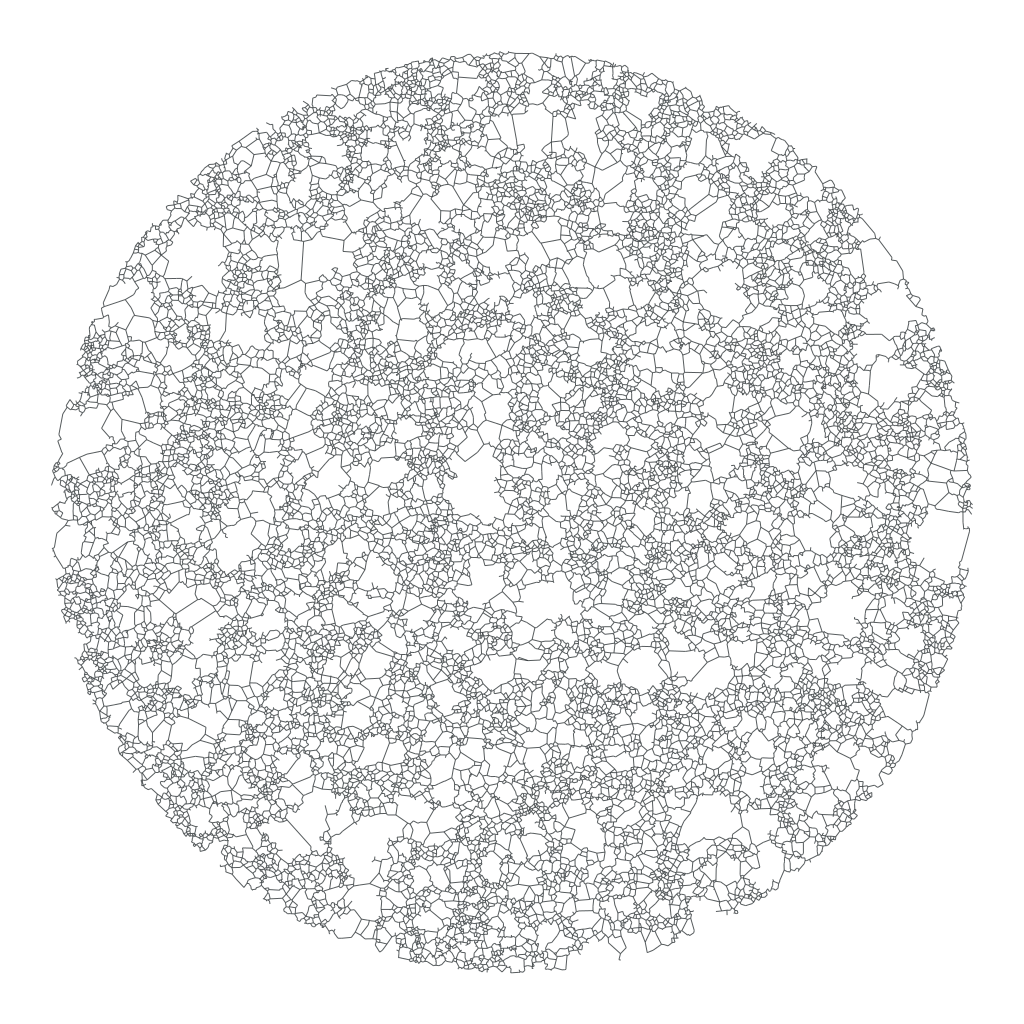
\includegraphics[width=\linewidth]{graphics/noise_rng_small.png}
		\caption{Delaunay subgraph on noise-sampled points. \\}
		\label{fig:delaunay_noise_graph_viz_comp}
	\end{subfigure}
	\hfill
	\begin{subfigure}{0.27\linewidth}
		\centering
		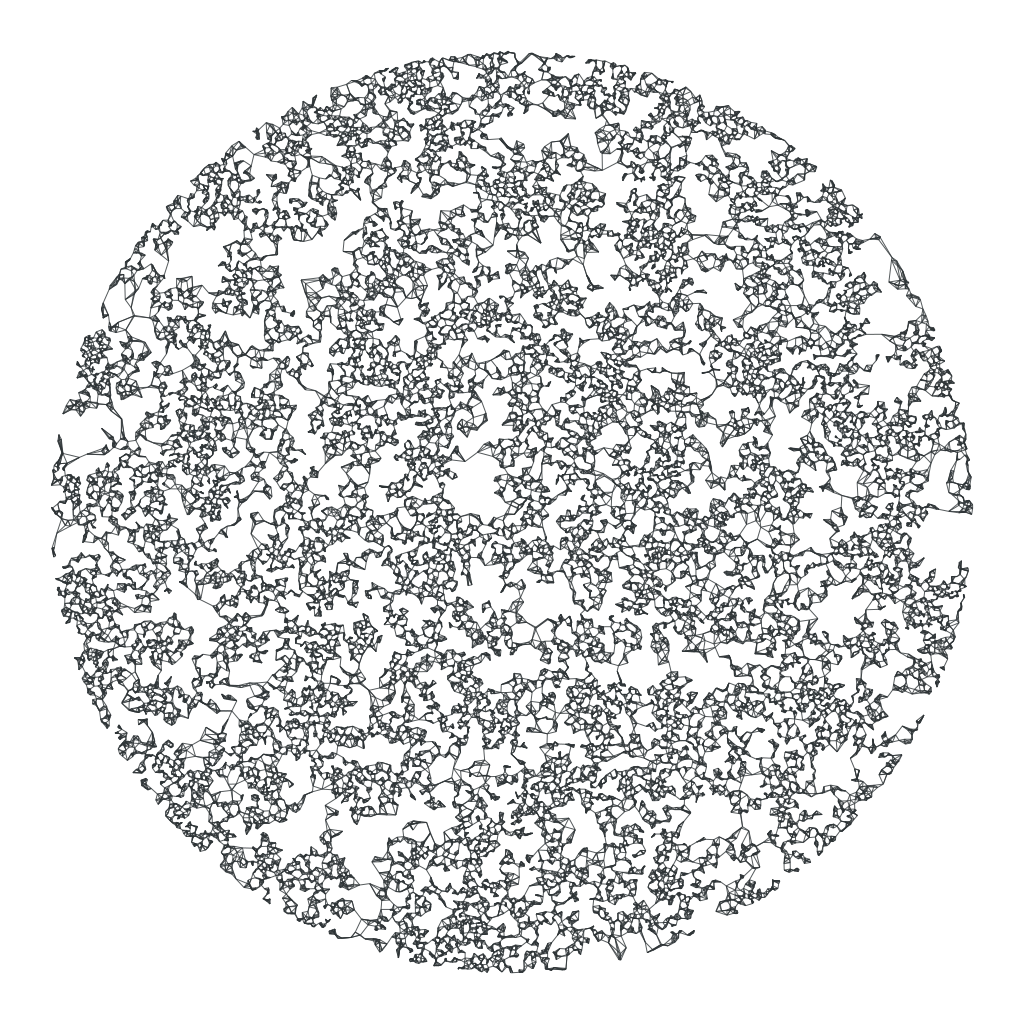
\includegraphics[width=\linewidth]{graphics/noise_knn_small.png}
		\caption{k-NN graph (\(k=5\)) on the same noise-sampled point set.}
		\label{fig:knn_noise_graph_viz_comp}
	\end{subfigure}
	\hfill
	\begin{subfigure}{0.4\linewidth}
		\centering
		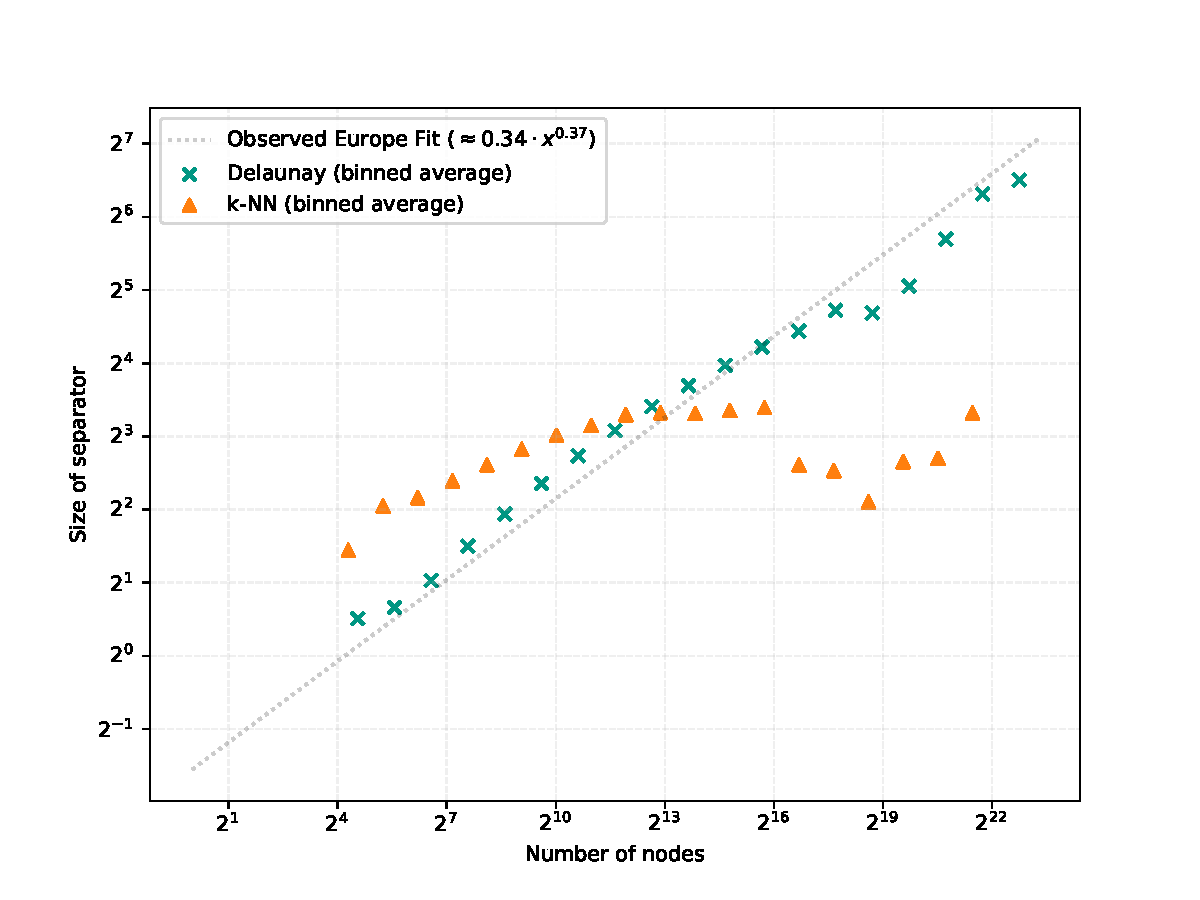
\includegraphics[width=\linewidth]{graphics/noise_knn_vs_rng.pdf}
		\caption{Separator scaling: Delaunay-based vs. k-NN based.}
		\label{fig:knn_delaunay_noise_sep_compare}
	\end{subfigure}
	\caption{Comparison of graph structures and separator scaling for Delaunay-derived graphs versus k-NN graphs on identical noise-sampled point sets. Separators were computed using InertialFlowCutter (tests with FlowCutter and KaHIP yielded similar asymptotic scaling).}
	\label{fig:knn_vs_delaunay_noise_points}
\end{figure}

This comparison highlights a distinction between the two graph construction methods.
A hierarchical point distribution, as generated by our multi-scale noise, appears to be a necessary but not sufficient condition for achieving the target separator scaling.
The resulting separator scaling also appears to depend on the specific connectivity pattern induced by the graph construction algorithm.
In contrast to the k-NN graph, the Delaunay triangulation permits the creation of long-range edges that span large, empty regions (our simulated obstacles).
These \enquote{bridge} edges appear to contribute to a more globally integrated graph structure, which may explain why this model avoids the higher degree of fragmentation and the smaller separator sizes observed with the more locally-restricted k-NN approach.

\paragraph{Comparison with Real-World Hop Distribution}

Given the success of the multi-scale Perlin noise model in replicating separator scaling, we further investigate its potential as a general-purpose synthetic road network generator by comparing its structural properties to the real Europe road network.
For this comparison, we focus on the hop distance distribution rather than the weighted distance distribution.
A direct comparison of geographic path lengths is not as insightful here, as this metric is heavily influenced by the overall shape of the embedding domain.
Our model samples points within a compact circle, which naturally produces a different distance profile than the complex and elongated geography of the European continent.
The hop distribution, in contrast, better reflects the intrinsic topological structure and hierarchical connectivity of a graph, making it a more suitable metric for evaluating the model's realism independent of its boundary shape.

To proceed with this comparison, we analyze three key graphs.
First, the real DIMACS Europe road network is pre-processed by contracting its degree-2 vertices, reducing it from approximately 18 million to 15 million nodes; this forms our empirical benchmark.
Second, to establish a baseline, we generate a full Delaunay triangulation on 15 million noise-sampled points, which by construction has no degree-2 nodes to contract.
Third, we generate a graph using our primary noise-based method: starting with 18 million points, performing a Delaunay triangulation, applying the pruning step from \cref{alg:prune_edges}, and finally contracting degree-2 nodes, which results in a graph of approximately 14 million nodes.

The resulting hop distributions are shown in \cref{fig:hop_dist_comparison_noise_vs_europe}.
Both synthetic graphs lack the extreme outliers (very long hop paths) of the real Europe graph, a discrepancy likely attributable to the differing domain shapes.
A key finding emerges from the comparison: the pruned synthetic graph is topologically much less efficient than the real network, with a significantly smaller fraction of nodes reachable in few hops.
Interestingly, the unpruned, full Delaunay triangulation provides a better approximation of the real network's hop distribution, exhibiting a similar peak, which is expected given its higher average degree naturally facilitates shorter hop paths.

This analysis leads to a crucial insight into our pruning strategy.
While the pruning method successfully achieves a realistic average degree and visual appearance, it appears to do so by removing too many of the structurally important long-range edges created by the Delaunay triangulation.
These edges are vital for a network's topological efficiency (i.e., short hop paths).
This suggests that while our noise-based point sampling creates a realistic foundation, a more sophisticated pruning strategy—one that better distinguishes between redundant local edges and essential long-range "highway" connections—is required to create a synthetic generator that accurately reproduces both separator scaling and hop distribution.

\begin{figure}[tbhp]
	\centering
	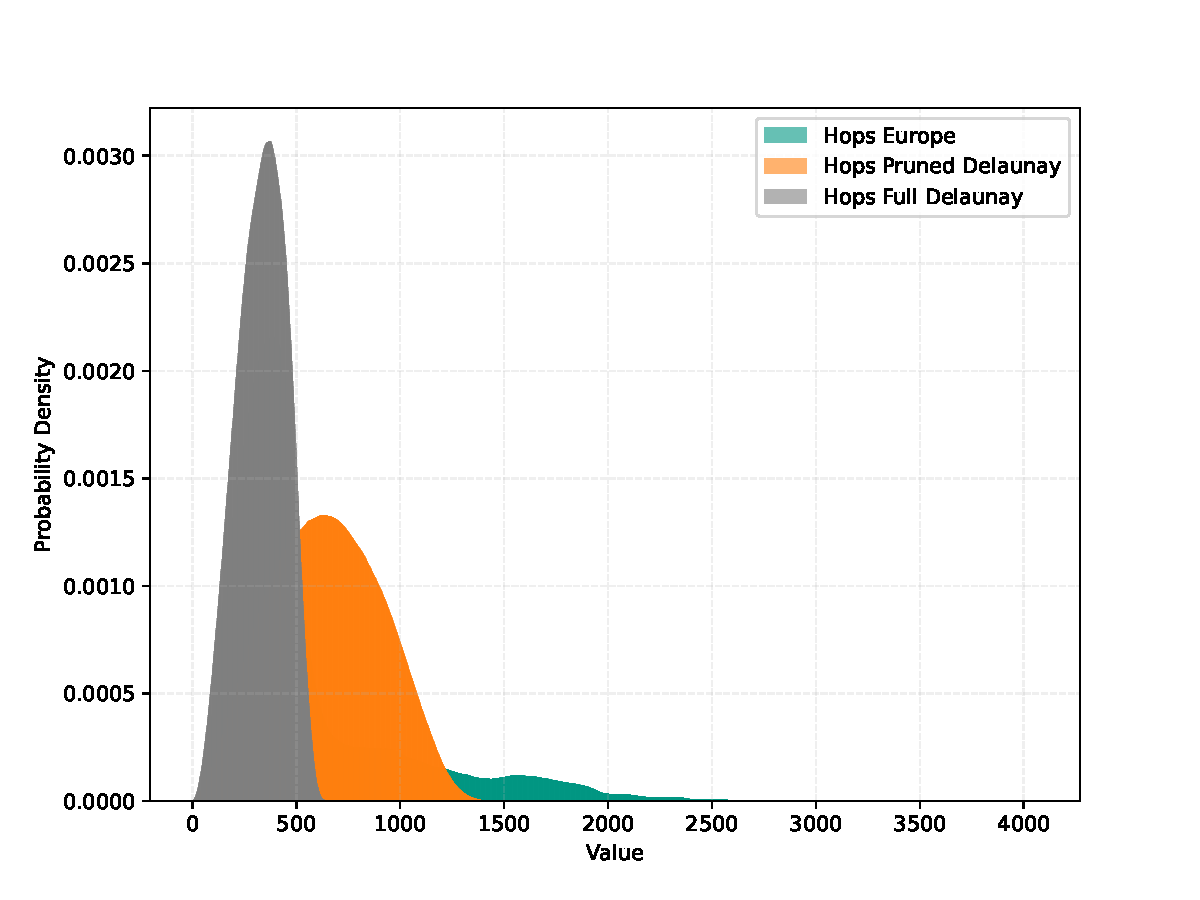
\includegraphics[width=0.7\linewidth]{graphics/hop_compare_noise_europe.pdf}
	\caption{Comparison of hop distance distributions of the Europe and multi-scale Perlin noise graphs. Graphs have their degree-2 nodes contracted.}
	\label{fig:hop_dist_comparison_noise_vs_europe}
\end{figure}
